\documentclass[a4paper,10pt,draft]{book}
\usepackage{graphicx} %\usepackage[utf8]{inputenc}
% center all figures:
\makeatletter
\g@addto@macro\@floatboxreset\centering
\makeatother

\usepackage{bbold}

\usepackage{makeidx}

\makeindex


\usepackage{amsmath}
\usepackage{bm}

\usepackage[sc]{mathpazo}
\linespread{1.05} % Palladio needs more leading (space between lines)
\usepackage[T1]{fontenc}

\usepackage{siunitx}

\usepackage{showlabels}

%% defs.-

%\newcommand{\eye}{\mathbf{1}}
\newcommand{\eye}{\mathbb{1}}
\newcommand{\bfu}{\mathbf{u}}
\newcommand{\bfq}{\mathbf{q}}
\newcommand{\bfv}{\mathbf{v}}
\newcommand{\bff}{\mathbf{f}}
\newcommand{\bfF}{\mathbf{F}}
\newcommand{\bfg}{\mathbf{g}}
\newcommand{\bfe}{\mathbf{e}}
\newcommand{\bhe}{\hat{\mathbf{e}}}
\newcommand{\bfn}{\mathbf{n}}
\newcommand{\bfr}{\mathbf{r}}

\newcommand{\vort}{\bm{\omega}}
\newcommand{\divu}{\nabla\cdot\bfu}

\begin{document}

\clearpage
%% temporary titles
% command to provide stretchy vertical space in proportion
\newcommand\nbvspace[1][3]{\vspace*{\stretch{#1}}}
% allow some slack to avoid under/overfull boxes
\newcommand\nbstretchyspace{\spaceskip0.5em plus 0.25em minus 0.25em}
% To improve spacing on titlepages
\newcommand{\nbtitlestretch}{\spaceskip0.6em}

%\pagestyle{empty}
\begin{titlepage}
\begin{center}
\bfseries
\nbvspace[1]
\Huge
{\nbtitlestretch\huge
NOTES ON FLUID MECHANICS}

\nbvspace[1]
\normalsize

%AT A NOT QUITE  \\
INTERMEDIATE LEVEL\\
\nbvspace[1]
\small BY\\
\Large Editor: DANIEL DUQUE\\[0.5em]
\footnotesize CEHINAV - UPM

%\nbvspace[2]

%\includegraphics[width=1.5in]{./graphics/pic37}
%\nbvspace[3]
\nbvspace[5]
\normalsize

UPM, MADRID\\
%\large

\nbvspace[1]
\end{center}
\end{titlepage}

\tableofcontents

\chapter*{}

\vspace{6ex}
%\begin{quotation}
\begin{quote}
  \greektext

  Ποταμο˜ισι το˜ισιν αὐτο˜ισιν ἐμβαίνουσιν, ἕτερα καὶ ἕτερα ὕδατα ἐπιρρε˜ι  \\%[0.5cm]
  \latintext
  \begin{em}
    Ever-newer waters flow on those who step into the same rivers.  \\%[1cm]
  \end{em}
  Heraclitus \cite{Diels-Kranz}.%, Fragmente der Vorsokratiker, 22 B12
\end{quote}

%\end{quotation}

\newpage

\chapter*{Foreword}


Just a compilation of notes on different aspects of fluid
dynamics I have collected over the years.

The final push was from teaching the course Fluid Dynamics on the
International Master of Nuclear Fusion, course 2018. I realized much
material was scattered all over the place, on notes, articles, blog
entries \ldots

I may upload these notes to a collaborative site (e.g. github) so that
other people may contribute. As of today, I am the sole author.\\[4cm]

Daniel Duque \\
CEHINAV (Naval Model Basin Research Group) \\
Universidad Polit\'ecnica de Madrid \\
Madrid, Spain 2018


\chapter{Introduction}

Fluids, by definition, flow.

The main field is the velocity field, and the displacement is
secundary.


\section{Notation}
\label{sec:notation}

The velocity field is represented in many ways. Here,
we use bold letters for the whole vector, and subindices
for its components, Cartesian or otherwise:
\begin{align*}
  \bfu = ( u_x, u_y, u_z) \qquad \text{Cartesian} \\
  \bfu = ( u_r, u_\theta, u_z) \qquad \text{Polar, cylindrical} \\
  \bfu = ( u_r, u_\theta, u_\phi) \qquad \text{Polar, spherical} .
\end{align*}



  This naming convention is the most common in physics, and is
  pecified by ISO standard 80000-2:2009, and earlier in ISO 31-11
  (1992). However, the name of the two angles is often reversed,
  specially in mathematics. The advantage of the latter is that
  $\theta$ then retains the same name as in 2D polar coordinates ---
  even though some mathematicians consistently use $\phi$ for the 2D
  polar angle

\section{Style}

In these notes, concepts are introduced \emph{at needed}. This is at
variance with other texts, in which there may be an introduction to
the general physics of fluids, another for mathematical analysis, and
so on. So, for example, the concept of streamlines is not introduced
until the potential flow past a cylinder is discussed. In fact, only
the simple 2D case is introduced --- the more complicated axisymmetric
situation is later described, for the flow past a sphere.

The few starred sections refer to ``advanced'' material, some of which
may be the authors' own calculations (therefore, to be read with
care).


\part{Ideal fluids}

\chapter{Continuity of mass}
\section{The concept of small regions}

In these notes, we will be dealing with regions that are ''infinitesimally small''
quite a lot. This is because fluid dynamics are part of what is called
continuum mechanics, in which bodies are supposed to be continuous in
a mathematical sense. By this me mean, we can pieces of any material
as small as we want, so that we may use the mathematical language of calculus.
Nevertheless, these regions are large enough so that may be considered
continuous, and have defined macroscopic physical parameters: density, mass,
volume, temperature, and so on.

This is an excellent approximation, most of the time, since the number of molecules
involved in a flow is usually so large, that even for a very small region of it, there
are very many molecules. An interesting exercise is to go through an order-of-magnitude
calculation of these numbers.

In these notes, we will consider two sort of regions: volume parcels\index{parcel}, which are very
small regions that are fixed in space, and particles\index{particle}, which
are small regions of the moving fluid (thus, in general, changing their positions with time).
A parcel is related to an ``Eulerian'' point of view, in which a flow moves over
fixed coordinates --- particles are related to the complementary, ``Lagrangian,'' view of the particle as moving with the flow, as will be discussed in \ref{sec:continuity2}.



\section{The continuity equation}
\label{sec:continuity}

Let us consider a fixed that is cubic in shape, with one of their
corners at the origin and the three incident edges aligned with the
Cartesian coordinates. This choice is completely general, given our
freedom in defining a region (as long as we make it infinitesimally
small at the end), and in origin and axes for coordinates.

There may be a mass influx though the left face of the parcel due
to advection (i.e. the existence of a velocity field). For a small
time $dt$, it will be given by
\[
\left. d m \right|_\text{l} =
\rho ( u_x \, dt) \, dy\, dz .
\]
Indeed, all the fluid material that a distance $\delta= u_x \, dt$
away, or closer, will pass through the surface. The whole mass influx
is therefore $\rho$ times $\delta dA$, where $dA=dy dz$ is the cross-
sectional area. (Since the parcel is cubic, $dx=dy=dz$, but it is
clearer to use different symbols.)

At the right wall, the mass change will be negative (if $v_x$ is positive
there):
\[
\left. d m \right|_\text{r} =
 -  \rho' ( u'_x \, dt) \, dy\, dz .
\]

The mass change due to the horizontal component of the velocity field is
therefore
\[
\left. d m \right|_x =
  \left[  \rho'  u'_x -  \rho  u_x \right] \, dt \, dy\, dz .
\]

Notice that we have allowed for the possibility that the combination
$\rho u_x$ may be somewhat different at the left and right
walls. Indeed, if they were equal, there would be no net mass change,
since the mass that enters would equal that leaving. Nevertheless,
since $dx$ is small, we may approximate the value at the right
wall in a Taylor series:
\[
\rho'  u'_x \approx  \rho  u_x  +
\frac{\partial  \rho  u_x}{\partial x} dx .
\]
Therefore,
\[
\left. d m \right|_x \approx
-\frac{\partial  \rho  u_x}{\partial x} \, dt \, dx \, dy\, dz .
\]
Or,
\[
\frac1V \left. \frac{d m}{d t} \right|_x \approx
-\frac{\partial  \rho  u_x}{\partial x}
\]

Since $dm/V=\rho$, the density of the parcel, and $V$ does not change with time, since the parcel does not move, we may write, in the
limit of $dt\to 0$,
\[
\left. \frac{\partial \rho}{\partial t} \right|_x =
-\frac{\partial  \rho  u_x}{\partial x} .
\]

Notice the usage of the $\partial$ symbol: since the parcel is
fixed, with matter entering and leaving, this is the correct
symbol.

In order to get the total rate of change in density, we have to
add up the other two directions. In doing so, we obtain
\begin{equation}
  \label{eq:continuity0}
  \frac{\partial \rho}{\partial t} =
  -\frac{\partial  \rho  u_x}{\partial x}
    -\frac{\partial  \rho  u_y}{\partial y}
    -\frac{\partial  \rho  u_z}{\partial z}  =
    -\nabla\cdot ( \rho  \bfu) .
\end{equation}
In the last equation the divergence of field $ \rho \bfu$ is
seen to appear naturally.

This is the correct expression, which is usually written as
\begin{equation}
  \label{eq:continuity}
  \frac{\partial \rho }{\partial t} +  \nabla \cdot (\rho \bfu ) = 0 .
\end{equation}


A more direct procedure to get it involves integrals, rather
than differentials.

By definition, mass is the integral of the density:
\[
d m = \int_V \rho d\bfr
\]
However, a mass flux $\rho\bfu$ may cause changes in it:
\[
d m = - \oint_{\partial V} \rho \bfu \cdot \bfn dS ,
\]
where $\partial V$ is the surface around volume $V$. The minus sign
appears because the surface normal, $\bfn$ points from the inside
toward the outside of the surface. We may transform the latter
integral into a volume integral from Gauss' theorem:
\[
d m = - \int_V \nabla\cdot (\rho \bfu ) dV .
\]
Equating both changes,
\[
\int_V \rho d\bfr = - \int_V \nabla\cdot (\rho \bfu ) dV .
\]
Since the identity is valid for any volume $V$, the integrands may
be equal. This fact leads to the same expression as before.


\subsection{Incompressibility}
\label{sec:incompressibility}

By ``incompressibility''\index{incompressibility}, it could be meant
that variations in $\rho$ (spatial or temporal) are
negligible. Continuity then readily implies:
\[
\nabla \cdot  \bfu  = 0 ,
\]
I.e., the velocity field must be divergence-free --- another adjective
is ``solenoidal'', as an analogy with the magnetic field. The latter,
as no magnetic charges (``monopoles'') have ever been seen, satisfies
this equation.

Indeed, this is sometimes the meaning of the term.  A technical issue
is incompressibility is often defined, rather, as
$\nabla \cdot \bfu = 0 $. This does \emph{not} imply that $\rho$ is
constant, even though its reverse is true. Indeed, in this case:
\[
\frac{\partial \rho }{\partial t} +  \nabla \cdot (\rho \bfu ) =
\frac{\partial \rho }{\partial t} +   \bfu \cdot \nabla \rho
+ \rho \underbrace{\nabla \cdot \bfu}_{=0} = 0
\]

\[
\frac{\partial \rho }{\partial t} +   \bfu \cdot \nabla \rho = 0 .
\]

As will be discussed in Section \ref{sec:continuity2}, this means that the
total (or ``convective'') time derivative of $\rho$ is zero. This
implies that $\rho$ is constant at every moving particle, or along
streamlines.

In order to make the distiction clear, the term ``divergence-free'' (or
``divergence-less'', or ``solenoidal'') is sometimes used.\index{divergence-free}

\chapter{Euler's equations}

\section{Material derivative}

When deriving our equations, it is important to distinguish between
a partial time variation and the total one. This is mathematically
encapsulated in the expression for the total variation of a function
of three Cartesian coordinates plus time:
\[
\frac{d A(x,y,z,t) }{dt} =
\frac{\partial A }{\partial t} +
\frac{\partial A }{\partial x} \frac{dx }{dt} +
\frac{\partial A }{\partial y} \frac{dy }{dt} +
\frac{\partial A }{\partial z} \frac{dz }{dt} .
\]


The Cartesian components are not to be considered as independent of
the time. Rather, their time derivatives are precisely the components
of the velocity field:
\[
\frac{d A(x,y,z,t) }{dt} =
\frac{\partial A }{\partial t} +
\frac{\partial A }{\partial x} u_x +
\frac{\partial A }{\partial y} u_y +
\frac{\partial A }{\partial z} u_z .
\]

A way to write this expression more concisely is
\[
\frac{d A }{dt} =
\frac{\partial A }{\partial t} +
\bfu \cdot \nabla A ,
\]
where the operator $\bfu \cdot \nabla$ is
\[
\bfu \cdot \nabla  =
\sum_i u_i \frac{\partial  }{\partial x_i} ,
\]
which indeed looks like a scalar product of vector $\bfu$ and the
vector operator $\nabla$.

This total time derivative received very many names. Among the most
popular we find ``material'', ``Eulerian'', ``convective'',
``advective'' \index{material derivative} \ldots

In any case, the consequence is that convection by the velocity field
adds a new term. This has an important consequence for the change
of the velocity field itself, which turns out to be non-linear. Indeed,
for component $i$,
\[
\frac{d u_i }{dt} =
\frac{\partial v_i }{\partial t} +
\bfu \cdot \nabla u_i .
\]
The second, non-linear term is called the convective
acceleration\index{convective acceleration}. When expressing this
equality in vector form, it is important not to make the eror of
writing
\[
\frac{d \bfu  }{dt} =
\frac{\partial \bfu }{\partial t} +
\bfu  ( \nabla \cdot \bfu ) \qquad \text{(wrong!)} ,
\]
which would imply that incompressible fluids have no such extra
acceleration. The correct expression is
\[
\frac{d \bfu  }{dt} =
\frac{\partial \bfu }{\partial t} +
(\bfu \cdot  \nabla ) \bfu  \qquad \text{(right)} .
\]

Another concise, but more obscure, way of writing it is
\[
\frac{d \bfu  }{dt} =
\frac{\partial \bfu }{\partial t} +
\bfu \cdot  ( \nabla  \bfu ) ,
\]
where now $\nabla  \bfu$ is to be interpreted as a tensor, with
components
\begin{equation}
  \label{eq:nabla_u_def}
  (\nabla  \bfu)_{ij} = \frac{\partial u_j}{\partial x_i} ,
\end{equation}
i.e. a direct product of the vector operator $\nabla$ and vector
$\bfu$ (also known as ``the gradient of vector $\bfu$.'') The
operation $\bfu \cdot ( \nabla \bfu )$ is then similar to a left
multiplication of a matrix by a row vector, resulting in a column
vector. This sort of tensors will be again considered in Section
\ref{sec:particle}.  Given these two possible interpretations, the
acceleration is often written without any parentheses:
\[
\frac{d \bfu  }{dt} =
\frac{\partial \bfu }{\partial t} +
\bfu \cdot  \nabla  \bfu .
\]


Yet another expression involves the direct product of the velocity
vector with itself:
\[
( \bfu \otimes \bfu )_{ij} := u_i u_j ,
\]
which lets us write
\begin{equation}
  \label{eq:Euler_uu}
    \frac{d \bfu  }{dt} =
    \frac{\partial \bfu }{\partial t} +
    \nabla \cdot ( \bfu \otimes \bfu ),  
\end{equation}
as may be easily checked. This last expression is useful to write down
so-called ``conservation form'' of the equations, in which one desires
an overall $\nabla$ operator acting on several expressions.


\subsection{Continuity, revisited}
\label{sec:continuity2}

The continuity equation, Eq. \ref{eq:continuity} may be written as
\[
\frac{\partial \rho }{\partial t} +
\rho \nabla \cdot \bfu +
(\bfu \cdot \nabla) \rho = 0 ,
\]
or
%
\begin{equation}
  \label{eq:convergence}
  \frac{d \rho }{d t} = 
  - \rho \nabla  \cdot \bfu .
\end{equation}
This expression is called the ``convergence equation'' by Joe
Monaghan: if $\nabla \cdot \bfu $ is the divergence,
$ - \nabla \cdot \bfu $ could be called the convergence.

We now see that incompressibility, defined as $\nabla \cdot \bfu = 0
$, implies $d\rho/dt = 0$. This means that density is ``carried
with the flow'', as explained in next session.

\subsection{Physical meaning of the material derivative}

If we measure the value of a given field at a fixed point in space,
its plot as a function of time has a first derivative which, by
definition, is the partial time derivative. If however, we measure
its value as we move along with the flow, we will obtain its total
derivative.

A common example considers temperature, partly because this is a
quantity that humans can readily ``feel'', and which is routinely
measured with thermometers. Imagine a thermometer probe inserted at
some point along a stream. Its reading are approximately constant
since the flow is steady. If a gate is opened upstream at the bottom
of a reservoir, colder water will move downstream, and our temperature
readings will drop.

Imagine instead a thermometer inserted through a cork flowing with the
flow. If a thermometer is released upstream, close to the reservoir,
its readings will change little. This is true for the case before the
gate opening, and for the case after the gate. In the later case, the
reading will be lower, but constantly so. This later reading is
approximately the total derivative $dT/dt$, while the previous is the
partial $\partial T / \partial t$.

Notice that we may have $dT/dt = 0$ even if $\partial T / \partial t
\ne 0$, if
\[
\frac{\partial T }{ \partial t} = - \bfu \cdot \nabla T
\qquad\implies\qquad
\frac{d T }{d t} = 0 .
\]
The first equation precisely describes the situation in which a change
in the local value of $T$ is due only to convection. This is the
case that closely resembles the reservour release experiment.

Equivalently, we may have $\partial T / \partial t = 0$, but $dT/dt
\ne 0$:
\[
\frac{d T }{d t} = \bfu \cdot \nabla T
\qquad\implies\qquad
\frac{\partial T }{\partial t} = 0 ,
\]
which expresses the fact that a particle moving with the flow may
experience changes in temperature even if this field is locally
constant. This may apply to a flow in which a temperature gradient is
established, from a cold region to a hotter one. Fluid going from one
to the other will register this change in temperature even if
locally the variation is null.

We stress that this discussion applies to any field, even if they
are vector fields
(since it applies to each of its components, which are scalar).

In a sense, the total derivative is the ``right one'' physically. Since
Newton's equations of motion apply to fluid particles (and not fixed volume particles),
it is the total derivative of the velocity that should be equated with the force (per mass),
as will be discussed in Section \ref{sec:momentum_eq}.


\subsection{The steady state}

If the state of the flow is \emph{steady} this means that
all fields do not change with time when evaluated at a given
point --- but, they may still change in space. Mathematically.
\begin{equation*}
\frac{\partial A}{\partial t} = 0
\end{equation*}
for all $A$ field (including vector fields, through e.g. their
Cartesian components).

In particular, the velocity field will be fixed in time. The paths
in space traced by the velocity field are called streamlines.
Intuitively, one starts at some point and moves following the
velocity field, thus tracing a streamline. Numerically, this is
in essence what is computed by CFD software. Mathematically, the
equation will be
\begin{equation*}
\frac{d \bfr}{\partial s} = \bfu( \bff(s) ) ,
\end{equation*}
where we use $s$ instead of $t$ to stress the fact that the
parameter in this ``trajectory'' is \emph{not} the physical time,
and is only used to trace the line.

It is instructive to consider mass continuity in this case.
It reduces to
\begin{equation*}
\nabla \cdot (\rho \bfu ) =   
\rho \nabla \cdot \bfu + \bfu   \cdot \nabla \rho  = 0 .
\end{equation*}

If the velocity field is, moreover, divergence-free,
\begin{equation*}
 \bfu   \cdot \nabla \rho  = 0 .
\end{equation*}
Now, the gradient of a field is a vector field perpendicular to
its iso-contours (the contours at which the field has constant
values). Since the gradient of the density is perpendicular to
the velocity, this equation tell us that the density is
\emph{constant} along streamlines. This applies not only
to the density, but to any conserved quantity. See Exercise
\ref{ex:2D_dens_for_u} for a concrete simple case.

\section{External and pressure forces}
\label{sec:pressure_forces}

Let us discuss possible forces acting upon a particle. They may be
split into volume, or external, or surface. The first one includes all
forces that are due to field that act upon the material of the
particle as a whole. The most common ones are gravitational, and
electromagnetic. We will not consider the latter ones for
simplicity. Its study defines magnetohydrodynamics, and is relevant
and interesting, but beyond the scope of these notes. We are left with
gravity. If the scale of our problem is within some kilometers around
the surface of the Earth, the force of gravity is constant and equal
to $dm \bfg$, where $\bfg$ is a gravitational acceleration
vector. This vector points ``down'' (usually, the $-z$ or $-y$
direction, depending on our convention), and has a magnitude
$g=\SI{9.8}{\meter\per\second\square}$. Its effect is given by
Newton's Second law, according to which the net force on a particle
with mass $dm$ is
\[
\bfF_\text{ext} = dm \bfg ,
\]
causing a volumetric force
\[
\bff_\text{ext} = \frac{\bfF_\text{ext}}{dV}= \rho \bfg .
\]

Surface forces may in turn may split into compression and stress
forces. The latter are absent in an ideal fluid by definition, and we
are left only with compression. This effect is caused by the best
known surface force field: the pressure. Indeed, a pressure on the
left wall of the particle will cause a horizontal force
\begin{equation}
  \label{eq:pressure_force_on_left}
  \left. F_{p,x} \right|_\text{l} =
  p  dy\, dz .
\end{equation}
The net force is the pressure times the area, $dy\,dz$, and there is a
minus sign because by definition pressure acts from outside to the
inside. The total horizontal force will also have an influence from the
right wall, which has a pressure $p'$ that may be different from $p$:
\[
F_{p,x} =  (p - p')  dy\, dz .
\]
Notice that the force is null if the pressure is equal. Also, thanks
to our sign convention, if $p'<p$ we get a net horizontal force, which
is in agreement with the concept of a pressure drop causing a force in
the direction in which density is lower. Now, expanding in Taylor
series,
\[
p' \approx p + \frac{\partial p }{ \partial x} dx ,
\]
so
\[
F_{p,x} =
-  \frac{\partial p }{ \partial x}  dx\, dy\, dz =
-  \frac{\partial p }{ \partial x}  dV .
\]
I.e., the volumetric force in the horizontal direction will be
\[
f_{p,x} = -  \frac{\partial p }{ \partial x} .
\]

Similar expressions will result for the $y$ and $z$ directions. All
three may be encapsulated in vector form:
\[
\bff_p = - \nabla p .
\]
I.e. the volumetric pressure force is minus the gradient of the
pressure.

The total volumetric force is then
\[
\bff =  - \nabla p + \rho \bfg .
\]

\section{The momentum equation}
\label{sec:momentum_eq}

A bold and quick way to reach Euler's momentum equation is to equate
mass times acceleration with forces, in the spirit of Newton's Second
law:
\[
dm \frac{d\bfu}{dt} = V \bff .
\]
Dividing by the volume,
\[
\rho \frac{d\bfu}{dt} = \bff .
\]
This is in fact correct, and leads to
\begin{equation}
  \label{eq:Euler_momentum}
  \rho \frac{d\bfu }{dt} = - \nabla p + \rho \bfg .
\end{equation}
In Cartesian components, the equation reads
\begin{equation}
  \label{eq:Euler_momentum_C}
  \rho \frac{d u_i }{dt} =
  - \frac{\partial p} {\partial x_i} 
  + \rho g_i .
\end{equation}

Notice, however that the derivation involves supposing that $dm$ may
be taken out of the time derivative. This is because the mass of a
moving particle does not change --- in Section \ref{sec:continuity3}
we will see how this fact takes us to the correct continuity equation.

\subsection{Conservation form}

It is well known that Newton's second law applied to mass times
acceleration, or equivalently, to the variation of linear momentum
(since the mass of a particle does not change). The reader may be
therefore worried about this law being the right one.  In fact, a
direct application of the ideas in Section \ref{sec:continuity} would
lead to this sort of equation for the change in the $i$-th component
of the linear momentum:
\[
\frac{\partial (\rho u_i) } {\partial t} =
- \nabla \cdot  ( \rho u_i \bfu )
- \frac{\partial p} {\partial x_i} 
  + \rho g_i .
\]
In it, the change of linear momentum per volume is changed due to
volumetric forces, and also due to convection of momentum.


This can
also be written in vector form:
\[
\frac{\partial  (\rho \bfu ) }{\partial t} +
\nabla \cdot ( \rho \bfu \otimes \bfu ) =
  - \nabla p 
  + \rho \bfg ,
\]
which strongly resembles the expression of \ref{eq:Euler_uu}. The
difference is that now the density $\rho$ is inside the time and
space derivatives.

The happy answer is that both are equivalent, thanks to this handy
identity, which applies to any field:
\[
\frac{\partial ( \rho  A ) }{\partial t} +
\nabla  \cdot ( \rho \bfu A) =
%
A
\underbrace{
\left(
\frac{\partial \rho }{\partial t} +
\nabla  \cdot ( \rho \bfu ) 
\right)}_{=0}  +
\rho 
\underbrace{
\left(
\frac{\partial A }{\partial t} +
\bfu \cdot \nabla  A
\right) }_{=dA/dt}  ,
\]
or
\begin{equation}
  \label{eq:conserv_to_total}
  \frac{\partial ( \rho  A ) }{\partial t} +
  \nabla  \cdot ( \rho \bfu A) =
  \rho \frac{d  A }{d t} .
\end{equation}
This identity permits the conversion from the ``conservation''
expression of any quantity $\rho A$ as a ``convective form'', $\rho
dA/dt$. It is interesting that if $A$ is a constant, continity is
recovered.

Since this identity applies to each of the Cartesian components of the
velocity, then it applies to the velocity itself.

We may therefore write Euler's equation in conservation form:
\[
\frac{\partial  (\rho \bfu ) }{\partial t} +
 \nabla \cdot ( \rho \bfu \otimes \bfu ) =
 - \nabla p 
 + \rho \bfg .
\]




\section{Vorticity}
\label{sec:Euler_vorticity}

The momentum equation \ref{eq:Euler_momentum} is still quite daunting
due to its nonlinear term in the convective derivative.

In order to make progress, it was Lamb's idea in 1895 to use the
following identity for the vector product of any vector field and its
curl:
\begin{equation}
  \label{eq:Lambs_identity}
  \bfu \times ( \nabla\times \bfu) =
  \frac12 \nabla u^2 - \bfu (\divu )
\end{equation}
(in fact, the identity is somewhat more general, see exercise
\ref{ex:vector_identity}).

Introducing the name ``vorticity'' for the curl of the velocity field,
\[
\vort := \nabla\times\bfu ,
\]
we may write the momentum equation as
\begin{equation}
  \label{eq:Euler_momentum_w_vort}
  \frac{\partial \bfu }{\partial t} +
  \frac12 \nabla u^2 - \bfu \times\vort =
  - \frac{1}{\rho} \nabla p 
  + \bfg .
\end{equation}

Now, recalling that the curl of a gradient is always zero,
we may apply the curl operator to the whole equation.
If we assume constant density, then
\[
\frac{\partial \vort }{\partial t} -
\nabla\times(\bfu\times\vort) = 0 .
\]

In e.g. \cite{wiki:Vector_calculus_identities} we find an expression
for the curl of a vector product:
\[
  \nabla \times (\mathbf {a} \times \mathbf {b} ) =
  \mathbf {a} \ (\nabla \cdot \mathbf {b} )
  -\mathbf {b} \ (\nabla \cdot \mathbf {a} )
  +(\mathbf {b} \cdot \nabla )\mathbf {a}
  -(\mathbf {a} \cdot \nabla )\mathbf {b} .
\]
Hence,
\[
  \nabla \times (\bfu \times \vort ) =
  \bfu \ (\nabla \cdot \vort )
  -\vort \ (\nabla \cdot \bfu )
  +(\vort \cdot \nabla )\bfu
  -(\bfu \cdot \nabla )\vort.
\]
The first term is always zero, since the vorticity is divergence-free
(it being the curl of a field). The second is also zero,
since we have already assumed constant density (which, according
to the discussion in \S \ref{sec:incompressibility},
implies the velocity is divergence-free).
In this case,
\begin{equation}
  \label{eq:conv_accel_as_vort}
  \nabla \times (\bfu \times \vort ) =
  (\vort \cdot \nabla )\bfu
  -(\bfu \cdot \nabla )\vort,
\end{equation}
and we may write
\[
  \frac{\partial \vort }{\partial t}
  + ( \bfu \cdot \nabla )\vort =  (\vort \cdot \nabla )\bfu .
\]
The left hand side is the advective derivative. Then:
\[
  \frac{d \vort }{d t}  =  (\vort \cdot \nabla )\bfu ,
\]
which means vorticity is ``almost'' conserved. The righ-hand side
represents an advection of velocity by vorticity, which sounds a bit
upside-down. This term may be neglected if the flow is slow (since it
involves a term quadratic in the velocity), to arrive at
$\frac{d \vort }{d t}\approx 0$. We will see, in Section
\ref{sec:NS_vort}, how viscosity adds a diffusion term to this
equation.


In any case, the equation involves only the velocity and its curl, the
pressure having been ``curled-away.'' Indeed, there is a class of
numerical methods, called ``vortex methods'' in which this
simplification is employed.  In many applications, however, its
usefulness is limited. For example, boundary conditions may be
difficult to define for these terms.

There is, however, an important consequence of this equation: if a
given flow is curl-free at some instant, it must \emph{remain} so
at every other time (both future, and past). This is because the equation
is first order in time, and a null right-hand side translates into
a null change. We will see later that when viscosity is introduced,
a diffusion term appears which is second order in space. This term
is, in many cases, responsible for the generation of vorticity.
In the clearest instance, the no-slip boundary condition close
to solid walls, by which the velocity must be zero there, creates
zones of vorticity generation. That boundary condition cannot be
enforced within the Euler framework, because it only features first order
spatial derivatives of the velocity.

The momentum equation \ref{eq:Euler_momentum} is still quite daunting
due to its nonlinear term in the convective derivative.

In order to make progress, it was Lamb's idea in 1895 to use the
following identity for the vector product of any vector field and its
curl:
\[
\bfu \times ( \nabla\times \bfu) =
\frac12 \nabla u^2 - \bfu (\nabla \bfu )
\]
(in fact, the identity is somewhat more general, see exercise
\ref{ex:vector_identity}).

Introducing the name ``vorticity'' for the curl of the velocity field,
\[
\vort = \nabla\times\bfu ,
\]
we may write the momentum equation as
\[
\frac{\partial \bfu }{\partial t} +
\frac12 \nabla u^2 - \bfu \times\vort =
  - \frac{1}{\rho} \nabla p 
  + \bfg .
\]

Our goal is to gather as many terms as we can inside a gradient, for
reasons that will become clear soon. First, the gravitational
acceleration is, by definition, $\bfg = -\nabla\varphi$, where
$\varphi $ is the gravitational potential energy ($g z$ if the $z$
axis is the vertical). Now, the pressure gradient over the density may
be related to the gradient of pressure over density, thus:
\[
\nabla
\left(
\frac{p}{\rho}
\right) =
\frac{ \nabla p }{\rho} -
\frac{ \nabla p }{\rho^2} \nabla \rho 
\]
Therefore,
\[
\frac{\partial \bfu }{\partial t} +
 \nabla
\left(
\frac12 u^2 +
\frac{p}{\rho} +
\varphi
\right)
=
  \bfu \times\vort +
 \frac{ \nabla p }{\rho^2} \nabla \rho 
\]

Now, in steady flow we would have
\[
\nabla
\left(
\frac12 u^2 +
\frac{p}{\rho} +
\varphi
\right)
=
  \bfu \times\vort +
 \frac{ \nabla p }{\rho^2} \nabla \rho  .
\]

The term involving the vector product of the vorticity and the
velocity is perpendicular to both. Hence, it vanishes upon a scalar
multiplication with $\bfu$:
\[
\bfu\cdot
\nabla
\left(
\frac12 u^2 +
\frac{p}{\rho} +
\varphi
\right)
=
\frac{ \nabla p }{\rho^2} \bfu\cdot \nabla \rho  .
\]
 
In steady flow, the continuity equation is
\[
\bfu\cdot \nabla \rho  +
\rho \nabla \cdot \bfu = 0 ,
\]
hence if the flow is incompressible (technically, divergence-free, as
explained in section \ref{sec:}), $\bfu\cdot \nabla \rho $. I.e. the
density does not change along streamlines. Then,
\[
\bfu\cdot
\nabla
\left(
\frac12 u^2 +
\frac{p}{\rho} +
\varphi
\right)
=
0 ,
\]
which states the fact that the quantity
\[
h = \frac12 u^2 + \frac{p}{\rho} + \varphi
\]
is constant along a given streamline. This result is known as
Bernoulli's principle, and applies only to ideal, steady,
incompressible flow. (There is a variant of it that applies to
unsteady flow, as we will see in section \ref{sec:}.)
%
This combination is called ``the head'' and is customarily used in
elementary applications of this result. Some of its direct
applications are: the Venturi effect (by which the pressure decreases
in zones with higher velocities), slow drainage of containers, syphons
\ldots

We will also see that in some cases, like in potential flow, the
velocity field may be found independently of the pressure. This
principle then yields the corresponding pressure from the velocity.

%any field satisfies
%\[
%\frac{\partial \bfu }{\partial t} +
%\]

\section{Exercises}

\begin{enumerate}
\item \label{ex:vector_identity}) Prove that
\[
\bfu \times ( \nabla\times \bfq) =
%\frac12
\nabla_\bfq (\bfu\cdot\bfq) - \bfu \cdot \nabla \bfq ,
\]
for any two vector fields. By $\nabla_\bfq $ it is meant that the
gradient is applied only on $\bfq$ (Feyman's subscript notation).
Hint: the curl of a field is associated with a tensor with elements:
\[
\overline{( \nabla\times\bfq )_{ij}} =
\left(
\frac{\partial q_j}{\partial x_i} -
\frac{\partial q_i}{\partial x_j}
\right) \qquad
\overline{( \nabla\times\bfq )_{ij}} =
\sum_k \epsilon_{ijk}  ( \nabla\times\bfq )_k .
\]
In the latter, $\epsilon$ is a rank-three tensor, the totally
antisymmetric tensor (also known as the Levi-Civita symbol).  If this
seems mistifying, all that it is expressing is that e.g.  $
(\nabla\times\bfq)_z= \partial q_x /\partial y - \partial q_y
/\partial x$, et c\ae tera.

This tensor appears also in the vector product:
\[
(\bfu\times\bfq)_i= \sum_{j,k} \epsilon_{ijk} u_j q_k .
\]
These two results make the demonstration quite simple. We will
also be using these expressions in section \ref{sec:}, when
we talk about rotations of a particle.

\end{enumerate}

\section{Dimensionless variables}
\label{sec:Euler_adim}

A procedure to gain insight into a physical problem is to try to cast
the different magnitudes into dimensionless (or, ``reduced'')
ones. For example, if there is a relevant length scale $L$, all
lengths may be rescaled according to it:
\[
x^*=\frac{x}{L} \quad
y^*=\frac{y}{L} \quad
z^*=\frac{z}{L} ,
\]
where an asterisk marks a dimensionless magnitude. We can also write
it in vector notation: $\bfr^* = \bfr / L$.

As an example, in some problems this is the only relevant scale, and
the movement is driven by gravity, whose accelaration is $g$. In such
cases, the time scale will be given by the only combination of $L$ and
$g$:
\[
t_0 \sim \sqrt{\frac{ L }{ g }} .
\]
This is actually the correct result for the period of a simple
pendulum, but for a numerical factor of $2\pi$ with no dimensions:
$T=2\pi t_0$. No equations have been solved (or even written down) in
order to arrive to this result. Notice also that for larger
displacements of the pendulum, the amplitude of the motion is another
length, which complicates the analysis.

In many fluid problems there is a well-defined velocity $u_0$ that
sets the velocity values (e.g. the upstream velocity in flows around
objects). If this is the case,
\[
\bfu^* = \frac{\bfu}{u_0} \qquad
t^*=\frac{t}{L/u_0} ,
\]
so the velocity and length set the time scale. If we apply this to
our Euler equation,
\[
\rho \frac{d\bfu }{dt} =
- \nabla p 
+ \rho \bfg  \qquad
\rho \frac{u_0}{L/u_0} \frac{d\bfu^* }{dt^* } =
- \nabla p 
+ \rho \bfg .
\]

Notice that the $\nabla$ operator can also be cast into dimensionless
form. For example, its $x$ component is
\[
\nabla_x = \frac{\partial}{\partial x} = \frac{\partial}{\partial (x^* L) } =
\frac{ 1 }{ L } \frac{\partial}{\partial x^* },
\]
so we may define
\[
\nabla^* = \frac{ 1 }{ L } \nabla.
\]

The Euler equation then reads,
\[
\rho \frac{u_0}{L/u_0} \frac{d\bfu^* }{dt^* } =
- \frac{ 1 }{ L } \nabla^* p 
+ \rho \bfg .
\]

Usually, a reference value $\rho_0$ for the density is often known, so
that $\rho^* = \rho / \rho_0$, and
\[
\rho_0 \rho^* \frac{u_0}{L/u_0} \frac{d\bfu^* }{dt^* } =
- \frac{ 1 }{ L } \nabla^* p 
+ \rho \bfg .
\]


Now, multiplying throughout by $L/(\rho_0 u_0^2)$, and supposing for simplicity
that the density is constant,
\begin{equation}
  \label{eq:Euler_just_before_adim}
\rho^*
\frac{d\bfu^* }{dt^* } =
-  \nabla^* \frac{ p }{ \rho_0 u_0^2 } 
+  \frac{ L }{ u_0^2 } \bfg \qquad \implies \qquad
\rho^* \frac{d\bfu^* }{dt^* } =
-  \nabla^* p^*
+  \rho^* \bfg^* 
\end{equation}
We have therefore found that the dimensionless pressure and gravity
acceleration are given by
\[
p^*= \frac{ p }{ \rho_0 u_0^2 } \qquad
\bfg^* = \frac{ L }{ u_0^2 } \bfg .
\]

The reduced pressure was to be expected, given the Bernoulli
expressions involving $\rho u^2$. The reduced gravity is directly
related to Froude's number, which is historically defined as
\[
\mathrm{Fr}=\frac{ \sqrt{gL}}{u_0}.
\]
Therefore, $ \bfg^* = \mathrm{Fr}^2 (\bfg/g) $, where vector $(\bfg/g)
$ is the unit vector pointing in whichever direction the gravity
points to in our problem (usually, $-y$ or $-z$.)


It is easy to check that the continuity equation can likewise be
cast into reduced form:
\[
\frac{d\rho^* }{dt^* }+
 ( \nabla^* \bfu^*) = 0 .
\]

\section{Exercises}
\label{sec:Euler_exercises}

\begin{enumerate}
\item \label{ex:vector_identity} Prove that
\[
\bfu \times ( \nabla\times \bfq) =
%\frac12
\nabla_\bfq (\bfu\cdot\bfq) - \bfu \cdot \nabla \bfq ,
\]
for any two vector fields. By $\nabla_\bfq $ it is meant that the
gradient is applied only on $\bfq$ (Feyman's subscript notation).
Hint: the curl of a field is associated with a tensor with elements:
\[
  \overline{( \nabla\times\bfq )_{ij}} =
  \left(
    \frac{\partial q_j}{\partial x_i} -
    \frac{\partial q_i}{\partial x_j}
  \right) \qquad
  \overline{( \nabla\times\bfq )_{ij}} =
  \sum_k \epsilon_{ijk}  ( \nabla\times\bfq )_k .
\]
In the latter, $\epsilon$ is a rank-three tensor, the totally
antisymmetric tensor (also known as the Levi-Civita symbol).  If this
seems mistifying, all that it is expressing is that e.g.  $
(\nabla\times\bfq)_z= \partial q_x /\partial y - \partial q_y
/\partial x$, et c\ae tera.

This tensor appears also in the vector product:
\[
(\bfu\times\bfq)_i= \sum_{j,k} \epsilon_{ijk} u_j q_k .
\]
These two results make the demonstration quite simple. We will
also be using these expressions in section \ref{sec:particle}, when
we talk about rotations of a particle.

\end{enumerate}



\chapter{Hydrostatics}

While certainly not as involved as dynamics, the static case of the
equations of fluid mechanics is nevertheless interesting. This secion
applies even to real fluids (with viscosity), because stresses are
constant on them (otherwise, a viscous force would arise that would
cause a motion.)

In equilibrium, all time derivatives (both partial, and material)
are zero, and the Euler momentum Equation \ref{eq:Euler_momentum}
reduces to
\begin{equation}
  \label{eq:hidrostatics}
  \nabla p = \rho \bfg .
\end{equation}


\section{Incompressible fluids}

The simplest case is when the density is constant. In this case,
\[
\nabla p = \rho \bfg \qquad\implies\qquad
p= p_0 + \rho \bfg \cdot \bfr ,
\]
Since,
\[
\nabla (\bfg \cdot \bfr) =
\nabla ( - g z ) = -g \bhe_z = \bfg ,
\]
where we assume the acceleration of gravity points toward negative
values of the $z$ coordinate: $\bfg = -g \bhe_z$.

Of course, the expression for the pressure in terms of $\bfg \cdot
\bfr $ is general and does not depend on our choice of Cartesian
axes. Nevertheless, it is usually written in function of the
``depth'', this being $h=-z$ in our choice (in general, the depth is
the coordinate at which we go against gravity). This means,
\[
p= p_0 + \rho g h.
\]

This means that pressure should increase as we go deeper. This can be
deduced from much simpler grounds, computing the pressure difference
between two parallel sides of a prismatic object immersed in a
fluid. This pressure difference translates into a net vertical force
that must balance the force due to gravity. The same conclusion is
reached. This is the standard way to derive the law of floating bodies
(Archimedes' law), also for the case of partly-floating boadies
(icebergs, boats\ldots).

The pressure features a reference pressure which should be provided in
order to fix the absolute value of the pressure. This reference is in
principle not important. Indeed, in most application ``pressure''
actually refers to excess pressure over atmospheric pressure, i.e.
manometric pressure. \index{manometric pressure} Notice also that it
is only gradients of the pressure which are relevant, never the value
itself. Exceptions arise when thermodynamics is relevant --- e.g. a
pressure can never be negative.

A usual case in which the pressure is known is at a liquid free
surface, most commonly, the water-air surface. There, the pressure is
the atmospheric pressure (which depends on the weather), and the
liquid must have that same pressure (otherwise the interface is not in
mechanical equilibrium). This means that the pressure increases
linearly as we dive deeper into the water. The increase is given by
$\rho g h$. If we write $\rho g  =: p_0  / L $, the law becomes
\[
p= p_0 \left( 1 + \frac{h}{L} \right) ,
\]
so that the pressure increases two-fold at $h=L$, three-fold at
$h=2L$, etc. For water, this value is $L= p_0 / (\rho g h ) =
\SI{10.3}{\meter}$. This is a well-known result for scuba divers:
expect an increase of one atmosphere every $\SI{10}{\meter}$,
approximately.

Of course, this simple result is only true for constant density. In
actual fact, sea water has density variations, due not so much to
compression, or temperature (which is quite constant, at about
$\SI{4}{\celsius}$, at which the density is greater), but due to
salinity. Nevertheless, if we neglect those factors, we may get an
estimation of the greatest pressure attained in oceans of our planet.
At the end of the Marianas Trench, $h\approx\SI{11}{\kilo\meter}$, and
$p\approx 1060 p_0$, about $1000$ atmospheres. This is a good match to
the measured value of $1090 p_0$. A refined calculation involving the
compressibility of water shows that at this pressure water is about
$5\%$ denser than at standard conditions, a measurable change if still
small.



\section{Compressible fluids}

If compressibility is taken into account, there will be a relationship
between pressure and density at least (in a more realistic picture,
temperature also has to be included). We will limit our discussion to
one of the most common examples: ideal gases. The expremelly well know
relationship may be rewritten in order to include the mass density:
\begin{equation}
  \label{eq:ideal_gas_EOS}
  p V = n R T \qquad\implies\qquad p = \rho\frac{ R T}{m},
\end{equation}
where $m$ is the molar gas. In many cases, the temperature is not
constant, but we will assume it to be so for simplicity.

In this case,
\[
\nabla p = \rho \bfg \qquad\implies\qquad
\frac{\partial p}{\partial z} = -g \rho .
\]
Since gravity is parallel to the $z$ axis (in our convention), $p$ can
only vary in this direction. The opposite is interesting: a horizontal
variation in pressure can never reach equilibrium
\cite{landau2013fluid}.

With our equation of state,
\[
\frac{ R T}{m} \frac{\partial \rho}{\partial z} = -g \rho ,
\]
or
\[
\frac{\partial \rho}{\partial z} = -\frac{1}{L} \rho ,
\]
where the height scale is seen to be given by $L:=RT/(gm)$. Since
$RT/m= p_0/\rho_0$ at some known values of $p_0$ and $\rho_0$, we may
find it more convenient to write $p_0/(g \rho_0)$. Of course, our
known values are $p_0=\SI{1010}{\hecto\pascal}$ and
$\rho_0=\SI{1.22}{\kilo\gram\per\meter\cubed}$, standard air
conditions. The result is $L=\SI{8.47}{\kilo\meter}$. This tells us
that air has constant density and pressure at human scales (at a given
time, we know weather changes it), and variations are observed only at
high altitudes. The solution to the equation above is
\begin{align*}
  \rho &= \rho_0 e^{-x/L} \\
  p &= p_0 e^{-x/L}
\end{align*}

Even if our approximation of constant temperature is surely wrong, it
is not too wrong for the troposphere, where these variations are not
strong (remember this is absolute temperature, where a
$\SI{30}{\celsius}$ change is still around a $10\%$ variation.) We are
also ignoring other factors, such as air humidity.  In spite of this,
we can boldly estimate the pressure and density at the top of Mount
Everest to be about $\exp( - 8.848 / 8.47 ) \approx 35 \%$ lower than
at sea level (it is quite a coincidence that $L$ is so close to the
elevation of this mountain.) Indeed, typical readings indicate
pressures of about $\SI{400}{\pascal}$, with temperatures of
$\SI{-17}{\celsius}$ (not so very far below the standard value), and a
relative humidity of $40\%$. At the highest point at which our
approximation is valid, the tropopause,
$z\approx\SI{17}{\kilo\meter}$, and we find a reduction of about
$13\%$.



\chapter{Sound waves}

\label{sec:sound_waves}

The existence of pressure and density waves, as solution of the Euler
equations, is established in this section.

Our set of equations includes the Euler momentum equation, neglecting
gravity
\[
\frac{d \bfu }{d t}= - \frac{1}{\rho} \nabla p  .
\]

Continuity is also important: since we are expecting density waves,
this quantity should not be considered to be constant. The full
equation is therefore:
\[
\nabla \cdot \rho \bfu + \frac{\partial \rho}{\partial t} =0
\]

Finally, in order to close the equations, we need some relationship
between variations in the density and variations in the pressure. This
comes from thermodynamics. Indeed, the reference pressure and density
are tied by an equation of state
\[
p=p(\rho,T) .
\]
For example, at about $T_0=\SI{300}{\kelvin}$, and a
pressure of $p_0=\SI{1e3}{\hecto\pascal}$, we know
$\rho_0\approx\SI{1.225}{\kilo\gram\per\cubed\meter}$, since those are
so-called standard conditions.

\section{Linearization}

Now, we will assume small fluctuations about constant backgrounds. I.e:
\begin{align}
  \label{eq:sound_small_u}
  \mathbf{u} & \approx \mathbf{u} \\
  \label{eq:sound_small_rho}
  \rho       & \approx \rho_0 + \rho' \\
  \label{eq:sound_small_p}
  p          & \approx p_0+ p' \approx p_0+ \kappa \rho'
\end{align}
Equation \ref{eq:sound_small_u} means the velocity is to be considered
small in some sense, but there is no average drift on top of which our
waves may travel. Such a drift may be present if there are currents
(water) or winds (air), and it is instructive to derive its effect. We
will neglect it here.

In Equation \ref{eq:sound_small_p} implies that a small increase in
density should cause a small increase in the pressure. It is hard to
assume otherwise, except when close to a phase
transition. Mathematically, this is a Taylor expansion:
\[
p \approx
p_0 +
\left. \frac{d p}{d\rho} \right|_{\rho_0} (\rho-\rho_0)
\qquad\implies\qquad
p' \approx \left. \frac{d p}{d\rho} \right|_{\rho_0} \rho' .
\]
The proportionality is given by $\kappa$, defined as
\begin{equation}
  \label{eq:sound_kappa}
  \kappa =  \left. \frac{d p}{d\rho} \right|_{\rho_0} 
\end{equation}

Then, neglecting second and higher order perturbation terms we may
obtain linearized equations, involving only the velocity and the
pressure:
\begin{align}
  \label{eq:sound_lin_cont}
  \frac{\partial \bfu }{\partial t} & = - \frac{1}{\rho_0} \nabla p' \\
  % 
  \frac{\partial p'}{\partial t} = & - \rho_0 \kappa \nabla \cdot \mathbf{u}
\end{align}
The kinematic viscosity is defined as $ \nu=\mu/\rho_0$.%
\index{kinematic viscosity}
Notice the convective part of the material derivatives is neglected,
since it is of higher order.

If we differentiate with respect to space (by applying $ \nabla$) in
the first equation, and with respect to time in the second, we can
substract the two, and eliminate the velocity term. 
The following equation for the pressure results:
\[
\frac{\partial^2 p' }{\partial t^2 }  = \kappa \nabla^2 p' ,
\]
which is the wave equation. Its solutions are waves, and their speed,
the speed of sound, is $c^2 = \kappa $. Our first impulse should be to
check whether our prediction of the speed of sound matches the known
value for some standard situations. By far, the best known situation
is the speed of sound in air in standar conditions. Since air is, to a
good approximation, a perfect gas, and Eq. \ref{eq:ideal_gas_EOS}
applies.

Then,
\[
\kappa =  \left. \frac{d p}{d\rho} \right|_{\rho_0} =
 \frac{ R T_0}{m} = \frac{ p_0 }{ \rho_0 } .
\]
The last equation saves us from checking up the value of $R$ and the
molar mass of air (an effective value, since the air is a mixture of
gases.)

Our numerical result would then be
\[
c= \sqrt{\frac{ p_0 }{ \rho_0 }} =
\sqrt{\frac%
  { \SI{1e3}{\hecto\pascal} }%
  {\SI{1.2}{\kilo\gram\per\meter\cubed}}} =
\SI{290}{\meter\per\second} .
\]

This number, while not terribly wrong, is not equal to the speed of
sound in standard conditions, which is about
$\SI{343}{\meter\per\second}$. (A mnemonic rule is that it takes about
three seconds for the air to cover one kilometer --- hence the
practice of counting the time in seconds between lighning flash and
thunder sound, and divide by three to estimate the distance to a
lightning in a storm.)

The mistake implicit in our calculations, which was present in the
original derivation by Isaac Newton, was later corrected as our
understanding in thermodynamics increased throughout the XIX
century. The error is to perform the derivative $d p' / d\rho'$ at
fixed temperature. We know now that the speed of sound sets the limit
at which a thermodynamic process may be considered isothermal. For
sound waves, the process is better modeled as
adiabatic\index{adiabatic}.

In adiabatic processes, each fluid particle is unable to tranfer
energy to its surroundings, since the wave phenomenon is too
fast. Without going into details (which may be found at any standard
book on thermodynamics), the well-known law for an adiabatic process is
\[
p V^\gamma = \mathrm{ct} ,
\]
while in our previous, isothermal derivation, we had assumed $ p V =
\mathrm{ct} $. The exponent $\gamma$ is the famous adiabatic exponent,
which depends on the ideal gas being monoatomic or diatomic (in the
standard temperature range, at least). The air is really neither,
being a mixture, but most of its components (N$_2$ and $O_2$) are
diatomic, so a good approximation to $\gamma$ is $7/5$, the diatomic
value.

We can manipulate the adiabatic relationship this way:
\[
p V^\gamma = \mathrm{ct} \qquad\implies\qquad
p V^\gamma = \mathrm{ct}_2 m^\gamma \qquad\implies\qquad
p = \mathrm{ct}_2 \rho^\gamma ,
\]
where $\mathrm{ct}_2$ is some other constant, and we introduce
$m^\gamma$ because the mass of a particle, $m$, is constant (as we
will ellaborate again later, see e.g. Section \ref{sec:continuity3}.)
By the shortcut of applying logarithms we readily find our $\kappa$:
\[
\log p = \mathrm{ct}_3 + \gamma \log \rho  \qquad\implies\qquad
\frac{1}{ p }
\frac{d p}{d\rho}=  \gamma \frac{1}{\rho} ,
\]
i.e.
\[
\kappa = \gamma \frac{p_0}{\rho_0} .
\]
Our new numerical result is the same as before, but with
an extra $\sqrt{7/5}$ factor, a $14\%$ increase approximately.
Finally:
\[
c= \sqrt{\frac{\gamma p_0 }{ \rho_0 }} =
\sqrt{\frac%
  { (7/5)  \SI{1e3}{\hecto\pascal} }%
  {\SI{1.2}{\kilo\gram\per\meter\cubed}}} =
\SI{330}{\meter\per\second} ,
\]
a value much closer to the real value of $\SI{343}{\meter\per\second} $.

Let us finish by analyzing a simple sound wave. Our wave is harmonic:
it has a well defined frequency $f$, and therefore angular frequency
$\omega=2\pi f$. Of course, the word ``harmonic'' stems from our
knowlodge of sound waves, hence ``harmonic analysis'', and so on (but,
the equivalent concept in optics is ``monochromatic''.) These sort of
waves sound ``pure'' (also, quite dull) and may be obtained from
tuning forks or, in our days, synthetisers. It is also planar, since
it depends only on $x$ --- no such waves exist, but this is a rather
good approximation for small regions far away from the sound source.
Its mathematical expression is
\[
\rho = \rho_0 +  \rho_A \cos[ k ( x  - \omega/k  t) ]
= \rho_0 + \rho_A \cos(k x  - \omega t) .
\]
It is traveling since, as shown in the first equality, it is a
function of the form $f(x-ct)$. Also, $c= \omega/k$, which fixes the
relationship $\omega = c k$. Since $\omega$, the angular frequency, is
proportional to $k$, the wave number, this wave is non-dispersive: the
speed of sound is the same for all wave numbers. The wave number is
related to the wave-length, $k=2\pi/\lambda$, therefore $f \lambda =
c$. The relationship between the length of a wave and its frequency is
of course very relevant for musical instrument makers and architecture
of buildings with musical interest (concert halls, recording studios.)

The amplitude of the density modulation is $\rho_A$, and $\rho_A \ll
\rho_0$ since modulations are small.

The corresponding pressure modulation is
\[
p =  p_0 + \rho_A c^2  \cos(k x  - \omega t) .
\]
The number $ \rho_A c^2 $ is much ``larger'' than $\rho_A$, but that
should not bother us: a large density modulation of, say $\rho_A=
{\SI{0.1}{\kilo\gram\per\cubed\meter}}$ (which means a modulation of
the air density of approximately $10\%$ about its unperturbed value)
translates into about ${\SI{140}{\hecto\pascal}}$, which is a $14\%$
pressure modulation, more or less.

Finally, the velocity may be recovered from \ref{eq:sound_lin_cont}.
The gradient of the pressure field points in the $x$ direction, so the
velocity must have the form
\[
\bfu = u_0  \cos(k x  - \omega t) \bfe_x .
\]
It is therefore a purely longitudinal wave, since the particles move
in the direction of wave propagation, $x$ (at variance with planar
light waves in vacuum, which are purely transversal).

The value of $u_0$, the velocity modulation, is tied to the density
modulation $\rho_A$, since \ref{eq:sound_lin_cont} implies
\[
u_0 \omega = \frac{1}{\rho_0}  \rho_A c^2 k
\qquad\implies\qquad
\frac{u_0}{c}  = \frac{\rho_A}{\rho_0}.
\]
This is an interesting result: the velocity of the particles relative
to the speed of sound equals the relative density perturbation
(which, in turn, equals the relative pressure perturbation).
In the example above, the ratio $\rho_A / \rho_0$ was
about $0.1$, so the maximum velocity will be $0.1 c$. In fact,
a Mach number may be defined precisely as this ratio --- to be interpreted
as a measure of the particles velocities relative to the speed of
sound of course (the wave itself moves at exactly Mach 1!).
This Mach number must be small for our approximations
to remain valid.

Also, all three fields, pressure, density, and
velocity are in phase. The speed is moving to the right, and the zones
with high pressure and density move to the right, while the ones with
low pressure and density move to the left. If the waved moved to the
left, the sign of $u_0$ would change, and the situation would be the
opposite.


\section{Mach's number and incompressibility}

We are often told that water is clearly incompressible, while air is not.
This is true in a sense, but the compression we carry out in simple
experiments (trying to compress a bottle filled with liquid, or inflating a tyre)
have to do with hydrostatics.

It turns out a fluid is not incompressible \textit{per se}: a \emph{flow} is!
Air, for example, is very nearly incompressible in many situations, very often even for
airplanes. It turns out the Mach number is crucial in determining
whether a particular state of flow can be treated as incompressible or not.



\chapter{Potential flow}
If the flow is initially irrotational, it will remain so due to
Lagrange's theorem. This means it must be the gradient of a scalar
function, which is called the velocity potential:
\[
\bfu = \nabla \phi .
\]

This is similar to the relationship between electric field and
electric potential (or the gravitational equivalent), with the
important practical difference that no minus sign is used. This means
that the velocity points from regions of low potential to regions of
high potential, in the direction of steepest ascent.

If the flow is also incompressible, $\nabla\cdot\bfu$, it follows that
the potential must be a solution of Laplace's equation:
\[
\nabla^2 \phi =0 .
\]



\section{Flow past a cylinder}

Let us consider the 2D flow past a cylinder. The velocity field must
approach a constant value far away from the obstacle, which we will
take as the horizontal direction: $u_x = u_0 $. The traverse direction
is $y$, and there is no dependence on $z$. This value fixes one of the
boundary conditions for the potential:
\[
\phi \to u_0 x \qquad \text{away from cylinder} ,
\]
plus a non-important constant, which we will take as $0$, fixing
$\phi$ to be zero at the origin (which coincides with the cylinder
axis.)

The other boundary condition is related to the presence of the
cylinder. The least that the velocity field must satisfy is that the
flow does not trespass the surface of the cylinder. This means its
normal component should vanish there:
\[
\bfu \bfn = 0  \qquad \text{at the cylinder} ,
\]
where $\bfn$ is the normal vector at the surface of the cylinder,
pointing outside. Given our choice of origin, this vector is the unit
radial vector, $\bfn = \bhe_r$.

It turns out this condition is the \emph{only one} needed to complete
the problem --- in the positive sense that we will be able to find
explicit solutions to the problem, but also in the negative sense that
more physical boundary conditions cannot be accomodated. In
particular, it is not possible to impose the often-used ``no-slip''
boundary condition, in which the velocity would be zero at the surface
(not only its normal component, but its tangential components too).

Given the latter condition is somewhat more complex than the first
one, it is best to switch to polar coordinates. In
Annex \ref{annex:diff} we can find the expression for the gradient:
\begin{align}
u_r &= \frac{\partial\phi}{\partial r}\\
u_\theta &= \frac{1}{r} \frac{\partial\phi}{\partial \theta}\\
\end{align}


Our boundary conditions for the potential are
\begin{align}
  \phi(r \to \infty ) &=  u_0 r \cos(\theta)  \\
  \left. \frac{\partial\phi}{\partial r} \right|_{r = R } &= 0  .
\end{align}
%The last one is very simple, since in polar coordinates,

Let us try a function
\[
\phi =  u_0 r \cos(\theta)  + f(r) g(\theta) .
\]
The boundary conditions imply that $g(r)$ should vanish as $r$ gets
large. Also, the angular function $g$ must clearly be
$\cos\theta$. Otherwise, it will be unable to cancel the $u_0
r \cos(\theta)$ term. Lastly, it must itself be a solution of the
Laplace equation. With the Laplacian operator in
Annex \ref{annex:diff},
\[
\nabla^2 (f \cos(theta ) ) =
\frac{ \cos(theta ) }{r} \frac{\partial r f}{\partial r} -
\frac{ f \cos(theta ) }{r^2} = 0
\]
This equation has solutions $f=r$ (which we already knew), and
$f=1/r$. Of course, a prefactor may be added, so our guess is now
\[
\phi = \left( u_0 r + \frac{A}{r} \right) \cos(\theta) .
\]

Now, in order its radial derivative vanish at $r=R$,
\[
 \left ( u_0  - \frac{A}{R^2} \right) \cos(\theta) = 0 ,
\]
which gives $A=u_0 R^2 $ The solution can then be written as
\[
\phi = u_0 r \left[ 1 + \left( \frac{R}{r}\right)^2 \right] \cos(\theta) .
\]

\subsection{Velocity field}

The velocity results immediately from this expression. From the
expressions above:
\begin{align}
u_r     &=   u_0  \left[ 1 - \left( \frac{R}{r}\right)^2 \right] \cos(\theta) \\
u_\theta &=   u_0  \left[ 1 + \left( \frac{R}{r}\right)^2 \right] \sin(\theta) .
\end{align}

Notice this field has a clear up-down, and left-right symmetry, which
was already present in the potential. Also, there are two points, at
$r=R$ and $\theta=0$ and $\pi$ in which the velocity is null. We said
it was impossible to make the velocity equal to zero all over the
surface of the cylinder, but it turns out it may be so at some
points. These are call stagnation points, because the liquid particles
may be traped there for a long time.

Also, the velocity modulus is
\[
u = \sqrt{ u_r^2 + u_\theta^2}  ,
\]
which may be readily computed, see
Fig. \ref{fig:potential_flow_past_cylinder_vel}, where it is shown
that the velocity has maximum values at point at the surface of the
cylinder, at $\theta=\pm \pi/2$. At these surface, the radial velocity
vanishes and the velocity is readily obtained:
\[
u = |u_\theta| = 2 u_0  \sin(\theta) ,
\]
so the maximum speed is twice the current velocity.


\begin{figure}
  \centering
  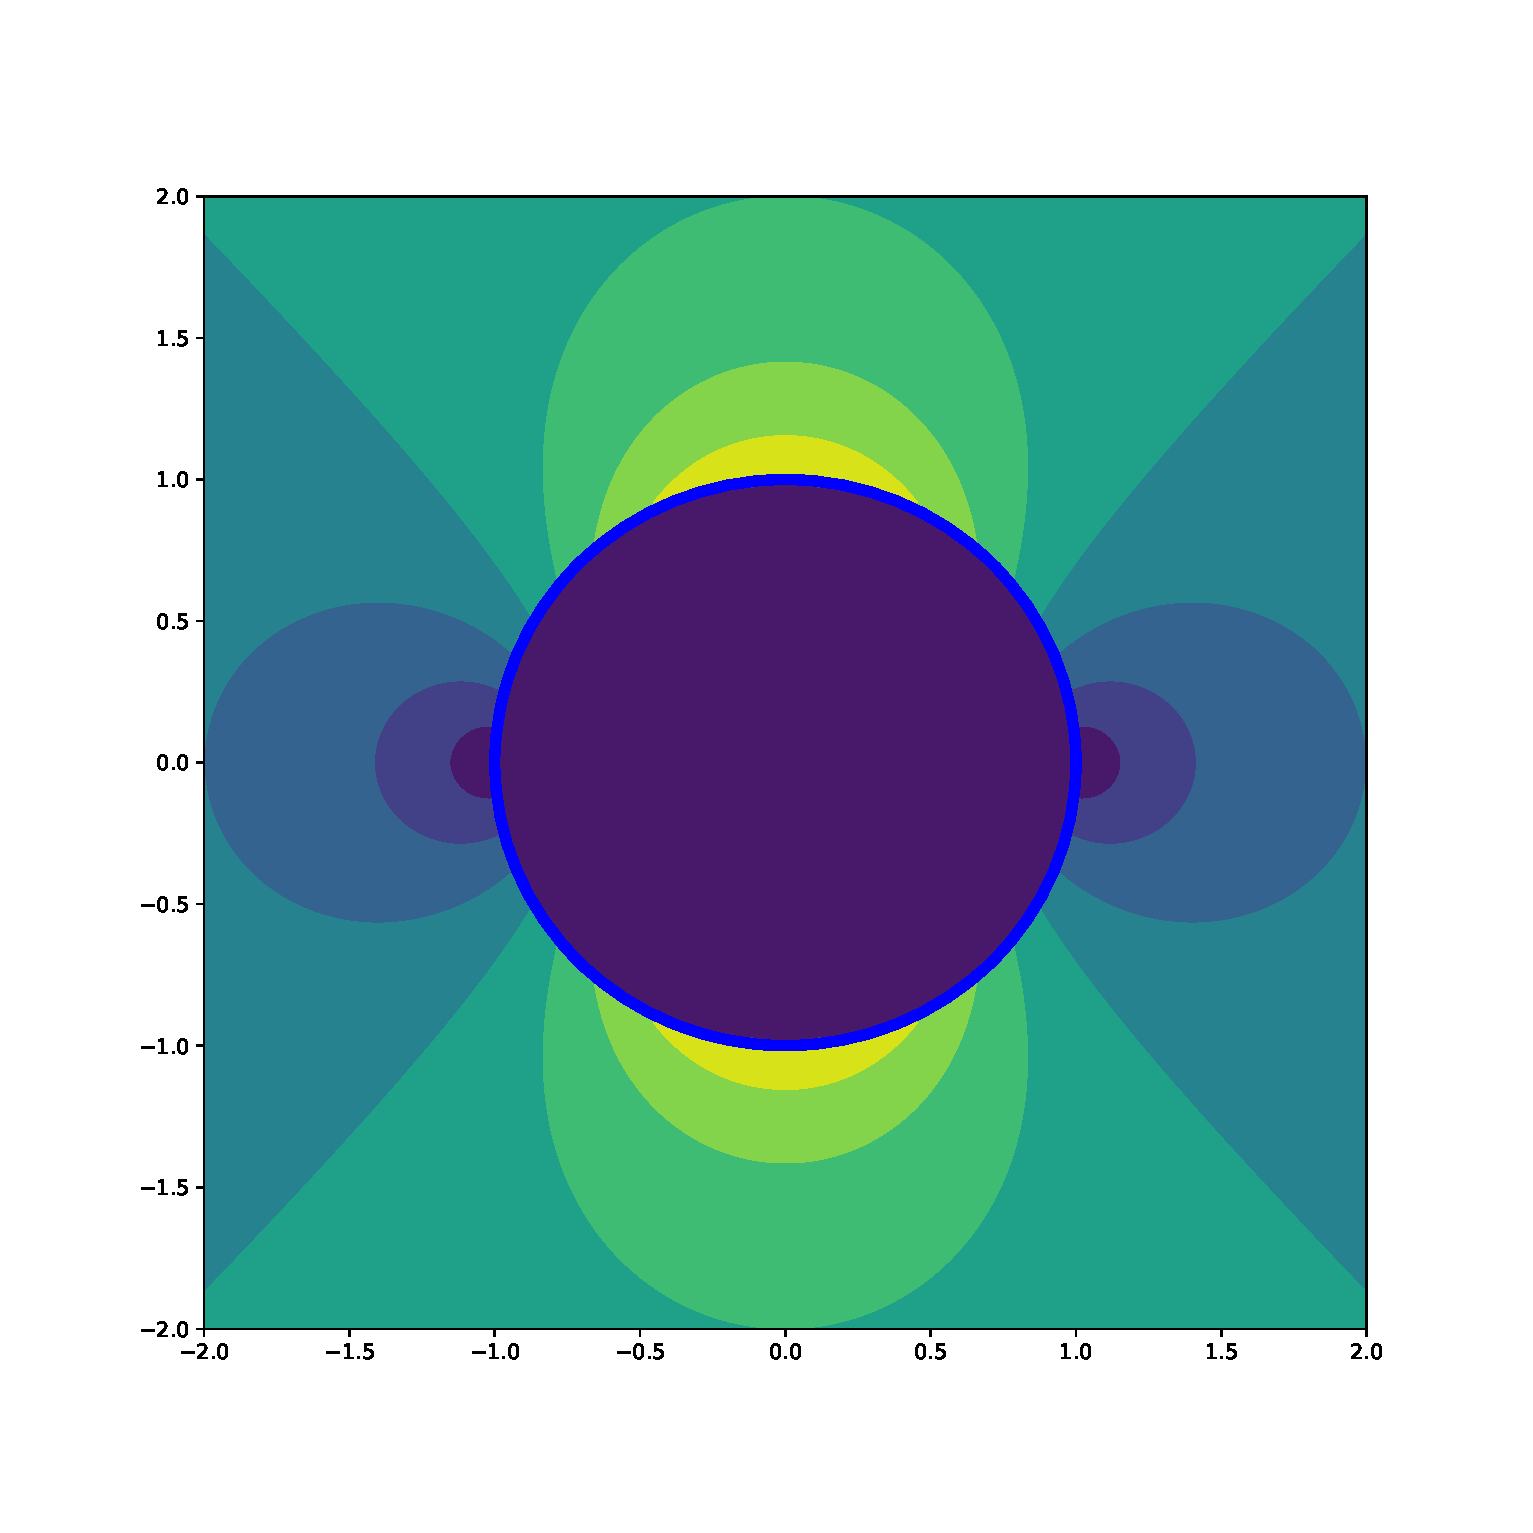
\includegraphics[width=0.4\linewidth]{figures/potential_flow_past_cylinder_vel}
  \caption{\label{fig:potential_flow_past_cylinder_vel}}
\end{figure}


\begin{figure}
  \centering
  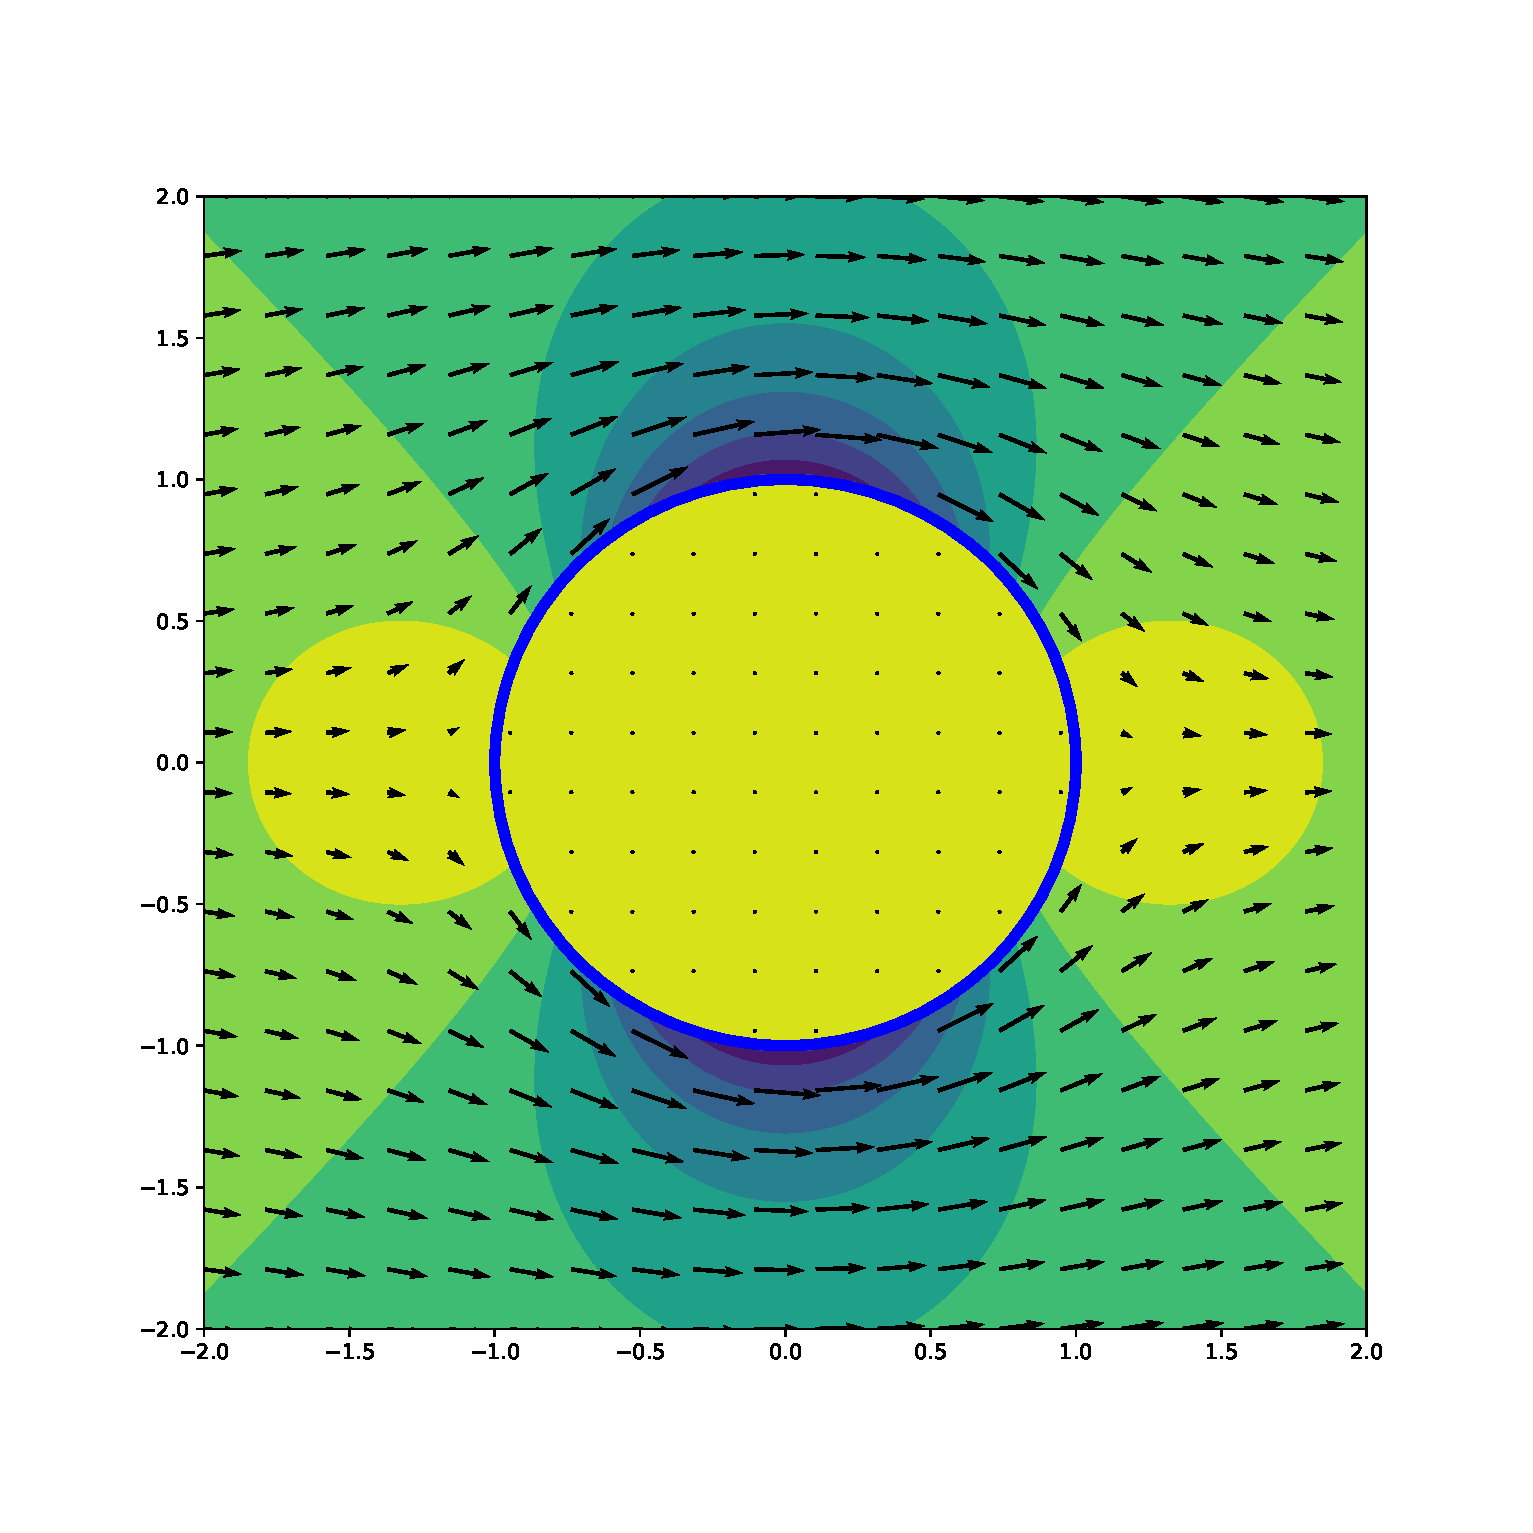
\includegraphics[width=0.4\linewidth]{figures/potential_flow_past_cylinder_vel_p}
  \caption{}%\label{fig:potential_flow_past_cylinder_vel}}
\end{figure}


The pressure field can be obtained from Bernoulli's principle:
\[
p= p_0 +  \frac{\rho}2  \left(u_0^2 - u^2 \right) ,
\]
and is plotted in
Fig. \ref{fig:potential_flow_past_cylinder_phi_p}. This Figure also
shows the potential field, to stress the difference between the
two. The velocity field does not simply ``goes from high to low
pressures'', except in those areas in which the two fields happen to
have similar gradients.

\begin{figure}
  \centering
  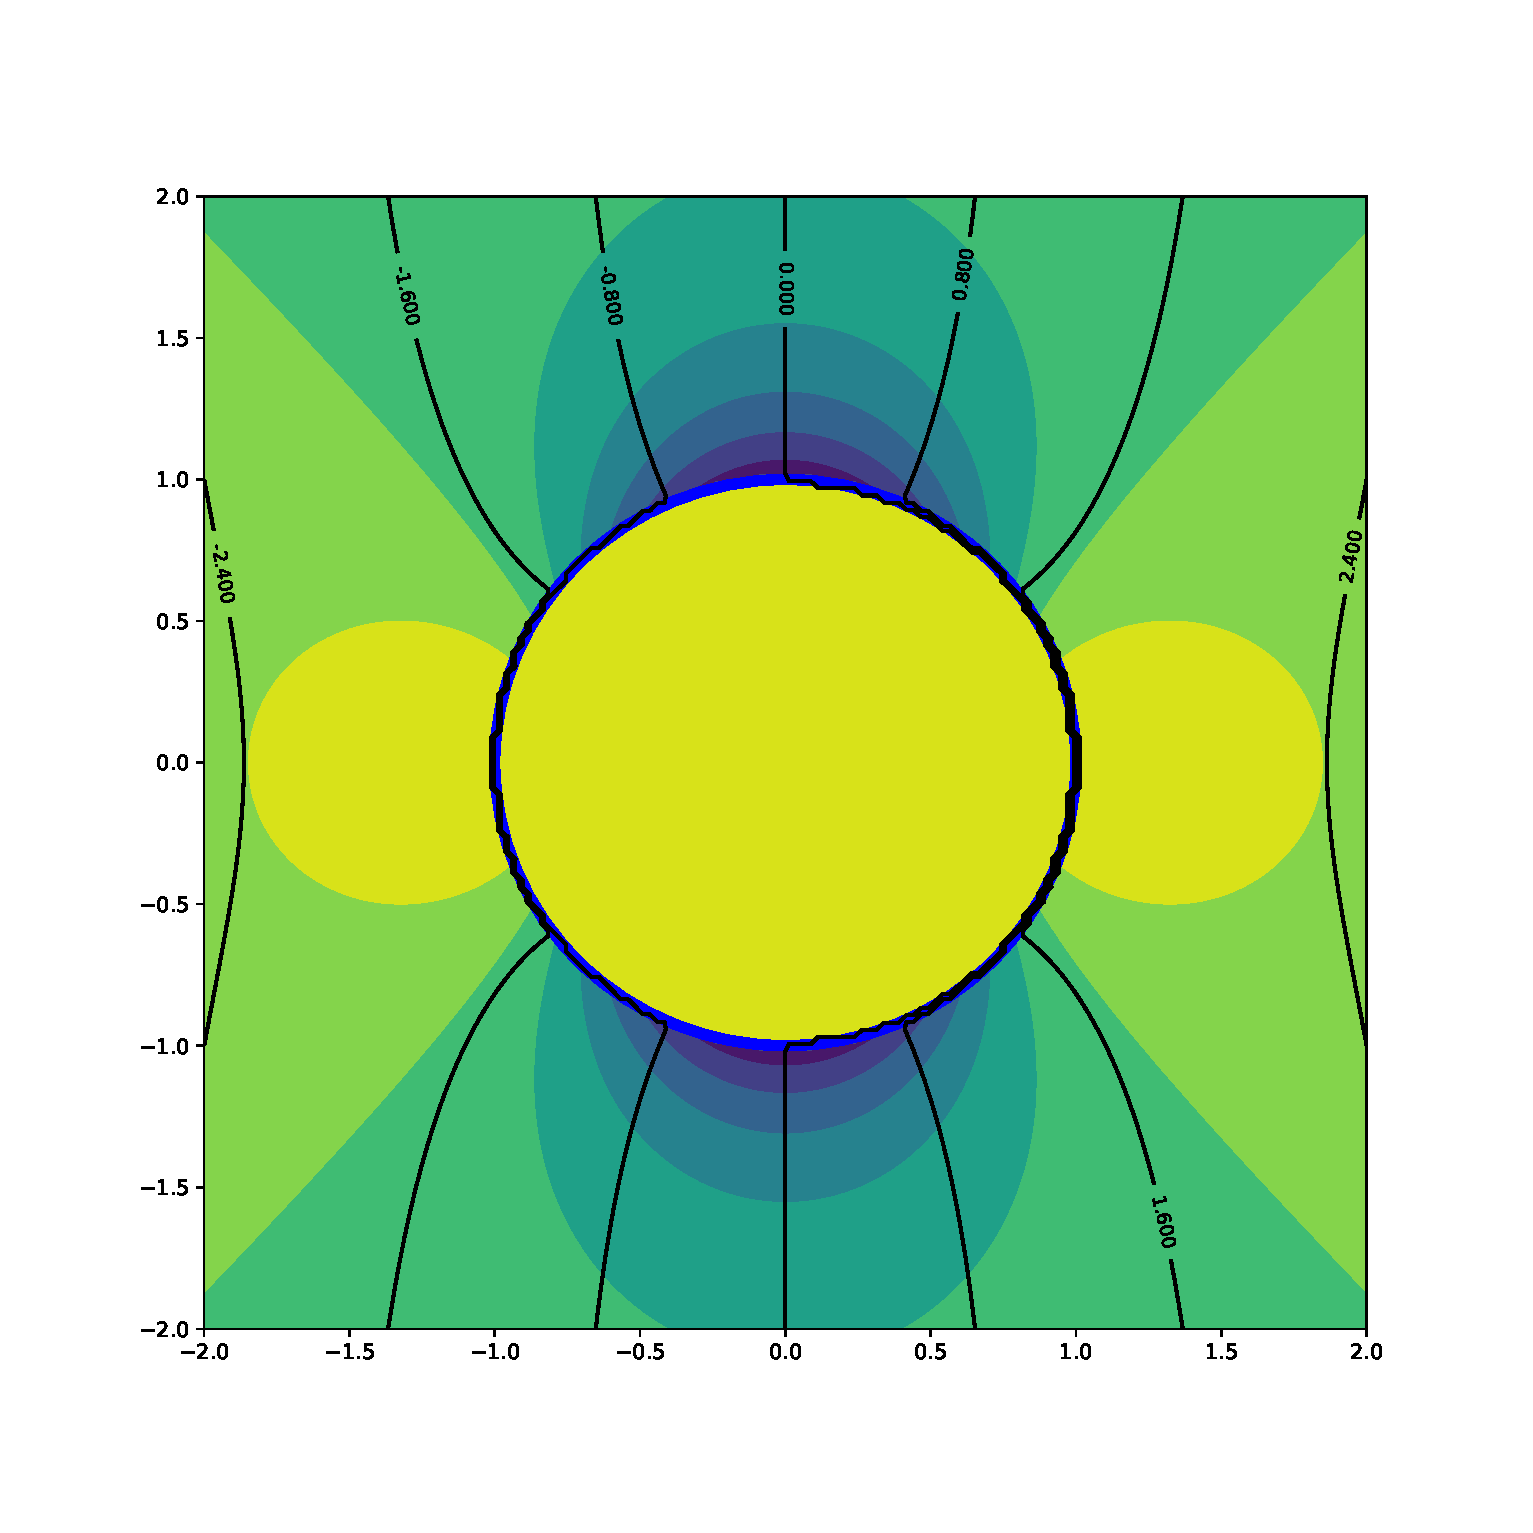
\includegraphics[width=0.4\linewidth]{figures/potential_flow_past_cylinder_phi_p}
  \caption{\label{fig:potential_flow_past_cylinder_phi_p}}
\end{figure}

The pressure field has a striking left-right symmetry. This of course
applied to its value at the surface. Since the pressure is the only
force this fluid may exert upon the cylinder, the consequence is that
the net force on it is exactly zero. The push it experiences towards
the right is exactly cancelled by the push back towards the
left. Therefore, the drag, which in this case is the net horizontal
force, is zero.

This striking result is known as d'Alembert's paradox, and marked a
historical chasm between theoretical fluid mechanics and applied
hydraulics. Indeed, the applied community could accept that the push
back may exist. Indeed, it had been hypothesized to be solely
responsible for objects moving even when not given a force in
Aristotelian physics. The effect is real, and is used regularly by
cyclist that may take advantage from it, by staying close to the back
of a moving vehicle. However, it is not acceptable to accept that it
should be exactly equal to the drag.

We now know that the crucial ingredient is the viscosity, which
manifests mathematically in a different boundary condition, such as
no-slip. This way, a real cylinder is dragged with the flow. We will
show later that it is easy to obtain the drag on a sphere in the limit
of high viscosity (a cylinder is not solvable due to another paradox,
as we will see.)

In case some mathematical justification is required, the pressure
at the surface on the cylinder is
\[
 p= p_0 + \frac12  u_0^2 \left(1 -  4   \sin^2(\theta) \right),
\]

Now, the drag is given by the net force in the $x$ direction. The
(vector) force due to pressure is:
\[
\mathbf{F} = \int_0^H \int_0^{2\pi}   p(\theta)  \bfn  R d\theta  dz ,
\]
where $p(\theta) \bfn \bhe_x R d\theta dz $ is the pressure force on a
differential surface of area $ R d\theta dz$. Now, the drag will be
its projection on the horizontal axis:
\[
D= \mathbf{F} \cdot \bhe_x = \int_0^H \int_0^{2\pi}
p(\theta) \cos(\theta) R d\theta dz .
\]
The integral is zero, since it consists of two terms. The first one
involves constant term. Of course, a constant pressure exerts no net
force, and mathematically:
\[
 \int_0^{2\pi} C \cos(\theta) d\theta = C  \int_0^{2\pi}  \cos(\theta) d\theta = 0 .
\]

The other term involves a $sin^2$ term. Now, this integral is also
zero:
\[
 \int_0^{2\pi}  \cos(\theta)  \sin^2(\theta) d\theta = 0 .
\]
qThe reason is that $\sin^2$ may be written as another constant term
and a term proportional to $\cos(2\theta)$. (To be precise,
$\sin^{2}\theta ={\frac {1-\cos(2\theta )}{2}}$.) Cosines form an
orthogonal basis: an integral of two different cosines over one period
will be zero. Unless they are the same cosine, when the integral is
$\pi$. To be precise, for integer $m$ and $n$:
\[
\frac{1}{2\pi} \int_0^{2\pi}  \cos(m \theta) \cos(n \theta)  d\theta = 
\begin{cases}
0 \quad \text{if } m\ne n \\
\frac12 \quad \text{if } m = n 
\end{cases} .
\]
(It is more elegant to divide by $2\pi$ to express the integral as a
mean value.) In fact, the previous result about the constant pressure
is a particular case in which $m=0$.

It is also interesting that such an integral involving a sine and a
cosine is always zero. This shows that the lift is always null:
\[
L= \mathbf{F} \cdot \bhe_x = \int_0^H \int_0^{2\pi}
p(\theta) \sin(\theta) R d\theta dz = 0
\]



\subsection{Streamlines}

For steady 2D flow, it is very convenient to introduce the stream
function $\psi$. It is defined such that its contour lines produce the
streamlines \index{streamline}, i.e. the lines the fluid particles
trace as they move. Upon some reflection, this means that its gradient
should always be perpendicular to the velocity:
\begin{equation}
  \label{eq:stream_perp_to_u}
  \bfu \cdot \nabla\psi = 0 .
\end{equation}
In steady flow, this means $d\psi/dt=0$, so the value of $\psi$ is
carried with the flow. This is at variance with the potential, whose
gradient is parallel to the velocity (it is indeed, the velocity
itself). Thus $\phi$ and $\psi$ are orthogonal functions, in the sense
that their gradients are.

The streamlines are important to visualize flows, in much the same way
as Faraday's field lines are for electromagnetic fields
(mathematically, they are equivalent). In computational fluid
dynamics, they are customarilly computed and plotted, by ``seeding''
points and integrating their motion following the velocity field.  A
fine point is that for unsteady flow, these streamlines are in general
different from the actual trajectories of fluid particles, which are
called ``pathlines'' \index{pathline}.


For steady flow, it is often convenient to define a vector potential
\index{vector potential} in much the same way as it is done for the
magnetic field in electromagnetism:
\begin{equation}
  \label{eq:vector_potential}
  \bfu = \nabla\times \bfA .
\end{equation}

The resulting velocity field will always be incompressible, since the
divergence of a curl is zero.

In the case of 2D, the choice for this vector potential is
\begin{equation}
  \label{eq:A_psi_2D}
  \bfA = \psi(x,y) \bhe_z ,    
\end{equation}
perpendicular to the plane, but dependent on the in-plane
coordinates. With this expression,
\begin{align*}
  u_x &=  \frac{\partial \psi}{\partial y} \\
  u_y &= -\frac{\partial \psi}{\partial x} ,
\end{align*}
and it is easy to check that this stream function indeed traces
stream-lines, since it complies with \ref{eq:stream_perp_to_u}.

In cylindrical coordinates \cite{wiki:del},
\begin{align*}
u_r &= \frac1r \frac{\partial \psi}{\partial \theta} \\
u_\theta &=   - \frac{\partial \psi}{\partial r} .
\end{align*}


\subsection{Streamlines around the cylinder}

With tha latter expression for the stream function, and from our
results for the velocity field, the $\psi$ field is found to be
\[
\psi = u_0 \left( r-{\frac {R^{2}}{r}}\right)\sin \theta .
\]
This method, of course, is working backwards from the known
solution. It is also possible to derive the velocity field from the
fact that $\psi$ satisfies Laplace's equation, plus the appropriate
boundary conditions, in a manner very similar to what has been done
for the potential (see Exercise \ref{ex:u_from_psi_cylinder}).

The contour lines of this field are shown in
Fig. \ref{fig:potential_flow_past_cylinder}.

\begin{figure}
  \centering
  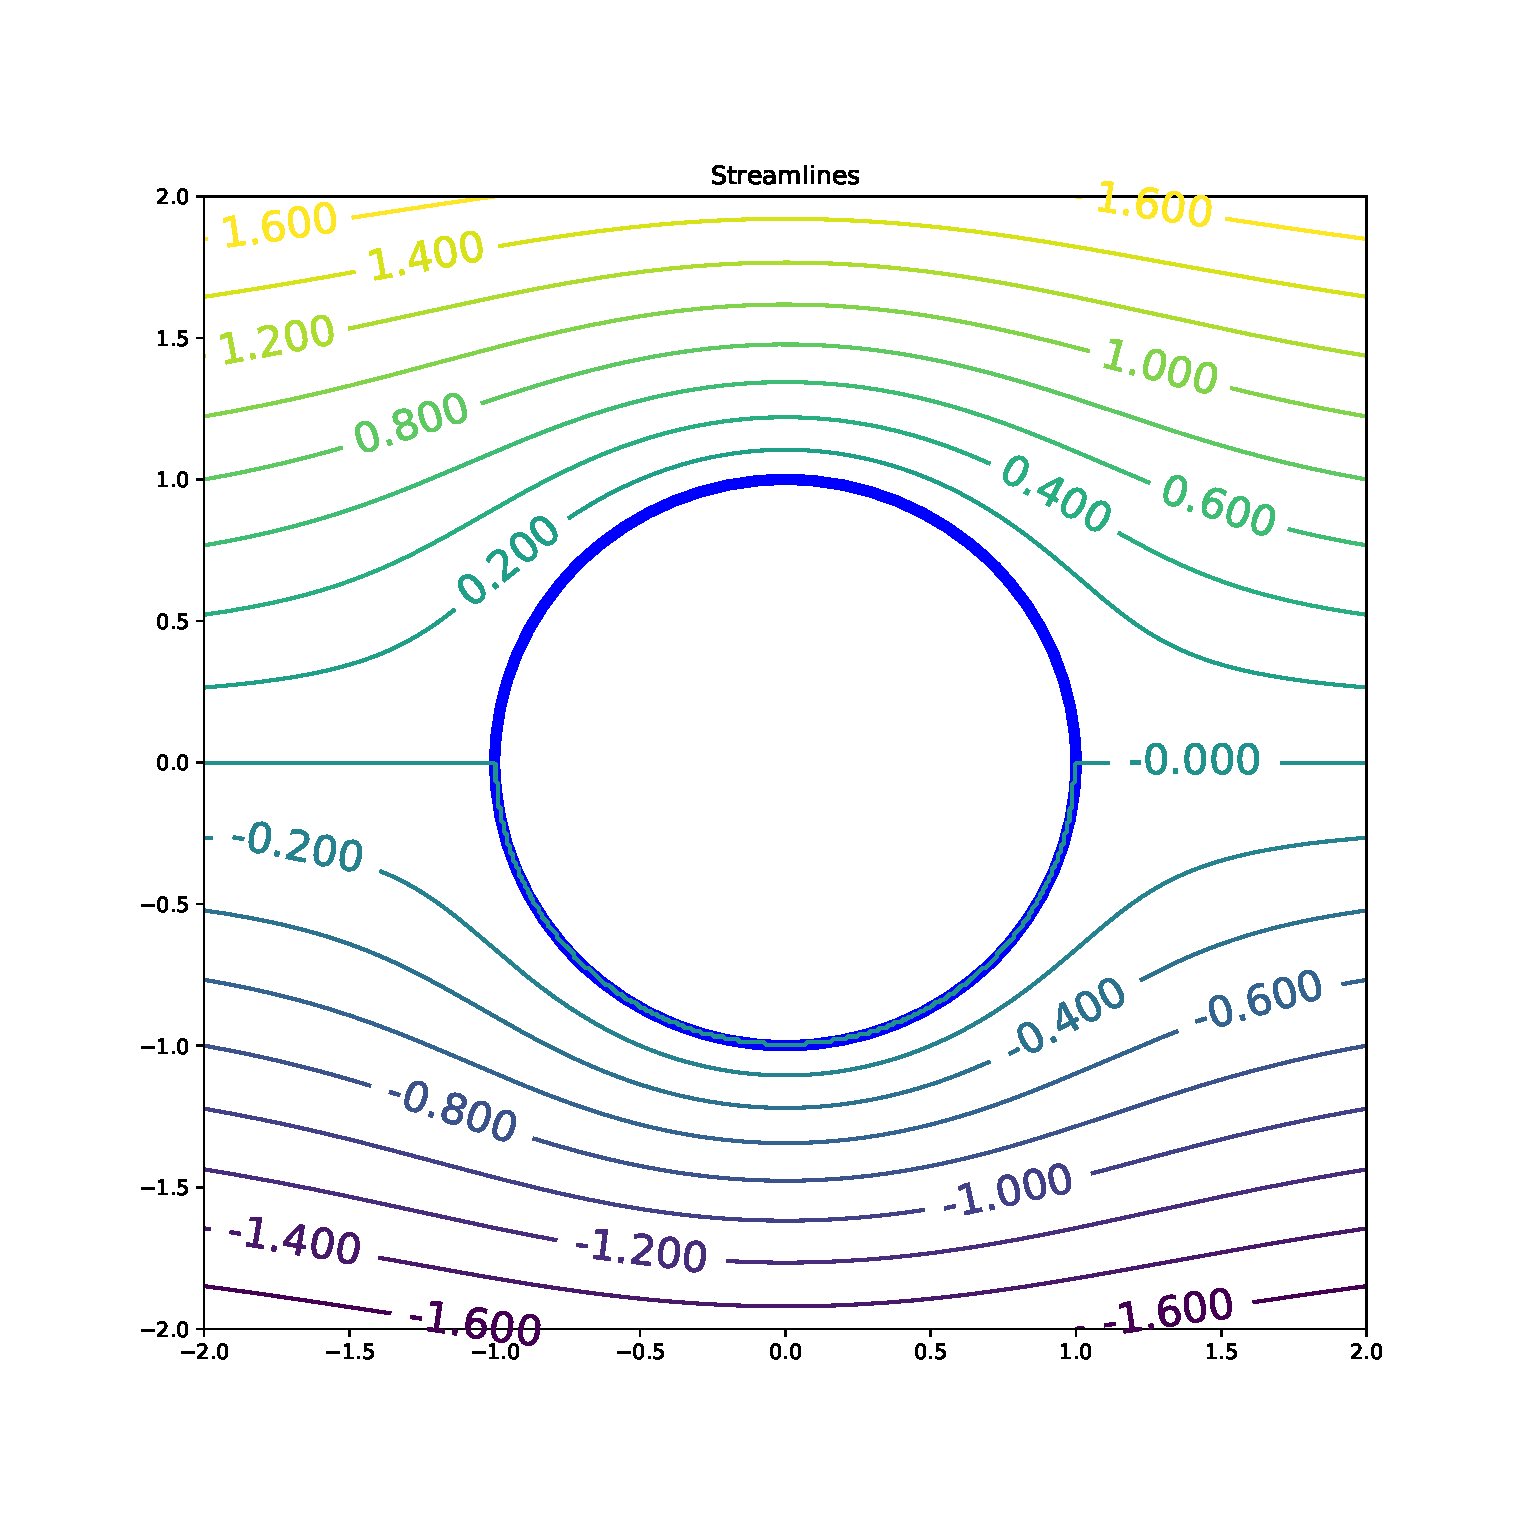
\includegraphics[width=0.4\linewidth]{figures/potential_flow_past_cylinder}
  \caption{\label{fig:potential_flow_past_cylinder}}
\end{figure}

Interestingly, the $\psi$ field is also a solution of Laplace's
equation, $\nabla^2 \psi=0$, as can be checked explicitely --- but
also from the identity for the curl of the curl
\cite{wiki:Vector_calculus_identities}:
\begin{equation}
  \label{eq:curl_of_curl}
  \nabla \times \left(\nabla \times \bfA \right)=
  \nabla (\nabla \cdot \mathbf {A} )-\nabla^2\bfA .
\end{equation}

Then, since the velocity field is curl-free:
\[
   \nabla \times \bfu = 0 =
   \nabla (\nabla \cdot \mathbf {A} )- \nabla^{2}\mathbf {A} =
   - \bhe_z \nabla^{2} \psi,
\]
where we use the fact that the $\bfA$ field of \ref{eq:A_psi_2D} is
divergence-free.


There is also the intriguing fact that we may write
\[
\phi = u_0 \Re \left( z  + \frac{R^2}{z} \right) ,
\]
where $z=r e^{i\theta}$ is the complex number related to the $r$ and
$\theta$ coordinates. Then,
\[
\psi = u_0 \Im \left( z  + \frac{R^2}{z} \right) .
\]
%
I.e. both fields are the real and imaginary part of the same complex
function:
\[
f(z) = u_0 \left( z  + \frac{R^2}{z} \right)
\]

This is no coincidence, but a consequence of Cauchy-Riemann
equations: the real and imaginary part of a complex function are
harmonic (i.e. they satisfy Laplace's equation) and orthogonal. To be
more precise, the complex function must be analytic. The later
requirement is pretty general: it means the function must be
single-valued and and must have a derivative everywhere. The reader
may worry about the origin and the $1/z$ function. This is, however,
outside our domain, which ends when $r>R$. However, the fact that our
domain has this ``hole'' in it has some consequences, as we will see
next.


\subsection{Circulation and lift}

It turns out that, despite our previous claims of having found the
solution to the problem, this is not a unique solution%
\footnote{This is because our domain has a hole in it. Technically, it
  is not simply-connected. This means there is an additional parameter
  to fix the most general solution. This is called the ``winding
  number'', and is basically this section's $\Gamma$.}.
%
The most general one is given by
\[
 f(z) = u_0 \left( z + \frac{R^2}{z} \right)
 + \frac{i \Gamma}{2\pi} \log z \qquad
 \phi=\Re(f) \quad
 \psi=\Im(f) .
\]
I.e. we may add an additional term which is also analytic. The $i
\Gamma/(2\pi)$ factor is chosen for convenience, as will become
clear. Both $\phi$ and $\psi$ are still harmonic and orthogonal, since
$\log(z)$ is analytic. Notice $i \log(z)= i \log(r) - \theta$, so
$\phi$ contains a term that is just the polar angle, while $\psi$ will
include a $\log(r)$ term.

The resulting velocity field still complies with the boundary
conditions, since the resulting velocities:
\begin{align}
u_r     &=   u_0  \left[ 1 - \left( \frac{R}{r}\right)^2 \right] \cos(\theta) \\
u_\theta &=   u_0  \left[ 1 + \left( \frac{R}{r}\right)^2 \right] \sin(\theta) +\frac{\Gamma}{2\pi r} 
\end{align}
have an additional term which dies away far from the cylinder, while
the no-trespass condition at the surface is still respected (since the
radial velocity does not change at all).

The name of $\Gamma$ is ``circulation'', since
\[
\Gamma = \oint_C \bfu\cdot d\mathbf{l}
\]
for any contour around the cylinder \footnote{This makes the velocity
  field non-conservative, which is again allowed due to the domain
  being not simply-connected.}.

At the surface of the cylinder,
\[
u= u_\theta =   u_0  2 \sin(\theta) +\frac{\Gamma}{2\pi R} .
\]
The stagnation points then move away from their positions, to points given by
\[
\sin(\theta_\mathrm{st})  = \frac{\Gamma}{4\pi R u_0} .
\]
This has two solutions, of course, as long as the right-hand side is
between $-1$ and $1$. For values below or above, the points coalesce
into a single stagnation point that is outside the cylinder.

\begin{figure}
  \centering
  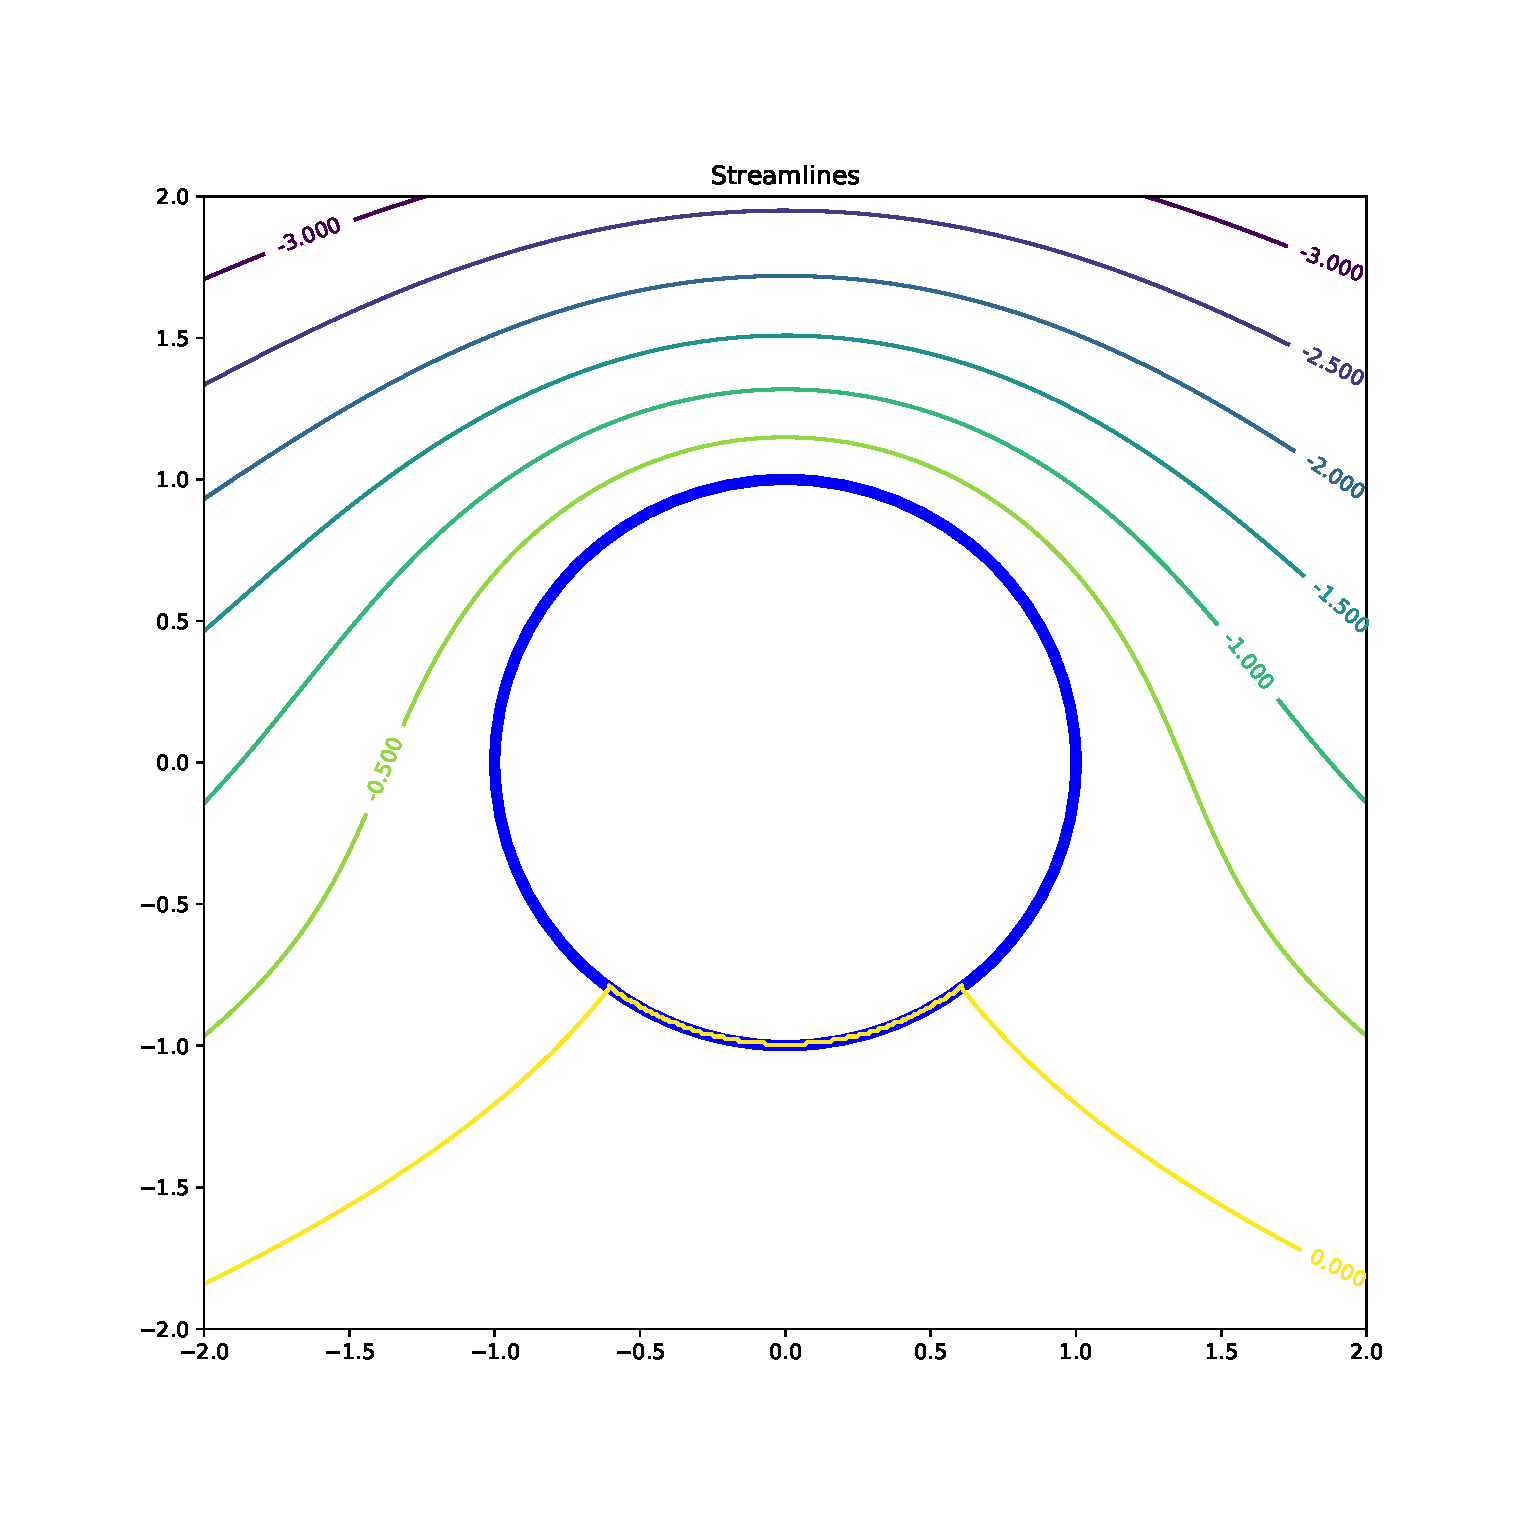
\includegraphics[width=0.4\linewidth]{figures/potential_flow_past_cylinder_rotating}
  \caption{\label{fig:}}
\end{figure}


This new velocity field does not solve d'Alambert's paradox, but it
does provide a lift, since the pressure at the surface is
\[
p= p_0 + \frac{\rho}2   \left(u_0^2 -  \left[ 2  u_0 \sin(\theta) - \frac{\Gamma}{2\pi R} \right]^2 \right) =
\ldots  2 \rho u_0   \frac{\Gamma}{2\pi R} \sin\theta ,
\]
where we single out the only term that can produce a contribution to the lift.

Now,
\[
L= \mathbf{F} \cdot \bhe_x = \int_0^H \int_0^{2\pi}
p(\theta) \sin(\theta) R d\theta dz =
2 L  \rho u_0  R  \frac{\Gamma}{2\pi R}   \int_0^{2\pi}  \sin^2(\theta) d\theta =
 H \rho u_0   \Gamma .
\]
Therefore, the lift per unit length is $L/H= \rho u_0 \Gamma$. It is
interesting that heavier fluids, high speeds and high $\Gamma$ produce
higher lift forces.

It turns out that this result for the lift is quite general, at least
for these kind of potential flows. It is known as the Kutta-Joukowski
Lift Theorem, and has been used for decades in aeronautics. The idea
is to map our solution for a cylinder to another, more wing-like,
shape, by some conformal transformations. These transformations, or
``mappings'', preserve the harmonicity of functions --- hence the
transformed $\phi$ and $\psi$ will still be solutions of Laplace's
equation. Historically, the best known mappings are the Joukowsky
K\'arm\'an–Trefftz transforms.

For a plane wing, it makes sense to relate circulation and lift, since
this captures, in a way, the fact that the velocity is higher at the
top of the wing, lower below, so the net circulation is non zero. (Of
course, this cannot hold right at the surface of an actual wing, since
the velocity there will be zero. But this can be measured somewhat
further away, beyond a boundary layer.) For a cylinder, this makes
little sense, but this picture is sometimes used to explain the Magnus
effect. This causes a rotating cylinder to bend as it moves across a
fluid. This is used (for spheres) in sports, such as tennis, golf and
football. Also, for cylinder-like rotors in ``rotor ships,'' which use
the Magnus effect for propulsion.

As an aside, if we move along with the plane, or ship, we will not see
those velocity fields. The horizontal component should be avoided in
every equation, and the resulting velocity looks different. This is
shown in Fig. \ref{fig:potential_flow_past_cylinder_moving}, for the
flow past a cylinder with and without circulation. It is seen that,
for an observoer moving with the cylinder, the surrounding fluid is
pushed from the fore, and moved around towards the aft (where it
pushes our vehicle, magically making our journey a costless one!).

\begin{figure}
  \centering
  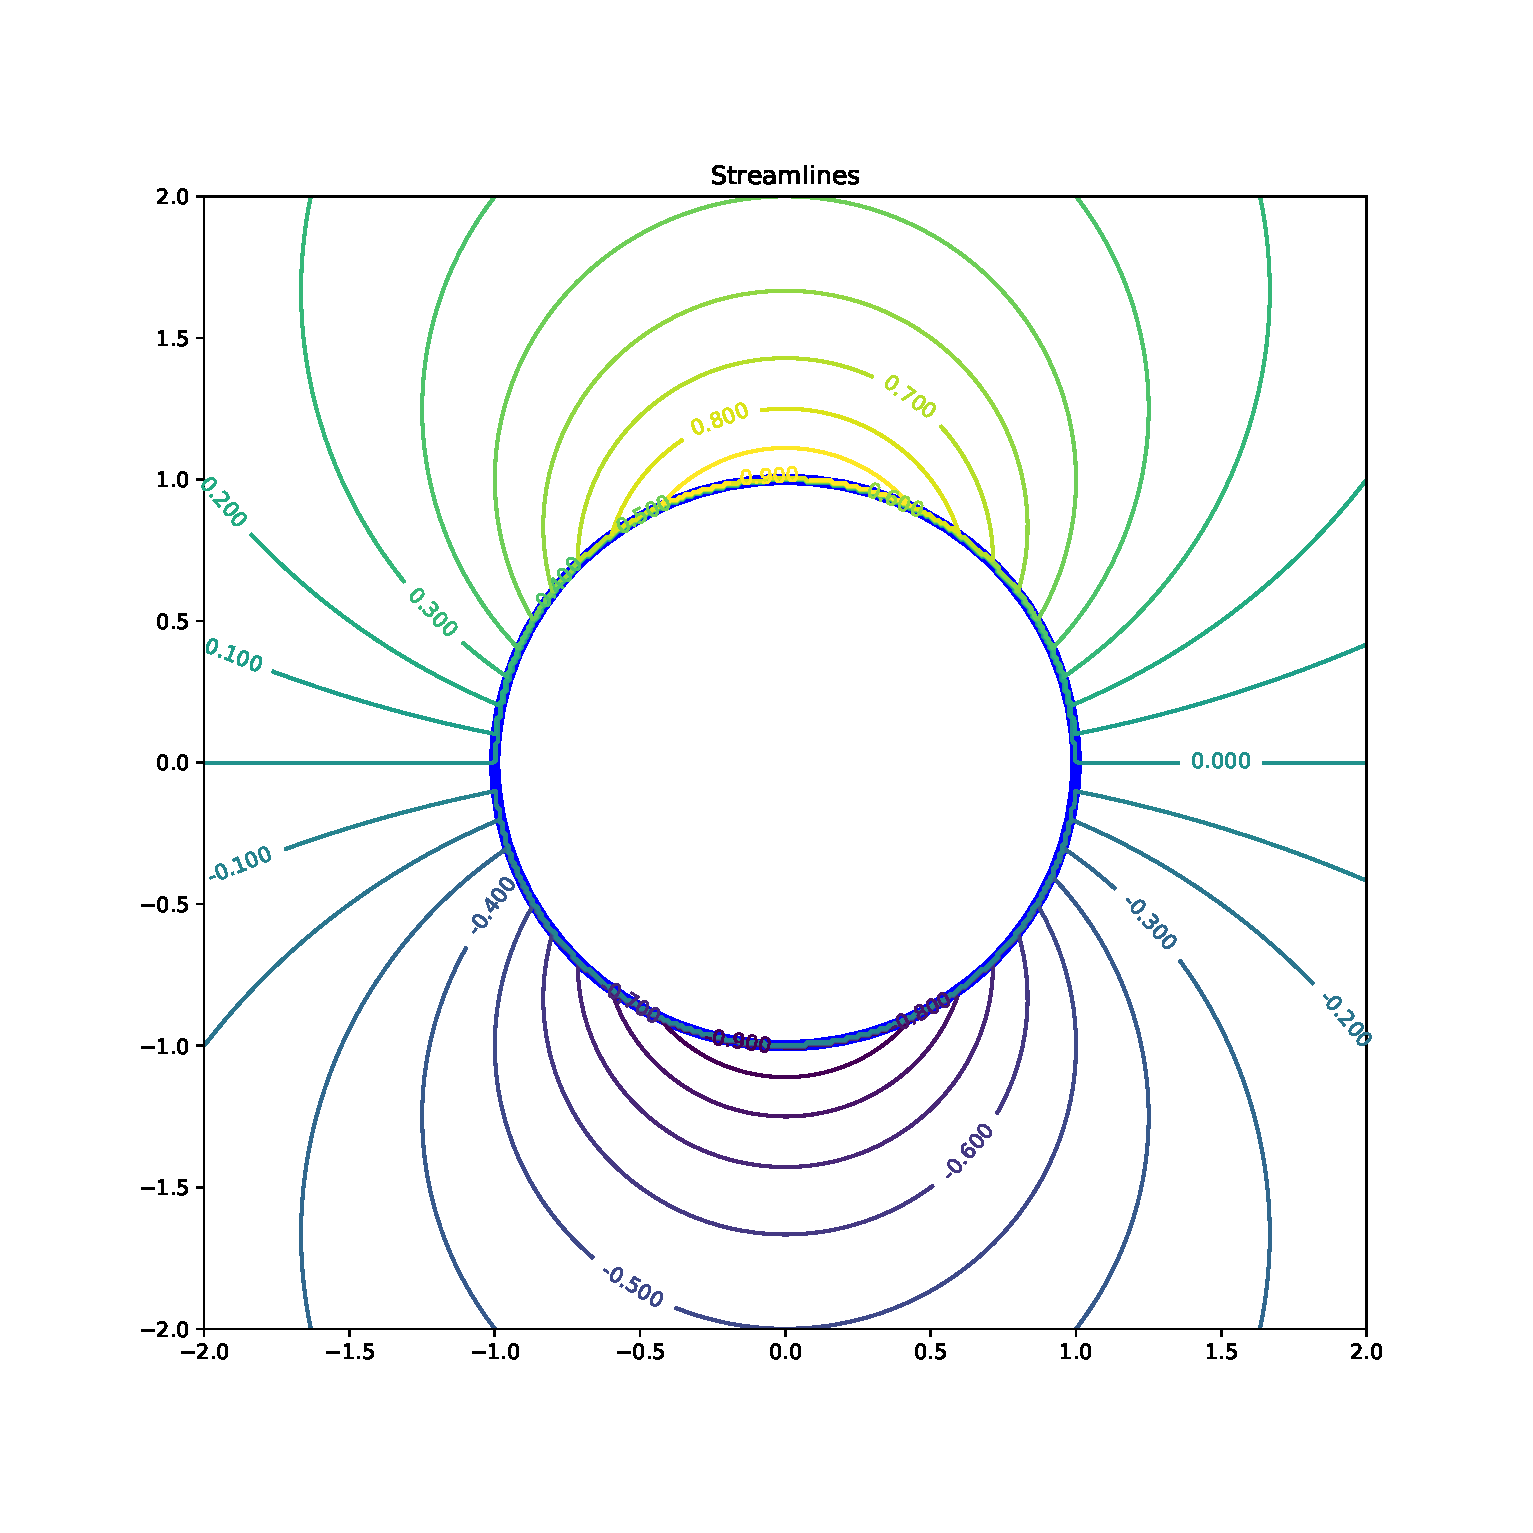
\includegraphics[width=0.4\linewidth]{figures/potential_flow_past_cylinder_moving}
  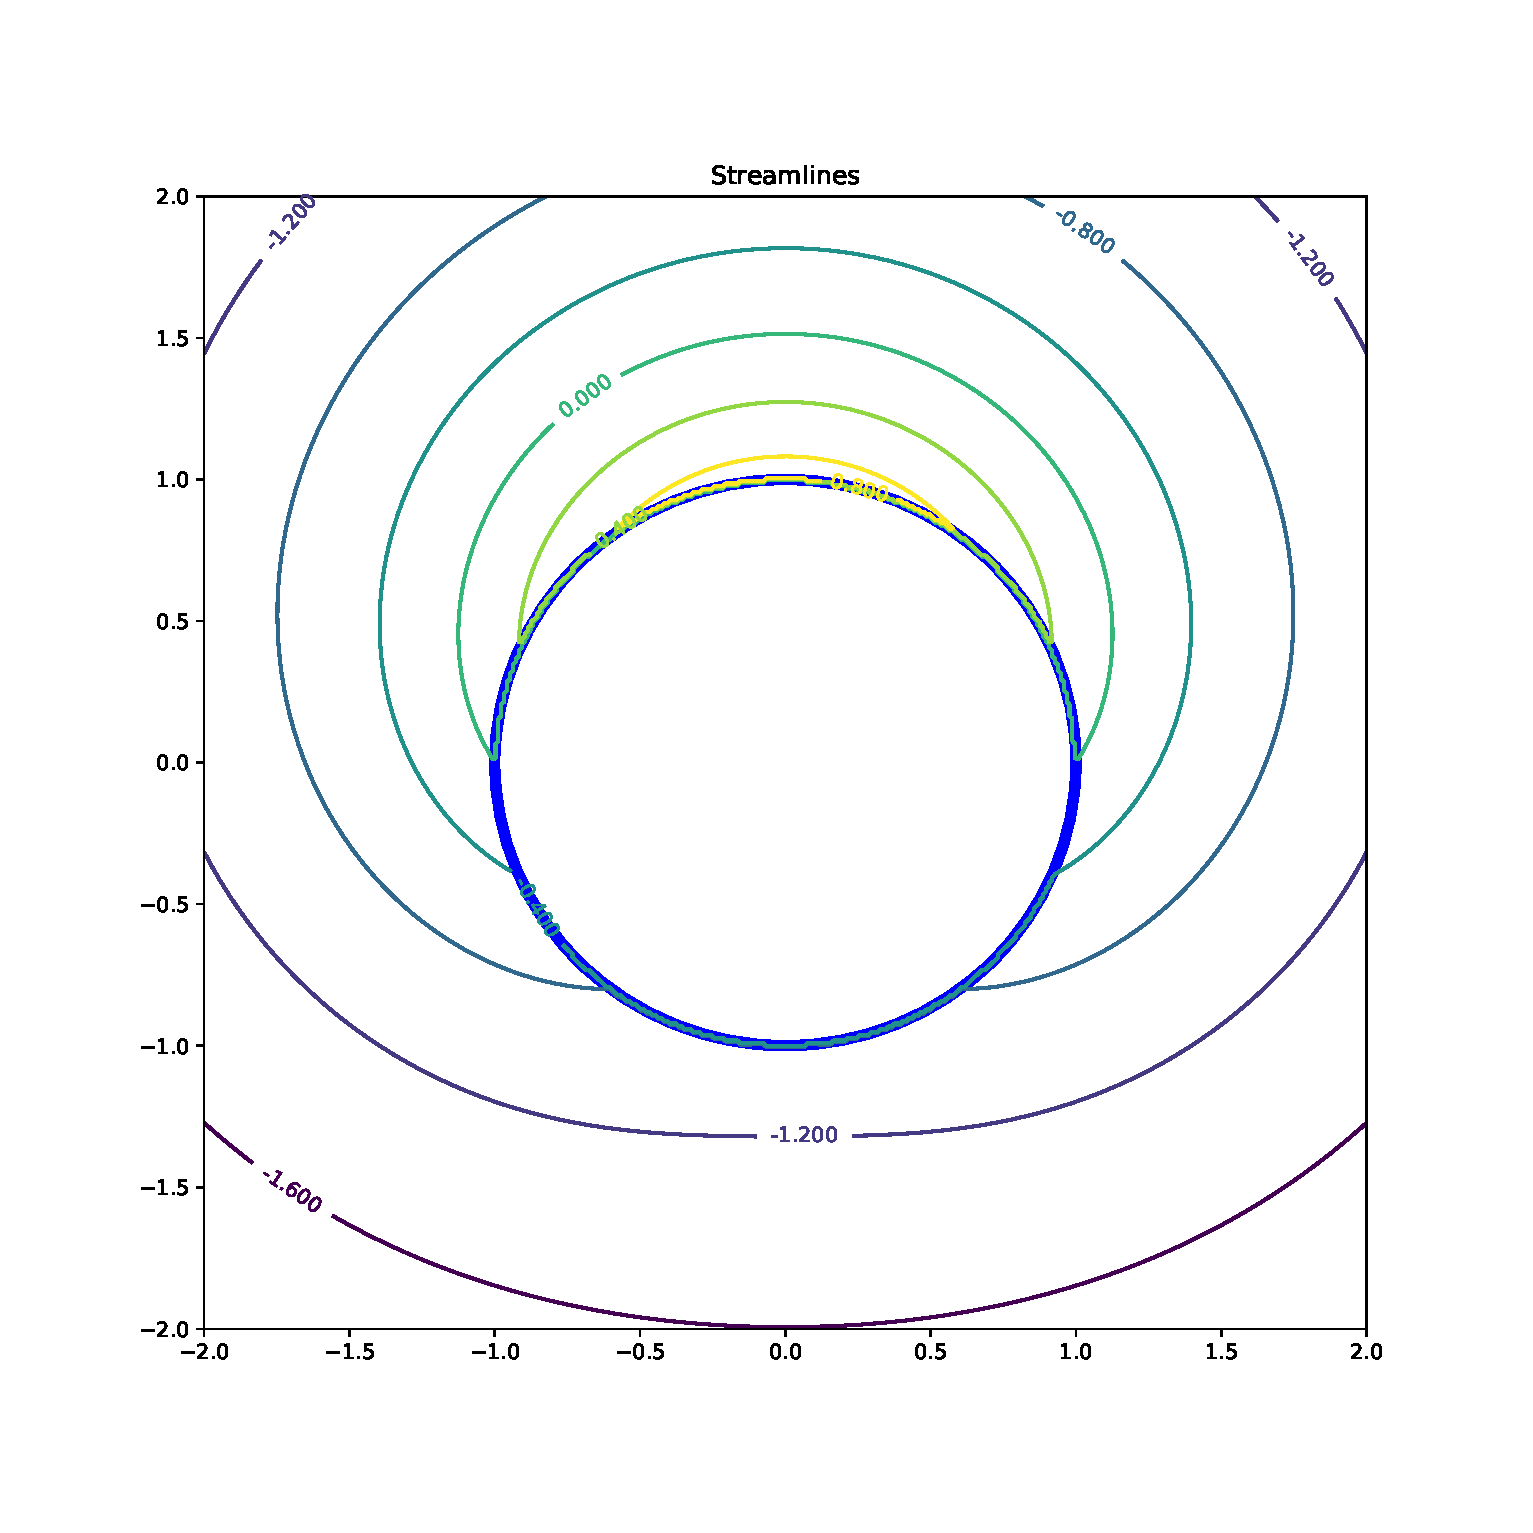
\includegraphics[width=0.4\linewidth]{figures/potential_flow_past_cylinder_rotating_moving}
  \caption{\label{fig:potential_flow_past_cylinder_moving}}
\end{figure}


\subsection{Flow past a sphere}

With the same assumption of potential flow as in the cylinder, the
axisymmetric flow past a sphere may be tackled by using the potential,
which should satisfy Laplace's equation, plus these boundary
conditions:
\[
  \phi (r\to \infty) \to u_0 z = u_0 r \cos\theta \qquad
  u_r(r=R) =\left. \frac{\partial \phi}{\partial r} \right|_{r=R} = 0 .
\]
Spherical coordinates \index{spherical coordinate system} are used:
$r$ is the distance to the origin, $\theta$ is the polar angle (angle
with the $z$ axis), and the azimuthal angle (angle around the $z$
axis), here absent due to symmetry, is $\phi$ %.
\footnote{This naming convention is the most common in physics, and is
  pecified by ISO standard 80000-2:2009, and earlier in ISO 31-11
  (1992). However, the name of the two angles is often reversed,
  specially in mathematics. The advantage of the latter is that
  $\theta$ then retains the same name as in 2D polar coordinates.}.


Similarly to the cylinder, let us try a function
\[
\phi =  \left( u_0 r  + f(r) \right) \cos(\theta)  .
\]

By using the expression of the Laplacian in spherical coordinates
\cite{wiki:del}, we soon come to the conclusion that $f(r)= A/r $ in
order Laplace's equation be satisfied. This function also vanishes as
$r$ gets large, as it should. With the no-trespassing condition for the
velocity the value of $A$ may be found out.

The final result is
\[
  \phi(r,z) = u_0 r
  \left[
    1 +
    \frac12 \left( \frac{R}{r}\right)^3
  \right] \cos\theta .
\]
From its gradient we get the velocity field:

\begin{align*}
u_r &=  u_0
  \left[
    1 -
      \left(\frac{R}{r}\right)^3
  \right] \cos\theta \\
u_\theta &=  -u_0
  \left[
    1 + \frac12
      \left(\frac{R}{r}\right)^3
  \right] \sin\theta
\end{align*}


\subsubsection{Streamlines past a sphere}

For axisymmetric flows, streamlines may be defined on a plane, since
the resulting flow does not depend on the azimuthal angle (the angle
around the axis of symmetry, which is $z$). However, these are not 2D
flows, and the equations are more involved.

In this case, the velocity field depends only on the other two
coordinates. In spherical coordinates,
\[
  \bfu = \bfu(r,\theta) .
\]

The vector potential is still chosen as ``perpendicular'' to the other
two coordinates. In spherical coordinates:
\[
  \bfA = A \bhe_\phi ,
\]
i.e. it is purely azimuthal. It is also divergence-free, so that is
satisfies Laplace's equation for a curl-free flow.

However, the choice of $A=\psi$ does \emph{not} result in the correct
stream-line behavior of Eq.  \ref{eq:stream_perp_to_u}. The following
choice, however, does:
\begin{equation}
  \label{eq:Stokes_stream_spherical}
  \bfA = \frac{\psi(r,\theta)}{r \sin\theta } \bhe_\phi .    
\end{equation}
%
This $\psi$ is called ``Stokes' stream function''\index{Stokes' stream
  function}, but there is no fundamental difference with the usual,
2D, stream function.

The resulting velocity field for spherical coordinates is then found
to be
\begin{equation}
  \label{eq:u_from_psi_spherical}
  \begin{split}
    u_r     &=  \frac1{r^2 \sin\theta} \frac{\partial \psi}{\partial \theta} \\
    u_\theta &= -\frac1{r   \sin\theta} \frac{\partial \psi}{\partial r}
  \end{split}
\end{equation}

For completeness, in cylindrical coordinates the appropriate
expression is
\[
  \bfA = \frac{\psi(\rho, z)}{ \rho } \bhe_\phi ,
\]
where $\rho$ is the distance to the $z$ axis. The
resulting velocity field is
\begin{equation*}
  \begin{split}
    u_\rho   &= - \frac1{\rho} \frac{\partial \psi}{\partial z} \\
    u_z     &=   \frac1{\rho} \frac{\partial \psi}{\partial \rho}
  \end{split}
\end{equation*}


For the flow around a sphere, the resulting stream function is then
found to be
\begin{equation}
  \label{eq:potential_sphere_stream}
  \psi(r,\theta) = \frac12 u_0 r^2
  \left[
    1 -
    \left(\frac{R}{r}\right)^3
  \right] \sin^2\theta .
\end{equation}
Again, this is found by working backwards from the known solution.
See Exercise \ref{ex:u_from_psi_spher}) to derive the velocity field
from $\psi$.

In Fig. \ref{fig:potential_streamlines_sphere} these streamlines are
plotted. The corresponding streamlines for the flow as seen from the
sphere are in Fig. \ref{fig:potential_streamlines_moving_sphere}.

\begin{figure}
  \centering
  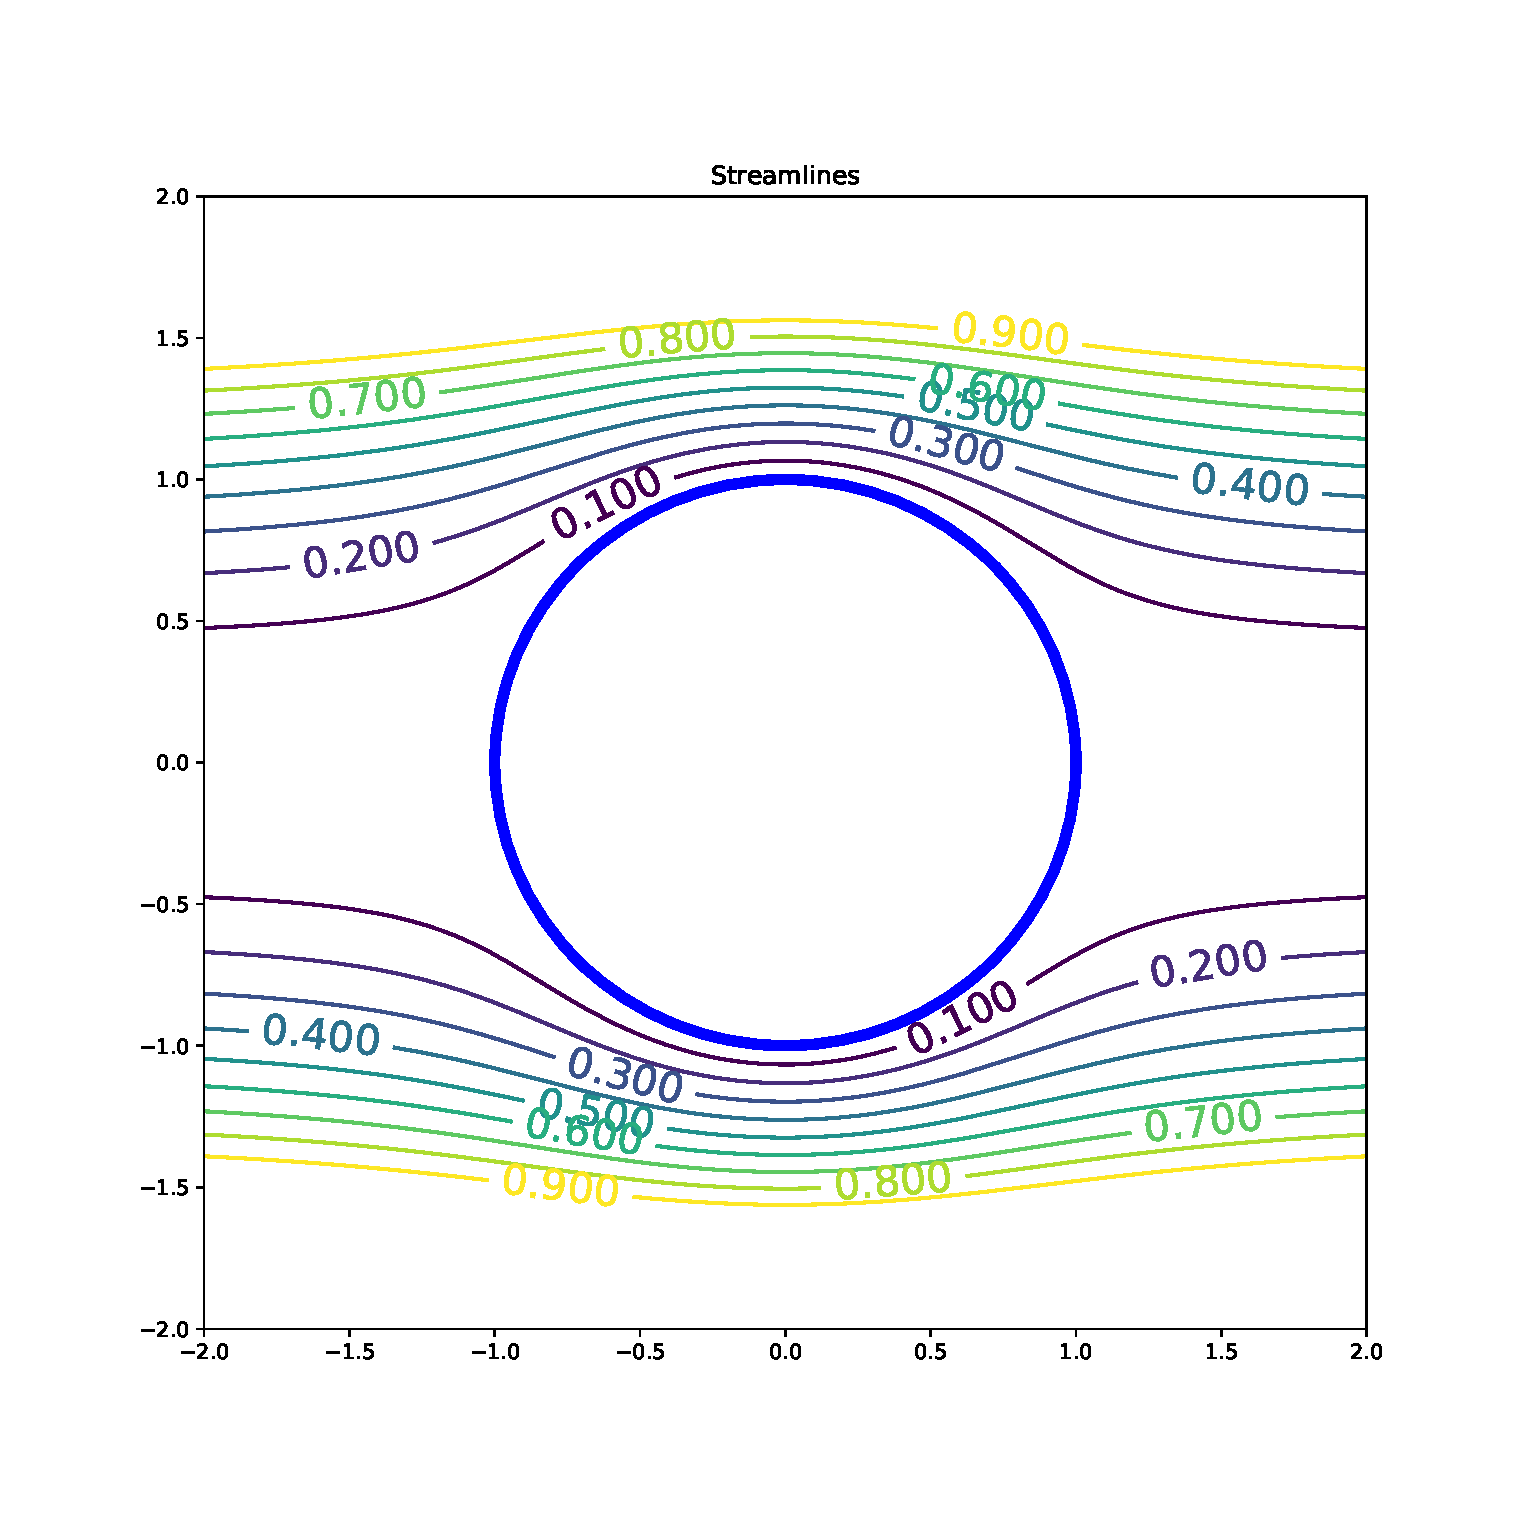
\includegraphics[width=0.4\linewidth]{figures/potential_flow_past_sphere}
  \caption{\label{fig:potential_streamlines_sphere} Streamlines of
    the potential flow past sphere}
\end{figure}



\begin{figure}
  \centering
  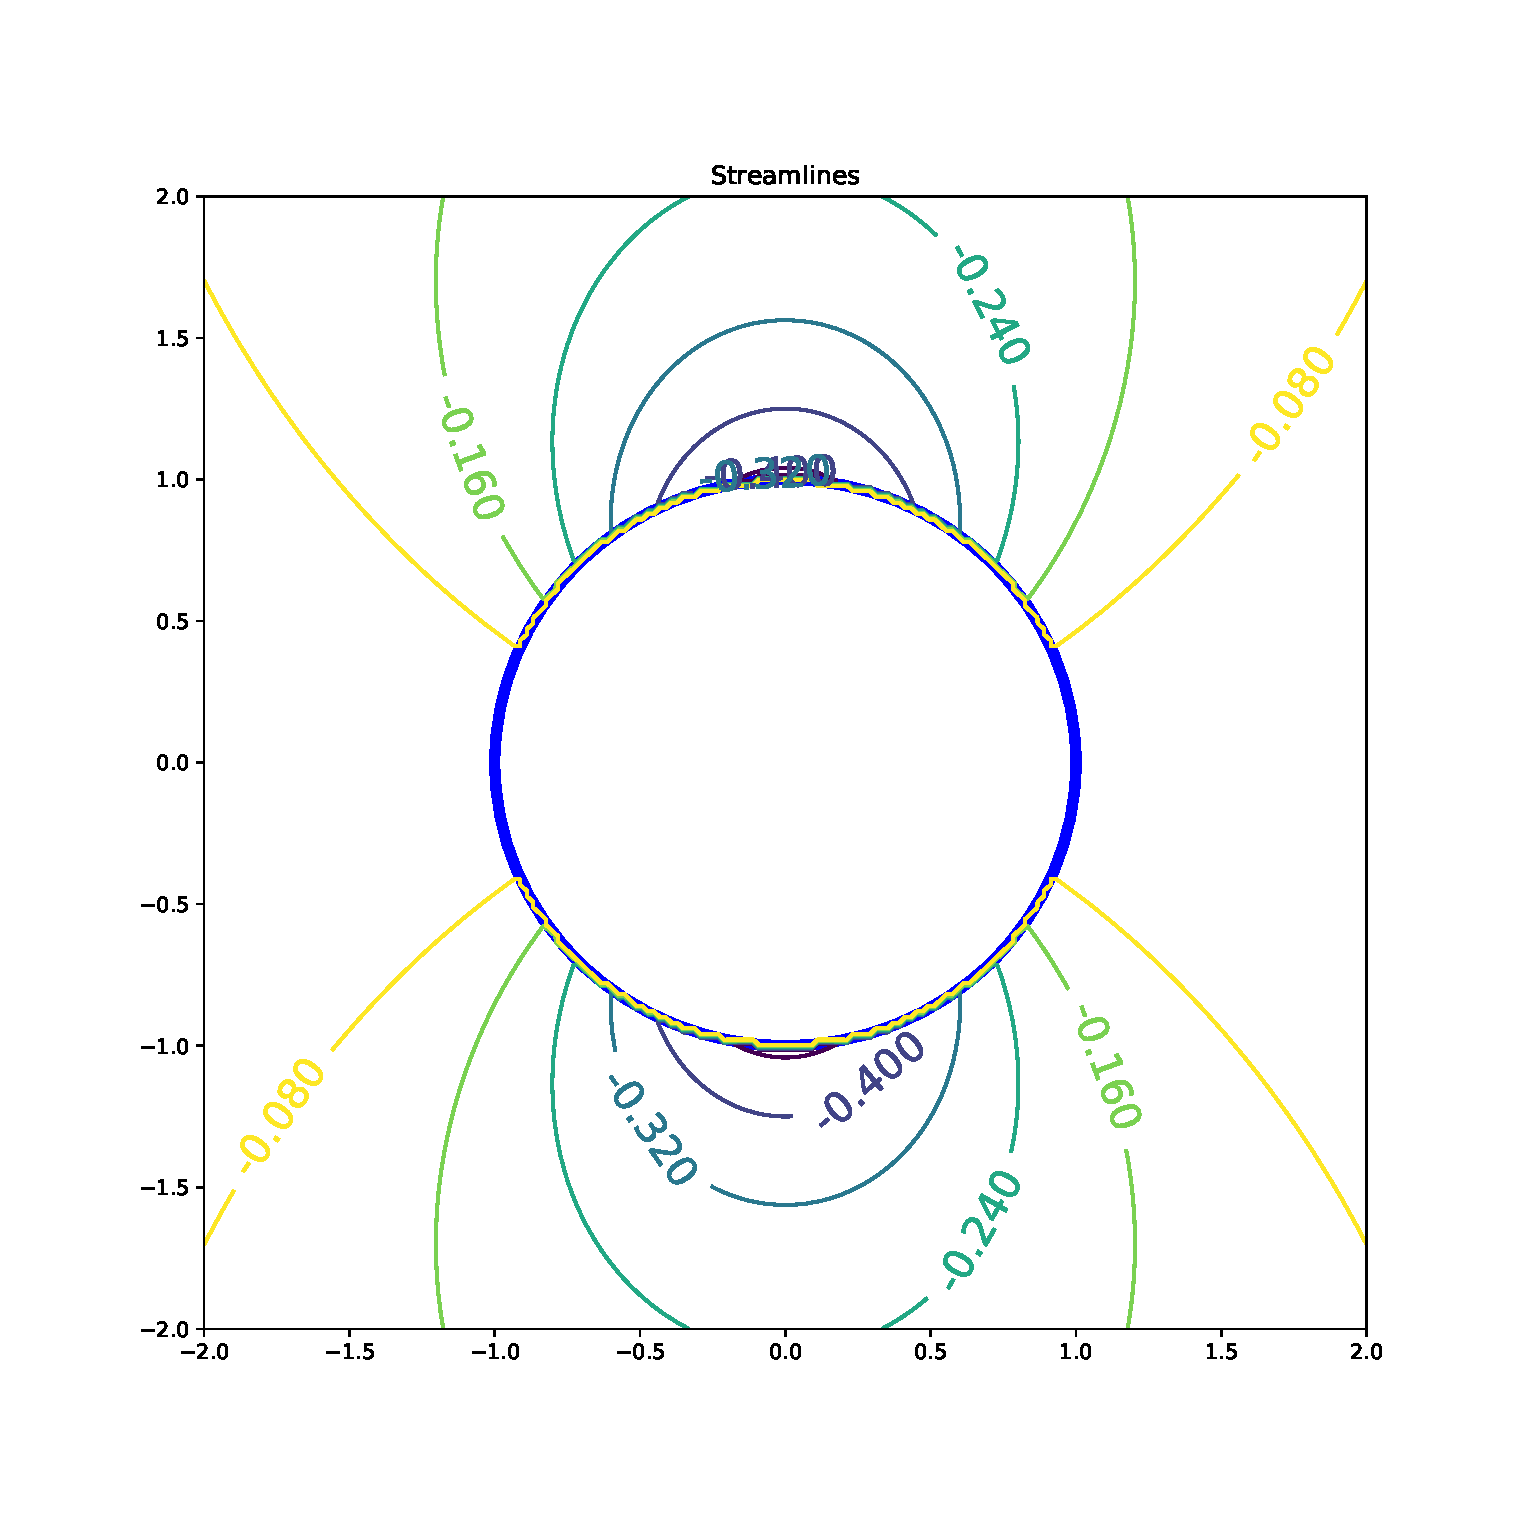
\includegraphics[width=0.4\linewidth]{figures/potential_flow_past_sphere_moving}
  \caption{\label{fig:potential_streamlines_moving_sphere}}
\end{figure}


\subsection{Exercises}

\begin{itemize}
\item \label{ex:u_from_psi_cylinder} Derive the velocity field for
  potential flow around a cylinder from $\psi$, solving Laplace's
  equation, plus the appropriate boundary conditions.

\item \label{ex:u_from_psi_sphere} Derive the velocity field for
  potential flow around a sphere from $\psi$, solving Laplace's
  equation, plus the appropriate boundary conditions. Notice that
  Laplace equation $\nabla^2 \bfA = 0$ may be written for $\psi$ using
  this identity:
  \begin{equation}
    \label{eq:psi_eq_from_A}
    \nabla^2 \left(  \frac{\psi(r,\theta)}{r \sin\theta } \bhe_\phi \right) =
    \frac{1}{r \sin\theta } 
    \left(
      \frac{\partial^2  }{\partial r^2} +
      \frac{1}{r^2} \left[
        \frac{\partial^2 }{\partial \theta^2} - 
        \cot(\theta) \frac{\partial }{\partial \theta}
      \right]
    \right) \psi \bhe_\phi .
  \end{equation}

\item Prove the previous identity. Notice that $\bfA$ is a vector
  field, so one need to apply the expression for the vector Laplacian
  of e.g. \cite{wiki:del}. The expressions are not so bad since the
  field is azimuthal only, and dependent on the other two components:
  $ \bfA = A(r,\theta) \bhe_\phi$.






\end{itemize}


%FOR POTENTIAL.TEX:




In axisymmetric flow,
\[
  \divu =
  {1 \over r^2}{\partial \left( r^2 u_r \right) \over  \partial r} +
  {1 \over r\sin\theta}{\partial \over \partial  \theta} \left( u_\theta\sin\theta \right) ,
\]
but an equivalent expression is
\[
  \divu =
  {\partial \left( r^2 u_r \sin\theta \right) \over  \partial r} +
  {\partial \left( r u_\theta\sin\theta \right)  \over \partial  \theta}
\]

so continuity is trivially satisfied with the choice
\ref{eq:u_from_psi_spherical}.


From the curl in spherical coordinates,
\begin{align}
  u_r     &= \frac {1}{r\sin \theta }
            \frac{ \left( \partial A  \sin \theta \right) }{\partial \theta }  \\
  u_\theta &= -\frac1{r} \frac{\partial (rA) }{\partial r} 
\end{align}
and we find
\begin{equation}
%  \label{eq:u_from_psi_spherical}
  \begin{split}
    u_r     &=  \frac1{r^2 \sin\theta} \frac{\partial \psi}{\partial \theta} \\
    u_\theta &= -\frac1{r   \sin\theta} \frac{\partial \psi}{\partial r}
  \end{split}
\end{equation}



Notice $A=\psi / \rho $ also in spherical coordinates !


\chapter{Gravity waves}

\begin{quote}
[Water waves] that are easily seen by everyone and which are usually
used as an example of waves in elementary courses [...] are the worst
possible example [...]; they have all the complications that waves can
have. \hfill (Richard Feynman, \textit{The Feynman Lectures on Physics})
\end{quote}

\section{Gravity waves}

Large waves, like those at the ocean, are driven by gravity. An
initial perturbation on the water surface, like an elevation, will
cause a rise in gravitational potenntial. As this energy is
transferred to kinetic energy, the water around it moves. Similarly to
a pendulum, an area below the mean surface will develop, which will be
filled with surrounding liquid. Thus, the perturbation travels away
from the initial disturbance.

The mathematical treatment of this problem is, in general, very
involved. This is mostly due to the presence of a free surface: the
water-air interface. Mathematically, its location is described by a
height function $\eta$:
\[
z=\eta  \qquad  \eta=\eta(x,y,t) 
\]
(if no overhangs are present). The fluid velocity is to be solved for
a domain between this surface at the ocean bottom, which is supposed
to be flat and at a height $z=-h$ (thus, $z=0$ is taken to be the
surface when no waves occur.)

We have the following boundary conditions for the velocity:
\begin{align}
%  p&=0 \\
  u_z(z=-h) &= 0 \\
  u_z(z=0) &=  \frac{\partial \eta}{\partial t}
\end{align}


The first one is the usual condition at a solid wall, and the last one
is called the ``kinematic condition'', expressing the fact that if the
surface moves up or down, the fluid must do the same in order to be
``stuck to it''.

We will assume an incompressible, irrotational fluid. The fist
assumption is a very reasonable one, and the second one turns out to
be not so bad, since for small waves there is little vorticity
creation (it mainly occurs at the bottom and on breaking waves).  The
assumption of negligible viscosity is likewise not so bad in this
case.



Let us assume a wave train that only depends on the $x$ component
(i.e. waves are very long in the $y$ direction):
\[
\eta = a \cos(kx -\omega t) .
\]
The amplitude $a$, is taken to be small (in the sense $a\ll \lambda$,
and $a\ll h$).

Given the assumptions above, the flow may be treated as a potential
flow, and moreover the only relevant coordinates will be $x$ and
$z$. However, the fields will be time-dependent in this problem,
e.g. $\phi=\phi(x,z,t)$.


The kinematic condition  implies
\[
\left. \frac{\partial \phi}{\partial z}\right|_{z=\eta} =
\frac{\partial \eta}{\partial t} .
\]
This is still a difficult expression, so we will approximate it by
\[
\left. \frac{\partial \phi}{\partial z}\right|_{z=0} =
\frac{\partial \eta}{\partial t} .
\]
(The difference between the two spactial derivatives may be quatified
by a Fourier expansion, in which the neglected terms are seen to be
higher order in $a$).

Let us consider the ansatz
\[
\phi = g(z) \sin(kx -\omega t ) .
\]
The kinematic condition then translates into $g'(0)=a\omega$.

The bottom condition clearly means
\[
\left. \frac{\partial \phi}{\partial z}\right|_{z= -h } = g'(-h)= 0 .
\]


All together, we are looking for a function with these boundary
conditions:
\begin{align}
  g'(0) &=  a \omega \\
  g'(-h) &= 0 .
\end{align}

However, the fact that Laplace equation must be satisfied places a
strong condition on the kind of function $g(z)$ may be:
\[
\nabla^2 \phi = 0 \qquad \to \qquad
g''(z)  \sin(kx -\omega t ) - g(z)  k^2 \sin(kx -\omega t ) = 0 ,
\]
which meanse
\[
g''(z)  = k^2 g(z) .
\]
Therefore, $g(z)$ must be an exponential function, with the decay
constant being exactly equal to $k$, the wave number. In general, the
solution is a linear combination of two exponentials. Instead of that,
we may write another less conventional expression using hyperbolic
functions. This is equivalent, since these functions are themselves
linear combinaions of exponentials. Moreover, we choose to center them
at $x=-h$ :
\[
g(z)  = a_1 \cosh(k(z+h)) + a_2 \sinh(k(z+h)) .
\]
By inspection, we realize $a_2=0$, since the $\sinh(k(z+h))$ function
was the ``wrong'' behavior at $z=-h$: it has a slope, while the
boundary condition implies it should not.

The kinetic boundary condition implies
\[
a_1 = \frac{a \omega}{ k \sinh(hk)  } .
\]
This is indeed the only value for which $g'(0)= a \omega $. The
potential is then
\[
\phi = \frac{a \omega  \cosh(k(z+h)) }{ k \sinh(hk)  }  \sin(kx -\omega t ) .
\]

From it, the velocity components may be found. These will have a term
featuring $\sin(kx -\omega t )$, a common expression for a traveling
wave. However, the theory is still incomplete since $\omega$ and $k$
are not unrelated in a physical wave, but coupled by the phase
velocity $c=\omega / k$. Remember how in sound waves this velocity was
related to fluid compressibility (to be precise, the square root of
the variation of pressure with density). In this case, such
relationship is as yet missing. Also notice that gravity has played no
role whatsoever, despite claims at the beginning of this chapter about
this factor being the driving force behind this process.

In order to find the missing link, let us remember our previous
expression for the Bernoulli principle, Eq.~\ref{eq:Bern_unsteady},
which can be written as
\[
\frac{\partial \bfu}{\partial t} +
\nabla \cdot \left[
  \frac12 u^2 + \frac{p}{\rho} + \varphi
  \right] =  \frac{p}{\rho}\nabla \cdot \bfu .
\]

In our case the fluid is incompressible, so the right hand side
vanishes. Also, in potential flow we may write the whole equation
compactly:
\[
\nabla \cdot \left[
  \frac{\partial \phi}{\partial t} +
  \frac12 u^2 + \frac{p}{\rho} + \varphi
  \right] =  0 .
\]

This means the whole term on which the divergence operator acts
must be constant in space, but not in time in general:
\[
  \frac{\partial \phi}{\partial t} +
  \frac12 u^2 + \frac{p}{\rho} + \varphi =  f(t) .
\]
This is the less-known unsteady Bernoulli principle.

In this particular case, since boundary conditions do not change in
time (in fact, they do, but we are taking the surface to be close to
$z=0$), any function $f(t)$ may be incorporated into the potential
by making the following trick:
\[
\phi' = \phi + \int_{t_0}^t f(t') dt' ,
\]
hence we may just take $f(t)=0$ in this particular problem.

If we examine the ``head'' term, $ \partial \phi / \partial t +
\frac12 u^2 + \frac{p}{\rho} + \varphi$ at the surface, we notice that
the pressure should be constant (equal to atmospheric pressure, as in
hydrostatics). The $u^2$ may be neglected within our
assumptions. Last, but not least, gravity finally appears in the
potential, $\varphi = g \eta $. This leaves us with
\[
\left.\frac{\partial \phi}{\partial t}\right|_{z=0} + g \eta = 0 ,
\]
often called the ``dynamic condition''. 

With our previous result, this means:
\[
\phi =  - \frac{a \omega^2  \cosh(k(z+h)) }{ k \sinh(hk)  }  \cos(kx -\omega t ) +
g a \cos(kx -\omega t ) =0 .
\]

The result is the following dispersion relation:
\[
\omega^2= g k \tanh(k h)
\]

This is a surprising result, despite being obviously dimensionally
correct, whith the two lengths in the problem, $\lambda=2\pi/k$ and $h$
providing the relevant lenght scales.

We may distinguish two limits.

\subsection{Shallow water}
If the bottom is small, compared to the wavelength $\lambda$, then
$kh = 2\pi h / \lambda $ is a small number, and we may approximate
$\tanh(kh)\approx kh$. Then,
\[
\omega^2= g h  k^2 \qquad \to \qquad \omega= k \sqrt{g h} .
\]

In this limit, the phase velocity is independent of velocity, which
means the process is non-dispersive:
\[
c =  \frac{\omega}{k} = \sqrt{ g h }  .
\]
The group velocity is of course equal to the phase velocity:
\[
c_\mathrm{g} =\frac{d\omega}{dk} = \sqrt{ g h } = c.
\]

The relevant length in this limit is the depth $h$, which provides the
correct dimensions to get a velocity.

Notice ``shallow'' is defined in relation to the wavelength. A seismic
wave may be excited at the deep sea by a geological process that may
involve tenths or hundreds of kilometers, much larger than the usual
sea depth, which is some few kilometers (its mean value is about
$\SI{3.8}{\kilo\meter}$.) The sea is then ``shallow'', and the speed
at which the perturbation travels will be about
\[
c \approx \sqrt{\SI{9.8}{\meter\per\second\squared} \times
  (\SI{4e3}{\meter}) } \approx \SI{200}{\meter\per\second}
  \approx \SI{700}{\kilo\meter\per\hour} 
\]
This is an astonishing speed, which is nevertheless in agreement with
measurements of these dramatic events.

\subsection{Deep water}

If the bottom is deep, compared to the wavelength $\lambda$, then $kh
= 2\pi h / \lambda $ is a large number, and its hyperbolic tangent is
very nearly $1$. In this limit,
\[
\omega^2 \approx g  k \qquad \to \qquad \omega= \sqrt{g k} .
\]
These waves are highly dispersive, since their phase velocity depends
on the wavelength:
\[
c =  \frac{\omega}{k} = \sqrt{ g /k  } =  \sqrt{ g \lambda / (2\pi)  }  .
\]

The group velocity is now different from the phase velocity. In fact,
it is one half that value:
\[
2 \log\omega = \log k + \log g \qquad \to \qquad
\frac{2}{\omega} \frac{d\omega}{dk} = \frac1{k} \qquad  \to \qquad
c_\mathrm{g} = \frac{c}{2}
\]

In deep waters, the only two length scales we may think of are the
wave amplitude $a$ and their wavength $\lambda$. As we expect the
amplitude to play no role (as long as it is small, $a\ll\lambda$), we
are left with the wavelength to provide the length scale.

Notice that waves high high wavelenghts travel faster. This explains
the groundsell phenomenon, by which waves generated by a far away
storm may arrive quickly at some shore. These waves may precede the
storm by a long time, if the storm does arrive at all. The velocity
grows larger and larger with the wavelength, but as we have seen in
the previous section, as the wavelength becomes comparable to the
depth there will be a crossover to some finite velocity.



\section{Gravity waves from energy}

There is an alternative derivation of the dispersion relation which is
interesting, and will be useful when the role of surface tension is
discussed in the next Section. \cite{whitham2011linear}

It begins by considering the energy of the whole system:
\[
  E := \int \left( T + U \right) d\bfr ,
\]
where the integral extends to the whole volume of the fluid, $T$ is
the total kinetic energy, and $U$ the potential energy:
\begin{align}
  T &= \frac12 \int ( \rho u^2 ) d\bfr \\
  U &=  \int (\rho \varphi) d\bfr 
\end{align}

For the simple case of gravity, the latter is simply given by
\begin{equation}
  U =    \int ( \rho g z ) d\bfr .
\end{equation}


If the flow is potential, the kinetic energy can be written as
\begin{equation}
  T = \frac12 \rho \int \left| \nabla\phi \right|^2 d\bfr ,
\end{equation}
a form that is appreciated in physics, where these sort of square
gradient theories are widely studied. (They are often called
``London-Linzburg-Landau'' theories, or a subset of those names, but
they begun, it seems, with van der Waals' seminal theory for the
liquid-vapor interface.)

In order to add more content ot our previous results, let us here
consider both an upper phase (``air'') of density $\rho'$ and a lower
one (``water'') with density $\rho$ (all primed variables refer to the
upper phase in this section). They are separated by the interfacial
surface at $z=\eta(x,y)$, but we will suppose that the surface
fluctuates around a well-defined position, which we will take, for
convenience, as $z=0$. The total potential energy is then
\[
U=
\iint dx dy   \int_{-H}^\eta  dz  ( \rho g z)
\iint dx dy   \int_\eta^{H'}  dz  ( \rho' g z)  ,
\]
where we suppose the bottom is at $z=-H$ and the air ends at $z=H'$. These
limits are not important, since we will consider later the limit
in which both are very large.

We may split the two integrals at $z=0$, the equilibrium surface:
\begin{align*}
  \iint dx dy   \int_{-H}^\eta  dz   &= 
                                       \iint dx dy   \int_{-H}^0  dz   +
                                       \iint dx dy   \int_{0}^\eta  dz   \\
  \iint dx dy   \int_\eta^{H'}  dz    &=
                                        \iint dx dy   \int_\eta^{0}  dz 
                                        \iint dx dy   \int_0^{H'}  dz  
\end{align*}

But, since two of those four integrals have fixed integration limits,
they will contribute a constant energy, so we may ignore them and just
write
\begin{align*}
  U &=\iint dx dy   \int_{0}^\eta  \rho g z  dz   -
  \iint dx dy   \int_\eta^{0} \rho' g z dz = \\
  & g  (\rho-\rho')  \iint dx dy   \int_0^{\eta} z  dz =
  \frac 12 g  (\rho-\rho')  \iint dx dy \eta^2 .
\end{align*}

It is natural that the potential energy is due to fluctiations of the
surface. However, the kinetic energy, which involves the motion of the
upper and lower fluid masses, can also be cast as a surface integral.
We may use the divergence (Gauss') theorem for this purpose. In order
to express the kinetic energy integrand as a divergence, we may write
\[
  \nabla\cdot [ \phi (\nabla \phi) ]  =
  |\nabla \phi|^2 +
  \phi \nabla^2 \phi .
\]
But the last term is null due to incompressibility. The same applies
to $\phi'$. This means the kinetic energy of the denser fluid can be
written as
\[
  T_1 = \frac12 \rho \int \nabla\cdot [ \phi (\nabla \phi) ] d\bfr \approx
  \frac12 \iint dx dy \phi (\nabla \phi) \bfe_z
\]
In this expression, we have applied Gauss theorem, and approximated
the true normal to the surface with its equilibrium value $\bhe_z$.
In other words,
\[
  T_1 = \rho 
  \frac12 \iint dx dy   \phi \frac{\partial \phi}{\partial z} 
\]
Adding the upper fluid, the total kinetic energy is
\[
  T = 
  \frac12 \iint dx dy
  \left(
    \rho \phi \frac{\partial \phi }{\partial z}
    -
    \rho'\phi'\frac{\partial \phi'}{\partial z}
  \right) ,
\]
because the outward-pointing normal of the upper phase is
approximated by $-\bhe_z$.
The appearance of those partial derivatives in the vertical direction
is appealing, because they are to be made equal to the vertical
velocity of the surface, according to boundary condition
\ref{eq:waves_bc2}.
%
Assuming a planar wave as in \ref{eq:wave_on_x}, and with our solution
for the potential in \ref{eq:wave_potential}, the necessary ingredients
are readily found:
\begin{align*}
  \frac{\partial \phi }{\partial z} &= \frac{\partial \eta }{\partial t}=
                                      a \omega \sin(kx -\omega t)  \\
  \phi(0) &= \frac{a \omega  }{ k }  \tanh(kh) \sin(kx -\omega t ) .
\end{align*}
For the upper phase, the appropriate potential is easily seen to be
\[
  \phi' = - \frac{a \omega  \cosh(k( h' - z )) }{ k \sinh( kh' )  } \sin(kx -\omega t ) ,
\]
since it must decay in the $z$ direction, satisfy the boundary
condition at $z=h'$, and the kinematic condition at the interface.

From now on, we will take the deep-water limit, leaving the general
case as an exercise to the reader. In this limit, the potentials approach
\[
  \phi(0)  = - \phi'(0) \to \frac{a \omega  }{ k }   \sin(kx -\omega t ) ,
\]
and the kinetic energy is
\[
  T = 
  \frac12 (\rho+\rho')     \frac{ (a \omega)^2  }{ k }
  \iint dx dy   \sin^2(kx -\omega t ) .
\]

For the same planar wave, the potential energy is
\[
  U = 
  \frac12 g (\rho-\rho') a^2  
  \iint dx dy   \cos^2(kx -\omega t ) .
\]

Now, the integral may be carried out: the $y$ integration yields
$L_y$, the length of the system in that direction, and on $x$ we may
have $N = L_x /\lambda $ total repetitions of the same wave, each one
of them we can integrate:
\begin{align*}
&  \iint dx dy   \cos^2(kx -\omega t ) =   \iint dx dy   \sin^2(kx -\omega t ) = \\
&  L_y N  \iint_0^\lambda dx   \cos^2(kx -\omega t ) =
  \frac12 L_y N \lambda = \frac12 A,
\end{align*}
where $A=L_x L_y$ is the total interfacial area.

This means both energies per surface area are
\[
  \frac{U}{A} = \frac14 g (\rho-\rho') a^2 \qquad
  \frac{T}{A} = \frac14 (\rho+\rho') \frac{ (a \omega)^2  }{ k } .
\]

The dispersion relation \ref{eq:water_disp_deep} is recovered (for
$\rho'=0$) if both energies are made equal. This is a tipical
requirement for oscillatory motion in physics, often called
``equipartition'' (not to be confused with a similar concept
in statistical mechanics). Its most well-known instance is the
harmonic oscillator.

A more formal justification comes from the Lagrangian%
\index{Lagrangian}.  This quantity (not to be confused with the
Lagrangian framework, or the Lagrangian derivative) is defined as
\[
  L = T - E .
\]

In classical mechanics, extremization of this quantity results in
the proper equations of motion. In our case,
\[
  \frac{L}{A} = \frac14 a^2
  \left(
    (\rho+\rho') \frac{ \omega^2  }{ k } -
    g (\rho-\rho')
  \right) .
\]

Extremization means that the partial derivatives of the Lagrangian
with respect to the parameters must be zero (technically, the
Lagrangian is not at a minimum or maximum, but at a saddle point).  In
our case, the only parameter is the amplitude, $a$, so
\[
\frac{\partial L}{\partial a} \implies 
    (\rho+\rho') \frac{ \omega^2  }{ k } -
    g (\rho-\rho') .
\]
This also implies $T=U$.

Hence, our previous deep-water dispersion relation
\ref{eq:water_disp_deep} is now modified to
\[
\omega^2  =    g  k \frac{\rho-\rho'}{\rho + \rho'}
\]

The combination $(\rho-\rho')/(\rho + \rho')$ is called the Atwood
number, and is closely $1$ when the denser fluid is much heavier than
the lighter one.


\section{Capillary waves}

The previous method can readilly accomodate capillary
waves\index{capillary waves}, also known as
``ripples''\index{ripples}. These are small waves that are dominated
by surface tension, not gravity. This is the dominant force at small
scales, and we will get an exact expression for the crossover lenght
below which this holds. Again, only the deep-water limit will be
considered.. Notice that, while this limit was bound to be violated
sooner or later for long gravity waves (when their wave-length begins
to be comparable to the water depth), capillary waves will eventually
comply with this limit at small wave-lengths.


The surface tension causes a cost in modifying an interface from its
equilibrium value:
\[
U_\mathrm{st} = \sigma (A - A_0),
\]
where $\sigma$ is the surface tension, with units of energy per area.

The area of a distorted surface in the Monge representation is given by
\[
  A = \iint dx dy \sqrt{
    1 +
    \left( \frac{\partial \eta}{\partial x} \right)^2 +
    \left( \frac{\partial \eta}{\partial y} \right)^2
  } .
\]
When fluctuation are not great, the cumbersome square root may
be expanded in Fourier series, and we find:

\begin{align*}
  A & \approx \iint dx dy 
  \left(
    1 + \frac12 \left[
      \left( \frac{\partial \eta}{\partial x} \right)^2 +
      \left( \frac{\partial \eta}{\partial y} \right)^2
    \right]
      \right) = \\
  &= A_0 + \frac12
  \iint dx dy 
  \left(
      \left( \frac{\partial \eta}{\partial x} \right)^2 +
      \left( \frac{\partial \eta}{\partial y} \right)^2
    \right)  
\end{align*}

For our perturbation \ref{eq:wave_on_x} we have,
\[
U_\mathrm{st} = \frac12   \sigma  
  \iint dx dy 
  \left( \frac{\partial \eta}{\partial x} \right)^2  =
  \frac14 \sigma A (a k)^2 ,
\]
where we have performed the same integration as in the
previous section.

Our Lagrangian is now
\[
  \frac{L}{A} = \frac14 a^2
  \left(
    \sigma  k^2 + 
    (\rho+\rho') \frac{ \omega^2  }{ k } -
    g (\rho-\rho')
  \right) .
\]

Its extreme now yields this dispersion relation:
\[
  \omega^2  =    g  k \frac{\rho-\rho'}{\rho + \rho'} +
  \frac{\sigma}{\rho+\rho'} k^3 .
\]
So we see that the short wave-length regime (high values of $k$) is
indeed dominated by a new $k^3$ term due to surface tension. The long
wave-length regime (low $k$ values) is, on the other hand, unaffected.

In order to analyze this expression, let us introduce reduced units
once more,
\[
\omega=\omega_0 \omega^* \qquad k = k_0 k^* ,
\]
where the typical angular frequency and wave vector are found by
demanding this simple expression holds:
\[
\omega^{*2}= k^* + k^{*3} .
\]

After some algebra, we find
\begin{align}
  \label{eq:capillary_k0}
  k_0&=\sqrt{\frac{ g (\rho-\rho') }{ \sigma }} \\
  \label{eq:capillary_om0}
  \omega_0^2 = g  \frac{ \rho-\rho' }{ \rho + \rho' } k_0
\end{align}


Now, the reduced phase velocity is given by
\[
  c^* := \frac{\omega^*}{k^*} =
  \sqrt{\frac{1}{k^*} +  k^* } ,
\]
so that it goes from a $\sim 1/\sqrt{k} $ growth at small $k$ (this is
the gravity regime) to a $\sim \sqrt{k} $ growth at high $k$ (surface
tension regime). It therefore has a minimum at some crossover
wave-vector $k_\mathrm{cross}$, which we may find by
\[
\frac{\partial c^* }{\partial k^*} = 0 .
\]

It is actually easier to differenciate $c^{*2}$. The value is found at
$k^*_\mathrm{cross} = 1$, at which
\[
c^*_\mathrm{cross} = \sqrt{2} .
\]

The values of $k_\mathrm{cross} $ are given by bringing back the
dimension factors in \ref{eq:capillary_k0} and \ref{eq:capillary_om0}.
The velocity is given by the factor
\[
  c_0 = \frac{\omega_0}{k_0} =
  \frac{[\sigma g (\rho-\rho')]^{1/4}}{(\rho-\rho')^{1/2}} .
\]

For water and air in standard conditions,
$\sigma=\SI{70}{\milli\joule\per\meter\squared}$,
and we find
\[
  k_\mathrm{cross} = \SI{374}{\radian\per\meter} \implies
  \lambda_\mathrm{cross} = \frac{2\pi}{k_\mathrm{cross}}=
  \SI{1.7}{\centi\meter} ,
\]
and
\[
  c_\mathrm{cross} =  \SI{23}{\centi\meter\per\second} .
\]
This is the scale below wich surface tension is important, and the
phase velocity is the lower possible.

The group velocity is defined as
\[
  c_\mathrm{gr} := \frac{\partial \omega }{\partial k}  .
\]
Notice that, by differenciating $c = \omega / k$ with respect to $k$
it is easy to prove the identity:
\[
  c_\mathrm{gr} =  c + k \frac{\partial c }{\partial k}  .
\]
This clearly shows that the a difference in the values of the two
velocities is caused by dispersion: the phase velocity having a
dependence on the wave vector, as evident in the $dc/dk$ term. This
also shows that at the crossover velocity, where this term vanishes,
both velocities are the same. These waves are, then the only
non-dispersive ones possible in the deep-water regime.

The expression for the group velocity is, in reduced units,
\[
  c^*_\mathrm{gr} :=  \frac{1+ k ^2}{2\sqrt{k + k^3} } .
\]
It then goes from a low-$k$ regime in which $c_\mathrm{gr} \to c /2 $
(gravity) to a high-$k$ regime with $ c_\mathrm{gr} \to 3 c /2 $
(surface tension). In the latter regime, the group velocity is $50\%$
faster than the phase velocity.  In
\ref{fig:gravity_capillary_dispersion_k} we plot both velocities as
functions of the reduced wave-vector. Both are seen to cross at a
value of $1$.  In Figure \ref{fig:gravity_capillary_dispersion_lambda}
the same is plotted as a function of wave-length. The crossing takes
place at the reduced wave-length value of $\lambda^*=2\pi$.

\begin{figure}
  \centering
  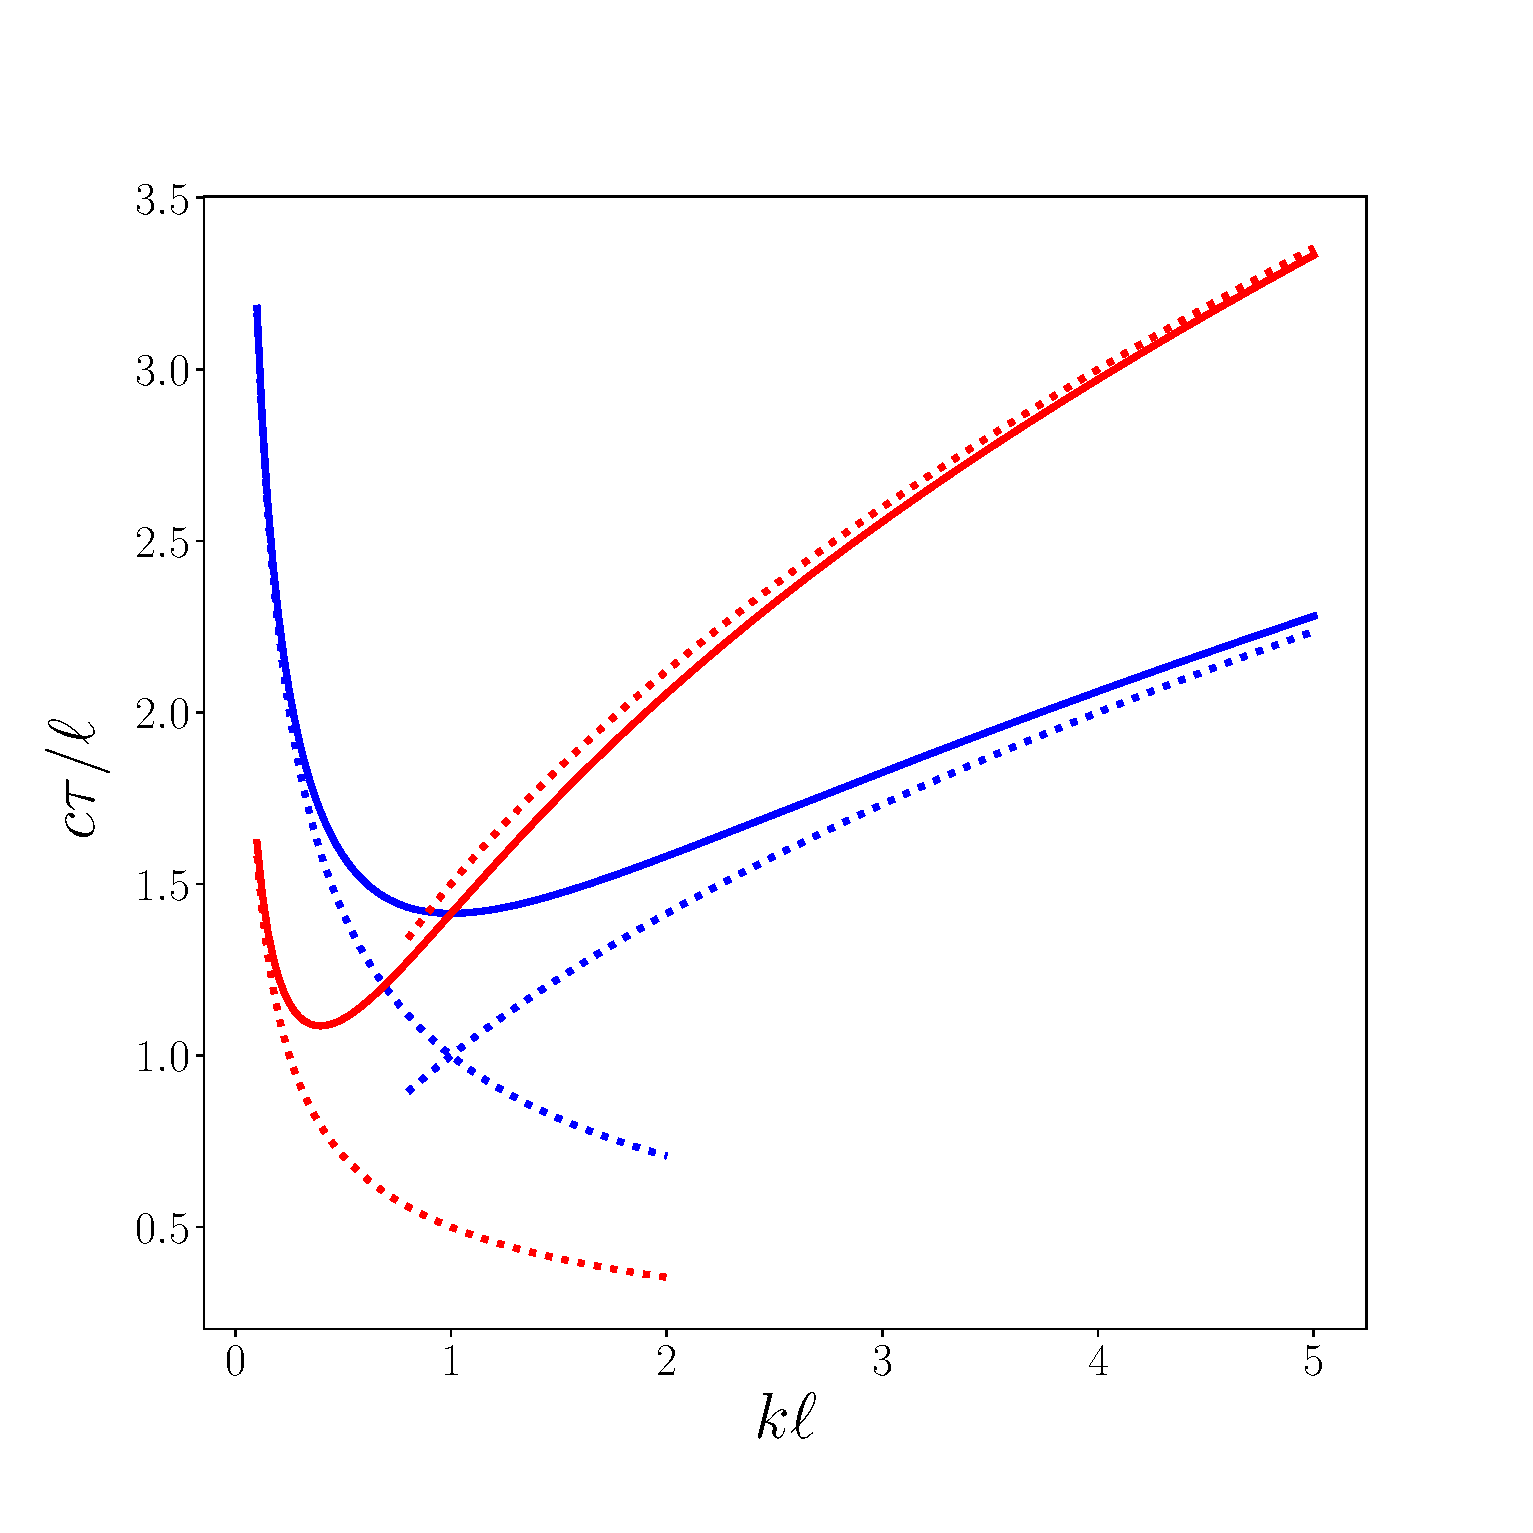
\includegraphics[width=0.4\linewidth]{figures/gravity_capillary_dispersion_k}
  \caption{\label{fig:gravity_capillary_dispersion_k}}
\end{figure}


\begin{figure}
  \centering
  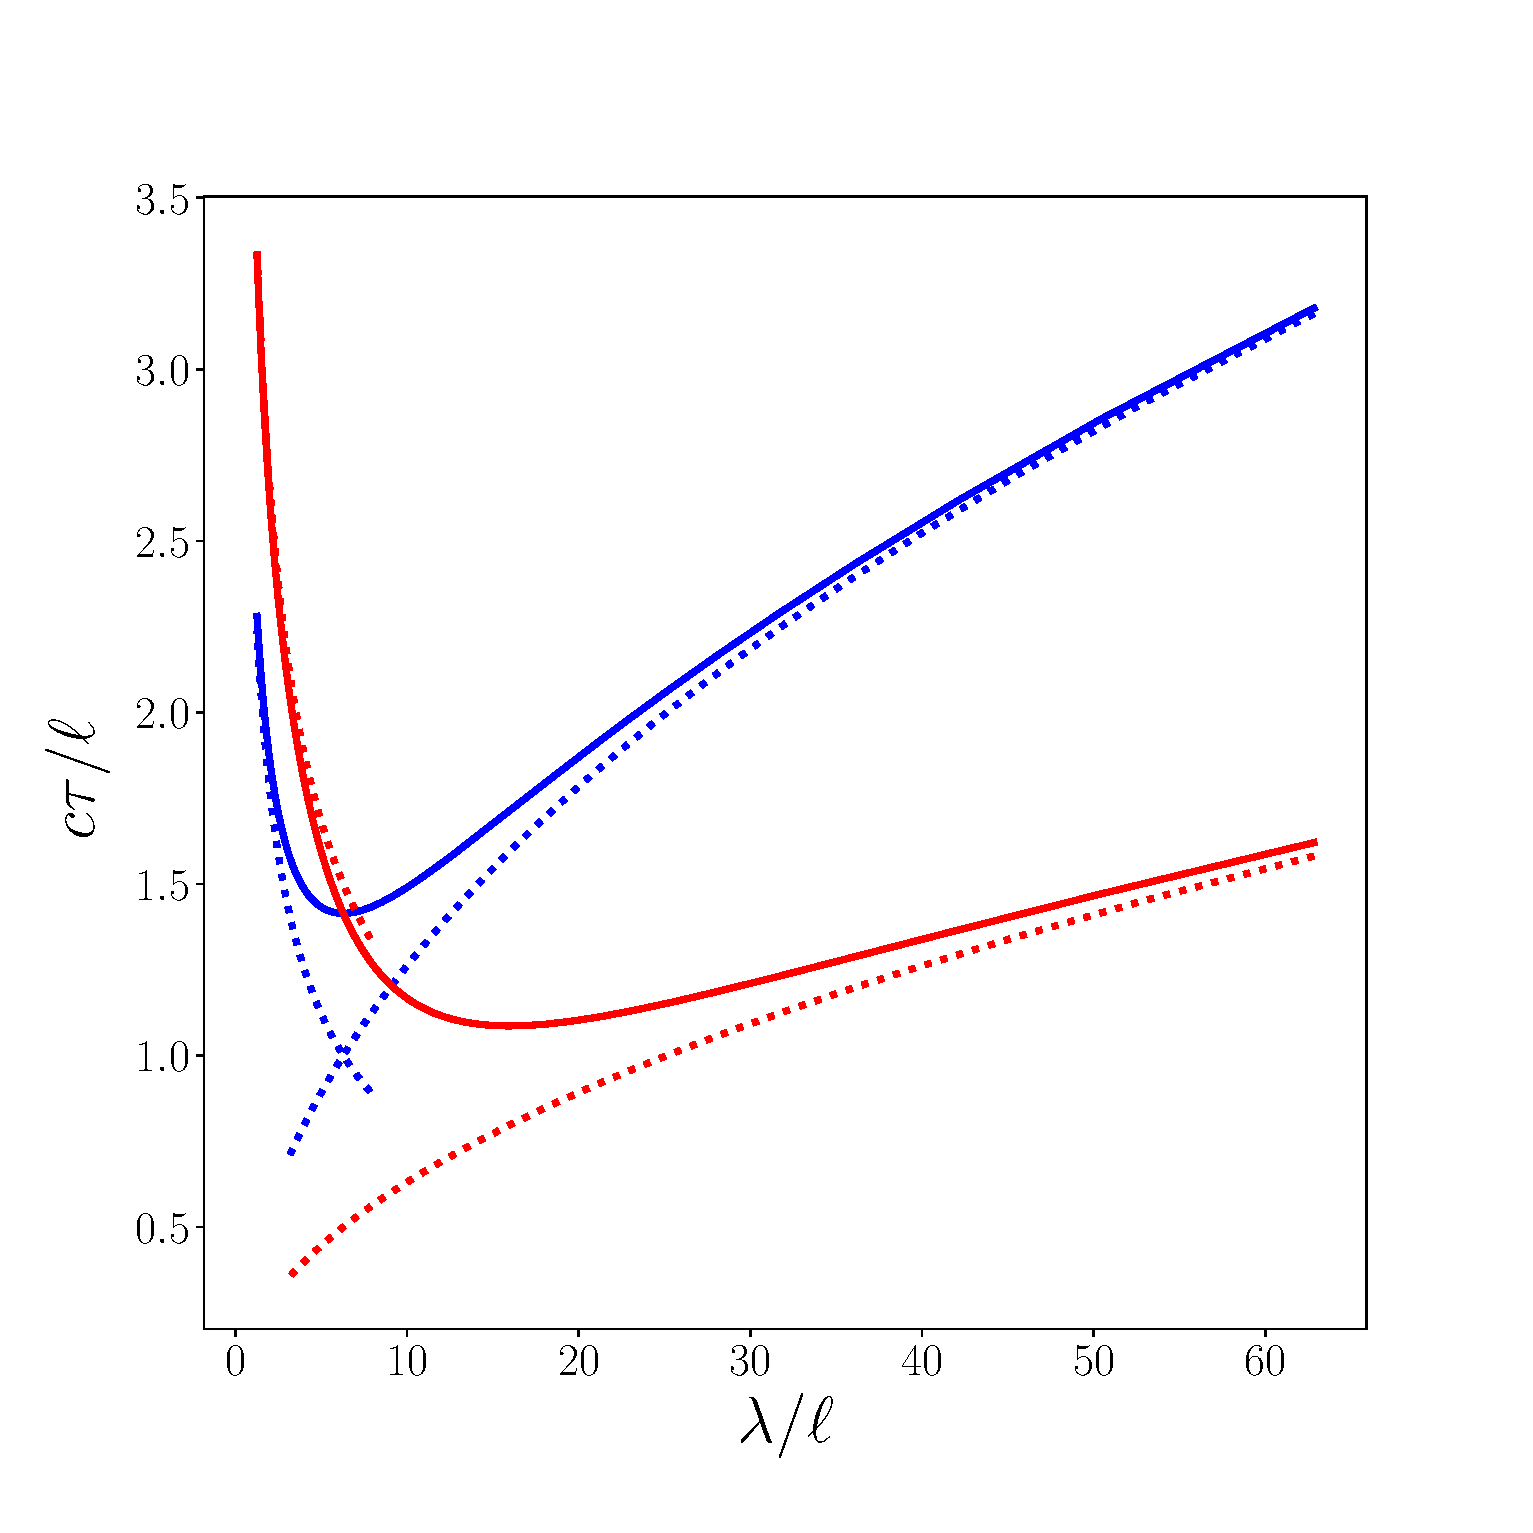
\includegraphics[width=0.4\linewidth]{figures/gravity_capillary_dispersion_lambda}
  \caption{\label{fig:gravity_capillary_dispersion_lambda}}
\end{figure}



\chapter{Work and energy}

Let us find the work done on a fluid particle.

The First Law of thermodynamics tells us this change is due
to work (no heat exchange is considered here):
\[
dE=dW
\]

On the $x$ direction, this work will be given by the distance
travelled by the left wall in the $x$ direction times the pressure
force:
\[
dW_x (\mathrm{left})  = u_x \Delta t p A .
\]

This is work done on the particle (if $u_x$ is positive), hence its
sign. There will be a similar contribution from the right wall, so the
total work given by the $x$ direction will be
\[
dW_x = u_x \Delta t p A  -  u_x'  \Delta t p' A .
\]
By expanding in a Taylor series, this may be written as
\[
dW_x = - \frac{\partial p u_x}{\partial x} \Delta x A \Delta t.
\]

Now, adding the other three components we find
\[
\frac{dW}{dt} = - V \nabla\cdot (p\bfu) .
\]

The right hand side may be expanded
\[
\nabla\cdot (p\bfu) =
 p \nabla\cdot \bfu + 
 \bfu \cdot \nabla p .
\]

Recalling that, from the Euler equation \ref{eq:Euler_momentum} ,
\[
\nabla p  = \rho \bfg - \rho \frac{d \bfu}{dt} ,
\]
we may write
\[
\frac{1}{V} \frac{dW}{dt} =
-  p \nabla\cdot \bfu +
\rho  \bfu \cdot \frac{d \bfu}{dt}  -
\rho  \bfg \cdot  \bfu .
\]

Now, multiplying by $1/\rho$:
\begin{equation}
  \label{eq:specific_energy}
  \frac{d \epsilon }{dt} =
  \bfu \cdot \frac{d \bfu}{dt}  -
  \bfg \cdot  \bfu 
  -  \frac{p}{\rho} \nabla\cdot \bfu ,
\end{equation}
where we have defined the specific energy $\epsilon=E/M$.

This may be written as
\[
\frac{d}{dt} \left[
  \epsilon - \frac12 u^2  + \bfg \cdot \bfr
  \right] = -  \frac{p}{\rho} \nabla\cdot \bfu ,
\]
or
\[
\frac{d}{dt} \left[
  \epsilon - \frac12 u^2  - \varphi
  \right] = -  \frac{p}{\rho} \nabla\cdot \bfu ,
\]
%
This is clearly a law for
\[
e = \epsilon - \frac12 u^2  - \varphi ,
\]
where we define $e$, the specific internal energy as the total energy
minus kinetic energy, minus gravitational potential energy. In other words,
\[
\epsilon  = e  + \frac12 u^2  + \varphi .
\]

The specific internal energy then satisfies a convection equation with
a source term due to the divergence of the velocity
\begin{equation}
  \label{eq:Euler_energy}
  \frac{d e}{dt}  = -  \frac{p}{\rho} \nabla\cdot \bfu ,  
\end{equation}

Notice also that in the steady state,
\[
\bfu \cdot \nabla e = -  \frac{p}{\rho} \nabla\cdot \bfu.
\]
But, recalling our steady Bernoulli principle,
Eq. \ref{eq:Bern_u_times}, replacing
$\frac{p}{\rho} \nabla\cdot \bfu$, we arrive at the steady state
Bernoulli equation for a compressible fluid:
\[
\bfu \cdot \nabla \left[ e + \frac12 u^2 + \frac{p}{\rho} + \varphi
  \right] = 0 ,
\]
%
which tells us the combination $ e + \frac12 u^2 + \frac{p}{\rho} +
\varphi = \epsilon + \frac{p}{\rho} $ is constant along streamlines.
Notice that, by the definition of enthalpy,
\[
H= E + P V ,
\]
the specific enthalpy is
\[
h=H/M = e + p / \rho ,
\]
so the Bernoulli principle claims that the total specific enthalpy
($h'=h + \frac12 u^2 + \varphi$) is constant along streamlines.

We may also find an equation for the enthalpy. In
Eq. \ref{eq:Euler_energy} above, the right hand side may be changed
using the continuity equation:
\[
- \rho \nabla\cdot \bfu = \frac{d\rho}{dt} .
\]
which means
\[
-  \frac{p}{\rho} \nabla\cdot \bfu =
\frac{p}{\rho^2} \frac{d\rho}{dt}
\]

But
\[
\frac{d (p / \rho) }{dt} =
\frac{ 1 }{\rho} 
\frac{d p }{dt} -
\frac{ p }{\rho^2} 
\frac{d \rho }{dt}  .
\]
Hence,
\[
\frac{d ( e + p / \rho) }{dt} = \frac{ 1 }{\rho} \frac{d p }{dt} ,
\]
or
\[
\frac{d h }{dt} = \frac{ 1 }{\rho} \frac{d p }{dt} .
\]
Changes in the enthalpy are therefore tied to changes in pressure.


\subsection{Heat flux}

In the case that some heat flux is present, the First Law of
thermodynamics reads:
\[
dE=dW + dQ .
\]

The influx of heat to the particle, $dQ$, will enter our equations
from a vector heat flux $\bfq$, with units of energy/(area $\times$
time). For example, the heat influx due to transfer in the $x$ direction
will be
\[
dQ_x= \bfq dt dy dz - \bfq(x+dx) dt dy dz \approx
      - V \, dt \, \frac{\partial\bfq}{\partial x},
\]
where in the last approximation a Taylor expansion has been employed,
as should be customary by now.

Altogether, the total heat flux rate is
\[
\frac{dQ}{dt} = -V \nabla\cdot \bfq,
\]
and the final equation for the rate of change of specific internal
energy of an ideal fluid is
\begin{equation}
  \label{eq:Euler_energy_w_q}
  \rho \frac{de}{dt}  = -  p \nabla\cdot \bfu  - \nabla\cdot \bfq .
\end{equation}


The heat flux must be either due to an external source, or due to heat
diffusion. In the latter case, a well-known theory is Fourier's law, by
which the flow is due to a temperature gradient:
\[
\bfq=- k \nabla T ,
\]
where $k$ is the heat diffusion coefficient. The temperature does not
appear in the energy equation, but a common assumption is that
\[
e = c T ,
\]
where $c$ is the specific heat, taken as constant. Then,
\[
\rho  c \frac{d T }{dt}  = - p \nabla\cdot \bfu  + k \nabla^2 T .
\]

For an incompressible fluid,
\[
 \frac{d T }{dt}  = \frac{ k }{ c \rho} \nabla^2 T  = \alpha \nabla^2 T ,
\]
where $\alpha = k / (c \rho)$, a constant if $\rho$ is. This is the
convective Fourier heat equation (it is not the most common Fourier
law, due to the derivative being convective, and not just partial.)



\part{Real fluids}


\chapter{Navier-Stokes equations}

Let us focus again on a fluid particle, as we did on \ref{sec:}, but
now focusing on how the particle itself distorts as a consequence of a
velocity field.

All possible distorsions of a particle will be a combination of the
following:
\begin{enumerate}
 \item Translation
 \item Rotation
 \item Shear
 \item Dilation
\end{enumerate}

A translation is just the motion of its center of mass from one place
to another, and for a small time is given simply by $\bfu dt$. The
other motions are more complicated, since they involve spatial
derivatives of the velocity. They must: for a constant velocity field
translation is the only mode that occurs.

\subsubsection{Rotation}

We will refer to particle in figure \ref{fig:}, with vertices A, B,
and C. Vertex D plays no role --- also, it is sufficient to focus on
the face that is portrait, even if the shape of a particle is supposed
to be a cube. It is straightfoward to include the other faces, as we
will see.

After a small time $d$ the particle has distorted, so that the
vertices are now at positions A', B', C', and D'.

\begin{figure}
  \centering
  
\includegraphics[width=0.4\linewidth]{figures/particle0}
  \caption{\label{fig:particle0}}
\end{figure}



Let us call $\alpha$ the angle between the $x$ axis and the A'-B'
edge, with the usual counter-clockwise convention as
positive. Similarly, $\beta$ is the angle between the A'-C' edge and
the $y$ axis, with the same convention. It is obvious that a net
rotation takes place if e.g. both angles are positive. If, on the
other hand, they are equal in magnitude but differ in sign, no
rotation takes place. This makes it reasonable to define the
rotation as the average of both angles:
\[
d\Omega_z = \frac12
\left(
        \alpha + \beta
\right) .
\]

Now, angle $\alpha$ will always be very small as $dt$ gets very
tiny. Hence, we may approximate it by its tangent:
\[
\alpha \approx \frac{d\ell}{dx'}
\]



\begin{figure}
  \centering
  
\includegraphics[width=0.4\linewidth]{figures/particle1}
  \caption{\label{fig:particle1}}
\end{figure}

For a small time, we have the following:
\[
dx'=x(B')-x(A') \approx
(dx+v_x(B) dt) - v_x(A) dt \approx
dx+
\left(
v_x(A) +
\frac{\partial v_x}{\partial x} dx
\right ) dt - v_x(A) dt = dx + \frac{\partial v_x}{\partial x} dx dt ,
\]
where we have taken the origin to coincide with the position of A. The
partial derivative is supposed to be evaluated at A, but in the limit
as $dx$ goes to zero it is just ``at the particle''. Similarly, the opposing
side is:
\[ 
d\ell = y(B')-y(B) \approx
v_y(B) dt \approx
\left(
v_y(A) +
\frac{\partial v_y}{\partial x} dx
\right ) dt = \frac{\partial v_y}{\partial x} dx dt ,
\].

Therefore, to first order in $dt$:
\[
\alpha \approx \frac{\partial v_y}{\partial x}  dt .
\]
In other words, the rate of change of the angle is
\[
\frac{d \alpha}{dt} = \frac{\partial v_y}{\partial x}  .
\]
Notice the cross derivative: what is relevant is the change of the
vertical component of the velocity with the horizontal coordinate.

A similar calculation for the other angle reveals
\[
\frac{d \beta}{dt} = - \frac{\partial v_x}{\partial y}  .
\]

Taking all
\[
\frac{d\Omega_z}{dt} = \frac12
\left(
  \frac{\partial v_y}{\partial x}  -
  \frac{\partial v_x}{\partial y}
\right) .
\]

This may sound familiar to the reader, since the curl in Cartesian
coordinates has a $z$ component with exactly the same expression, but
the factor of $1/2$. This analysis may be carried out for
rotations about the other two Cartesian axes, with the end result that
\[
 \frac{d \bm{\Omega} }{dt} = \frac12 \vort .
\]

The curl is therefore twice the rate of rotation of a fluid particle.


An example

Let us consider a uniform circular motion about the origin:
\[
\bfr =
\begin{cases}
&x=r \cos(\omega_0 t) \\
&y=r \sin(\omega_0 t) .
\end{cases}
\]
The velocity field is
\[
\bfu =
\begin{cases}
&u_x= -r \omega_0 \sin(\omega_0 t) = -\omega_0 y \\
&u_y=  r \omega_0 \cos(\omega_0 t) =  \omega_0 x.
\end{cases}
\]

If we compute the curl of this field, its only component is the $z$ one:
\[
\omega_z= \left(
  \frac{\partial (\omega_0  x)}{\partial x}  -
  \frac{\partial (- \omega_0 y) }{\partial y}
\right) =  2 \omega_0 . 
\]

Therefore, the curl indeed is twice the angular velocity.


\subsubsection{Strain}




\section{Stress tensor}

Let us return again to our particle in order to analyze its movement
when stress forces are applied onto its walls. The pressure force may
be consider a special case of the latter, but stress forces may also
have a shear component.

Thus, the horizontal force will be given by, in part, by the
contributions due to the walls at the left, back, and bottom
\begin{equation}
  \label{eq:wall_shear_stress}
  \left. dF_x \right|_\text{l,bk,bm} =
  % - p         dy\, dz
    \tau_{xx} dy\, dz
    \tau_{yx} dx\, dz
    \tau_{zx} dx\, dy .
\end{equation}
%
The compression stress $\tau_{xx}$ is therefore quite similar to the
pressure (see (Eq \ref{eq:}), and in fact will be seen to include a
$-p$ term. The minus sign appears because normal stresses are
historically defined as positive if pointing outside the particle
(i.e. in the direction of the normal vector).
%
%where we include not only the pressure force, as before 
%and a compression stress $\tau_{xx}$ quite similar to it,
In addittion, two shear stress forces appear. One of them, $\tau_{yx}
dx\, dz$ is the horizontal shear force on the back wall ($dx\, dz$
actually equals $dx\, dy$, but it is clearer to write it this
way). Similarly, $\tau_{zx} dx\, dy $ is the horizontal stress force
at the bottom wall.

Notice the convention for labeling: $\tau_{ij}$ is the stress in the
$j$ direction on a face normal to axis $i$. I.e. the left face has the
same convention as the right one, the back as the front, the top as
the bottom.

%First, the normal stress is
%$\tau_{xx} \parallel \bfn $. From it,
%$\tau_{xy} \parallel \bfe_z\times \tau_{xx} $,
%$\tau_{xz} \parallel \tau_{xx} \times \bfe_y $, respecting the
%$(x,y,z)$ cyclic order. A quick way to realize this is by considering
%the top face, on which these three directions coincide with the
%Cartesian axes. The directions on other faces are found by rotating
%these directions accordingly. The right hand may be used for this
%purpose.

To get the whole horizontal force, the contributions from the other
three walls must be considered:
\[
\left. dF_x \right|_\text{r,ft,up} =
%- p         dy\, dz
  \tau_{xx}(x+dx,y   ,z   )  dy\, dz +
  \tau_{yx}(x   ,y+dy,z   )  dx\, dz +
  \tau_{zx}(x   ,y   ,z+dz)  dx\, dy .
\]
%This time, the sign convention is positive.

To get the total horizontal force due to stresses, the two contributions
must be substracted:
\[
dF_x =
\left( \tau_{xx}(x+dx,y   ,z   ) - \tau_{xx} \right) dy\, dz +
\left( \tau_{yx}(x+dx,y   ,z   ) - \tau_{yx} \right)  dx\, dz +
\left( \tau_{zx}(x+dx,y   ,z   ) - \tau_{zx} \right) dx\, dy .
\]
Notice that the substraction is in order: if the stresses are the same
on those faces, the resultant force will then be zero (those forces
may exert a net torque, but not a force).  In general, they will be
different on those faces, as as been made explitic on their arguments.

The choice is such that an variation in a given direction is assigned
a positive sign. This affects later results, in particular the fact
that the pressure appears with a negative sign.

Expanding in Taylor series, we get the following net horizontal force:
\[
 dF_x  =
%-\frac{\partial p      }{\partial x}  dx\, dy\, dz
% +
 \left(\frac{\partial\tau_{xx}}{\partial x}  dx\right)\, dy\, dz
+\left(\frac{\partial\tau_{yx}}{\partial y}  dy\right)\, dx\, dz
+\left(\frac{\partial\tau_{zx}}{\partial z}  dz\right)\, dx\, dy .
\]

The volumetric horizontal force is then,
\[
f_x  =
%-\frac{\partial p      }{\partial x}
 %+
 \frac{\partial\tau_{xx}}{\partial x}
+\frac{\partial\tau_{yx}}{\partial y}
+\frac{\partial\tau_{zx}}{\partial z} .
\]

With integer notation for Cartesian coordinates:
\[
 df_1  =
%-\frac{\partial p      }{\partial x_1}
 %+
 \sum_{j=1,2,3}
 \frac{\partial\tau_{j1}}{\partial x_j} .
\]


In general, for any component we will have:
\[
 df_i  =
%-\frac{\partial p      }{\partial x_i}
 %+
 \sum_{j=1,2,3}
  \frac{\partial\tau_{ji}}{\partial x_j} .
\]

In order to use vector notation, we have to introduce the
divergence of a tensor:
\[
\nabla \cdot \tau = \sum_{j=1,2,3}
  \frac{\partial}{\partial x_j}  \tau_{ji} ,
\]
 which results in a vector:
\[
 d\bff  =
%-\nabla p
 %+
 \nabla \cdot \tau .
\]
%
The tensor $\tau$ has components $\tau_{ij}$. There is also
the matrix notation, by which
\[
\nabla \cdot \tau = \nabla\tran  \tau ,
\]
where $\nabla\tran$ is a transposed (row) vector operator, multiplying
matrix $\tau$ from the left.

The resulting Navier-Stokes equation is then,
\[
\rho \frac{d\bfu }{dt} = \nabla \cdot \tau   + \rho \bfg .
\]



\subsection{Newtonian fluids}

The previous equation is still too general, and a connection between
stress and strain is still needed. Here we consider the case in which
there is a linear relationship between both, which involves the
coefficient of viscosity.

To begin with, let us consider a simple case in which a fluid is
confined between two planes. One of them moves sideways with a certain
speed $u_0$, while the other is kept fixed. After a certain transient,
some force is needed in order to keep this shearing. The simplest
expression is
\[
F= \mu A \frac{u_0}{L} .
\]
The force is proportional to the area and to the velocity difference
between the planes. It is also inversely proportional to their
separation, $L$ (this fact being the least obvious). Finally, a
constant of proportionality is given by $\mu$, the viscosity
coefficient, or simply ``the viscosity''. This constant may vary with
temperature, density, pressure, but the point with Newtonian fluids is
that it does not vary with the velocity field (or its
derivatives). Later, in section \ref{sec:}, this flow will be solved
as a solution of the Navier-Stokes equations, the Couette flow. There,
it will be shown that the velocity is everywhere in the direction of
the force exerted on the upper plane, let us call it $x$, and varies
linearly between the planes, in the $y$ direction. Therefore, the only
components of the strain rate tensor are $\epsilon_{xy} =
\epsilon_{yx} = u_0 / ( 2 L )$. We therefore have
\[
\tau_{xy} = \mu  \epsilon_{xy} .
\]

With these in mind, let us look for a general relationship between
$\tau$ and $\epsilon$. This is much easier if we go to the principal
strain axes. These are the coordinates on which the strain rate is
diagonal. Such coordinate system always exist, since the strain rate
tensor is symmetric. Notice that in these system strains are not due to
shear, only to dilations.

A simple example would be to consider the flow $u_x = u_0 y / L$
(again, Couette flow). In this case,
\[
\epsilon=
\begin{pmatrix}
  0           &   u_0/(2L)  \\
   u_0/(2L)   &   0
\end{pmatrix} .
\]

It is easy to find the two eigenvalues and associated eigenvectors of
this matrix:
\begin{align*}
  \lambda_1=  u_0/(2L) \qquad &\bfv_1=(1/\sqrt{2}) \begin{pmatrix} 1 &  1 \end{pmatrix}\tran \\
  \lambda_1= -u_0/(2L) \qquad &\bfv_2=(1/\sqrt{2})  \begin{pmatrix} 1 &  -1 \end{pmatrix}\tran \\
\end{align*}
Notice the first eigenvalue correnspond to a dilation along the $x=y$
diagonal, while the second is a compression along the $x=-y$ one.

The diagonal strain rate matrix is then:
\[
\tilde{\epsilon}=
\begin{pmatrix}
  u_0/(2L)   & 0 \\
  0          & - u_0/(2L)
\end{pmatrix} .
\]

It is crucial to realize that the stress tensor is also diagonal in
this coordinate system. Otherwise, a pure dilation in one of the
principal directions would cause a shear stress in some other
direction. This does not mean, however, that the two tensors are
simply proportional. Instead, we may posit, for the top-most element
\[
\tilde{\tau}_{xx}=
- p + 
C_1 \tilde{\epsilon}_{xx} +
C_2 \tilde{\epsilon}_{yy} +
C_3 \tilde{\epsilon}_{y} .
\]
We have added a $-p$ term that has to be there even when there is no
movement. This is needed, since a diagonal stress tensor $\tau=-p\eye$
produces the $-\nabla p$ term of hydrostatics (in Couette flow, $p$ is
constant, and this term is not needed.) The minus sign of $-p$ stems
from the fact that the pressure force points toward the interior of a
particle.

If isotropy is assumed, there should be no distinction between
traverse directions $y$ and $z$. Therefore, $C_2=C_3$, and
\[
\tilde{\tau}_{xx}=
- p + 
C_1 \tilde{\epsilon}_{xx} +
C_2 ( \tilde{\epsilon}_{yy} +  \tilde{\epsilon}_{y}  ) =
- p + 
K \tilde{\epsilon}_{xx} +
C_2 ( \tilde{\epsilon}_{xx} + \tilde{\epsilon}_{yy} +  \tilde{\epsilon}_{y}  ) ,
\]
where the constant $K=C_1-C_2$. Notice the $C_2$ term is the
divergence of the velocity. But, it is also the trace of the strain
tensor, a quantity which is invariant under change of basis. We can
now write:
\[
\tilde{\tau}_{xx}=
- p + C_2 \nabla\cdot \bfu 
K \tilde{\epsilon}_{xx} .
\]

There will be similar expressions for $\tilde{\tau}_{yy}$ and
$\tilde{\tau}_{zz}$, but in them the coefficients must be the same ---
otherwise isotropy will be violated. Taking all together,
\[
\tilde{\tau}=
K \tilde{\epsilon}
+ ( - p + C_2 \nabla\cdot \bfu ) \eye.
\]

Now, we may go back to the original Cartesian system and find
\[
\tau=
K \epsilon
+ ( - p + C_2 \nabla\cdot \bfu ) \eye.
\]
The stress tensor is then also symmetric, a fact that is required in
order the particle be torsion-free (remember the fact that rotations
have no stress associated.)

A comparison with our previous result reveals $K=2\mu$. The constant
$C_2$ is called, in the theory of elasticity ``the second Lam\'e
coefficient'', and receives the symbol $\lambda$ (it is also called
the ``second viscosity coefficient'', $\mu$ being the first.) Then,
\[
\tau=
2 \mu \epsilon + ( - p + \lambda \nabla\cdot \bfu ) \eye.
\]

To make this explicit, this means that diagonal terms have the form
\begin{equation}
  \label{eq:tau_diagonal}
  \tau_{ii}=
  2 \mu \epsilon_{ii}  - p + \lambda \nabla\cdot \bfu ,
\end{equation}
while off-diagonal terms are
\begin{equation}
  \label{eq:tau_off_diagonal}
  \tau_{ij}=  2 \mu \epsilon_{ij} \qquad j \ne i
\end{equation}


(Why not always work in the system of principal axes? The answer is
simple: principal axes vary from one particle to another, since they
are defined by local values of velocity derivatives. The Cartesian
coordinate system, or any such (cylindrical, polar\ldots) is the same
for all particles.)

The off-diagonal terms have a neat expression when the strain rate
tensor is written in term of velocity derivatives:
\[
\tau_{ij}=
\mu
\left(
\frac{\partial u_i}{\partial x_j} +
\frac{\partial u_j}{\partial x_i}
\right)
\]

The diagonal ones, however, are somewhat puzzling:
\[
\tau_{ii}=
- p +
2 \mu \frac{\partial u_i}{\partial x_i}  + \lambda \nabla\cdot \bfu .
\]
The pressure term is natural, but there are two extra dynamical terms.

Let us define a mechanical pressure as minus one-third times the trace
of the stress tensor:
\[
\bar{p}=
-\frac13 \Tr \tau  = 
 p
- \left( \frac23 \mu  + \lambda \right) \nabla\cdot \bfu .
\]

Defining volume pressure
\begin{equation}
  \label{eq:vol_visc_definition}
  \eta:=\frac23 \mu  + \lambda,
\end{equation}
we may write the mechanical pressure as
\[
  \bar{p}=
  p - \eta \nabla\cdot \bfu .
\]

The result is that the mechanical pressure, defined in such a way, is
different from the thermodynamic pressure in an incompressible fluid.
There are several ways out of this puzzling result. One of them is to
assume simply that the fluid is incompressible. This is of course
entirely correct, but would limit the applicability of the theory to
incompressible problems.

Another approach is to boldly assume $( 2/3 ) \mu+\lambda=0$. This
step was taken by Stokes, and defines a ``Stokesian fluid''. On the
other hand, there is no clear evidence of a real fluid that may
satisfy such a relationship. Indeed, the few measures of $\lambda$
have show positive values (while $\mu$, as should be clear, is always
positive). We should then keep in mind that in some flows when
compressibility is important, mechanical pressure may differ from
thermodynamical one. One such example is the attenuation of sound
waves, explained in Section \ref{sec:sound_waves_att}.

The Navier-Stokes equation for Newtonian liquids is finally:
\begin{equation}
  \label{eq:NS_Newtonian}
  \rho \frac{d\bfu }{dt} =
  - \nabla p +
  2 \nabla \cdot ( \mu \epsilon)
  + \nabla [ \lambda ( \divu ) ]
  + \rho \bfg .
\end{equation}


\subsubsection{Pure shear and compression}

Recalling the definition of the strain tensor $\epsilon$
in Eq. \ref{eq:epsilon_as_grad_u}, the viscous force may be written as
\begin{equation*}
  \bff_\mathrm{v}=
  \nabla \cdot \left[ \mu  \left( \nabla\bfu + \nabla\bfu\tran \right) \right] +
  \nabla \cdot \left[ \lambda (\divu) \eye \right] ,
\end{equation*}
where $\nabla \cdot \left[ A \eye \right] $ is just another way to
write $\nabla A$, for any scalar field $A$.


If the volume viscosity of Eq. \ref{eq:vol_visc_definition} is
introduced, the equation may be rearranged to read
\begin{equation}
  \label{eq:pure_stress_pure_compression}
  \bff_\mathrm{v}=
  \nabla \cdot \left[ \mu  \left(
      \nabla\bfu + \nabla\bfu\tran  - \frac23 (\divu)  \eye
    \right)
  \right] +
  \nabla \cdot \left[ \eta (\divu) \eye \right] .
\end{equation}
This expression is rather elegant, since the term multiplied by $\mu$
describes pure shear flow, with no compression effects, and the term
with $\eta$, pure compression.

This is easily demonstrated, since
\[
  \Tr  \nabla\bfu = \divu \qquad\implies\qquad \Tr \left( \nabla\bfu -\frac13 (\divu) \eye \right) = 0 .
\]
The same goes for $ \nabla\bfu\tran$, hence the $2/3$ factor.


\subsection{Particular instances}

We here consider instancies in which Eq. \ref{eq:NS_Newtonian} for
Newtonian liquid is further simplified.


\subsubsection{Athermal case}

It may happen that the viscosity coefficients do not vary, when the
variations on the other fields are not too great. In particular,
viscosity depends on temperature quite strongly, as is evident when
heating up oil. The temperature has its own equation, to be explained
in the next chapter. In this case, Eq. \ref{eq:NS_Newtonian} may be
written as
\begin{equation*}
  \rho \frac{d\bfu }{dt} =
  - \nabla p +
   2 \mu \nabla \cdot  \epsilon
  + \lambda \nabla ( \divu ) )
  + \rho \bfg .
\end{equation*}

Now, $\nabla \cdot  \nabla\bfu = \nabla^2 \bfu$, as can be demonstrated
since the $i$-th component of the resulting vector is
\[
(\nabla \cdot \nabla\bfu )_i =
\sum_{j=1,2,3} 
\frac{\partial}{\partial x_j} 
\frac{\partial u_i}{\partial x_j}
=
\sum_{j=1,2,3} 
\frac{\partial^2 }{\partial x_j^2} 
u_i = \nabla^2 u_i .
\]

However, $\nabla \cdot  \nabla\bfu\tran = \nabla  (\divu)$:
\[
(\nabla \cdot \nabla\bfu\tran )_i =
\sum_{j=1,2,3} 
\frac{\partial}{\partial x_j} 
\frac{\partial u_j}{\partial x_i}
=
\frac{\partial}{\partial x_i} 
\sum_{j=1,2,3} 
\frac{\partial u_j }{\partial x_j} 
= (\nabla  (\divu))_i .
\]

This means the NS equation can be written, in this limit,
as
\begin{equation}
  \label{eq:NS_const_viscs}
  \rho \frac{d\bfu }{dt} =
  - \nabla p +
   \mu \nabla^2  \bfu
  + ( \lambda  + \mu) \nabla ( \divu ) )
  + \rho \bfg .
\end{equation}





\subsubsection{Incompressible, athermal case}

If, in addition to having constant viscosity coefficients, the flow is
incompressible, the terms with $\divu$ in the previous section may be
neglected.

The final momentum equation for an incompressible, athermal fluid, is
then
\begin{equation}
  \label{eq:NS_usual}
  \rho \frac{d\bfu }{dt} =
  - \nabla p 
  + \mu \nabla^2 \bfu
  + \rho \bfg .
\end{equation}
This equation, in this particular form, is the beginning of a vast
ammount of research in physics and applied mathematics.





\section{Dimensionless variables: the Reynolds number}

For the simplest, athermal incompressible case, the term due to
viscosity
\[
\mu \nabla^2 \bfu = \mu \frac{u_0}{L^2} \nabla^{*2} \bfu^* ,
\]
where we cast the variables into reduced form, as explained in
section \ref{sec:Euler_adim}.

Recall that in order to arrive to \ref{eq:Euler_just_before_adim}, the
whole equation was multipled by $L/(\rho_0 u_0^2)$. If we do that to our
momentum equation, the result is
\[
\rho^* \frac{d\bfu^* }{dt^* } =
-  \nabla^* p^*
+  \rho^* \bfg^* +
\frac{\mu }{\rho_ 0 L u_0 } \nabla^{*2} \bfu^* .
\]

The term $\mu /( \rho_ 0 L u_0)$ must be dimensionless (as can be
easily checked). It then represents a reduced viscosity, and should be
taken as such: a number that defines whether viscosity is important or
not in a given context.

Historically, however, it is its inverse that has a name, the
Reynolds' number:
\begin{equation}
  \mathbf{Re}= \frac{\rho_ 0 L u_0 }{\mu }.
\end{equation}

This number is therefore large when viscosity is small, and small when
it is large. It may also be defined as the ratio of inertial forces and
viscous forces:
\begin{equation}
  \mathbf{Re}= \frac{\rho_ 0 u^2_0 }{\mu u_0 / L }.
\end{equation}
Indeed, in the numerator $\rho_ 0 u^2_0$ is the typical strength of the
pressure, and in the denominator $\mu u_0 / L $ is the typical
strength of viscous stress forces.

In many mathematical contexts, all dimensions are forfeited, and the
momentum equation is simply written as
\begin{equation}
  \label{eq:NS_usual_reduced}
  \frac{d\bfu }{dt} =
  - \nabla p 
  + \frac{1}{\mathbf{Re}} \nabla^2 \bfu
  + \bfg .
\end{equation}







\section{Vorticity}
\label{sec:NS_vort}

The momentum equation \ref{eq:NS_usual} can be treated by the method
in Sec. \ref{sec:NS_vort} in order to obtain an equation for the
vorticity and velocity alone.

Using the expresion for the curl of a curl \ref{eq:curl_of_curl},
\[
  \nabla^2 \bfu = \nabla (\divu) - \nabla\times\vort =  - \nabla\times\vort ,
\]
where we have supposed incompressibility in the second equality. This
means \ref{eq:NS_usual} can be cast as
\[
  \frac{\partial \bfu }{\partial t} +
  \frac12 \nabla u^2 - \bfu \times\vort =
  - \frac{1}{\rho} \nabla p 
  + \bfg + 
  - \nu \nabla\times\vort ,
\]
where we have used Lamb's identity  \label{eq:Lambs_identity}.


Now we may apply the curl operator to the whole equation, to get
\[
\frac{\partial \vort }{\partial t} -
\nabla\times(\bfu\times\vort) = 0 .
\]

In e.g. \cite{wiki:Vector_calculus_identities} we find an expression
for the curl of a vector product:
\[
  \nabla \times (\mathbf {a} \times \mathbf {b} ) =
  \mathbf {a} \ (\nabla \cdot \mathbf {b} )
  -\mathbf {b} \ (\nabla \cdot \mathbf {a} )
  +(\mathbf {b} \cdot \nabla )\mathbf {a}
  -(\mathbf {a} \cdot \nabla )\mathbf {b} .
\]
Hence,
\[
  \nabla \times (\bfu \times \vort ) =
  \bfu \ (\nabla \cdot \vort )
  -\vort \ (\nabla \cdot \bfu )
  +(\vort \cdot \nabla )\bfu
  -(\bfu \cdot \nabla )\vort.
\]
The first term is always zero, since the vorticity is divergence-free
(it being the curl of a field). The second is if the flow is
incompressible. In this case,
\[
  \frac{\partial \vort }{\partial t}
  + ( \bfu \cdot \nabla )\vort =  (\vort \cdot \nabla )\bfu .
\]
The left hand side is the advective derivative. Then:
\[
  \frac{d \vort }{d t}  =  (\vort \cdot \nabla )\bfu ,
\]
which means vorticity is ``almost'' conserved. The righ-hand side
represents an advection of velocity by vorticity, which sounds a bit
upside-down. This term may be neglected if the flow is slow (since it
involves a term quadratic in the velocity), to arrive at
$\frac{d \vort }{d t}\approx 0$. We will see, in Section \ref{sec:},
how


In any case, the equation involves only the velocity and its curl, the
pressure having been ``curled-away.'' Indeed, there is a class of
numerical methods, called ``vortex methods'' in which this
simplification is employed.  In many applications, however, its
usefulness is limited. For example, boundary conditions may be
difficult to define for these terms.

There is, however, an important consequence of this equation: if a
given flow is curl-free at some instant, it must \emph{remain} so
at every other time (both future, and past). This is because the equation
is first order in time, and a null right-hand side translates into
a null change. We will see later that when viscosity is introduced,
a diffusion term appears which is second order in space. This term
is, in many cases, responsible for the generation of vorticity.
In the clearest instance, the no-slip boundary condition close
to solid walls, by which the velocity must be zero there, creates
zones of vorticity generation. That boundary condition cannot be
enforced within the Euler framework, because it only features first order
spatial derivatives of the velocity.



\section{Exercises}

\begin{enumerate}
\item \label{ex:dOmega_LC}
  Cast Eq. \ref{eq:dOmega_as_grad_u} as
  \[
    \frac{d\Omega_{k}}{dt} = \frac12 \epsilon_{ijk}
    \left[
      (\nabla \bfu)_{ij} -
      (\nabla \bfu)_{ji}
    \right] ,
  \]
  where summation over repeated indices is implicit (Einstein's
  convention) \index{Einstein's convention}, and $\epsilon$ is the
  Levi-Civita symbol, see Exercise \ref{ex:vector_identity} of Section
  \ref{sec:Euler_exercises}.

\item Check that $\mu /( \rho_ 0 L u_0)$ is indeed dimensionless.
\end{enumerate}





\chapter{The energy equation}
In addition to continuity and momentum, there is an additional
Navier-Stokes equation for the energy.

It contains the previous expression for ideal fluid, plus a term
expressing energy dissipation by viscosity.

We must re-evaluate the work done on each of the faces of the
particles due to stresses. For example, on the left wall the energy
due to stress forces is
\[
dW(\mathrm{left})  =
 -(u_x dt)   \tau_{xx} dy dz
 -(u_y dt)   \tau_{xy} dy dz
 -(u_z dt)   \tau_{xz} dy dz .
\]

Each of the stresses on this wall does work only in its direction of
motion: $\tau_{xx}$ is compression and will feature a $-p$ term, which
$\tau_{xy}$ and $\tau_{xz}$ produce shear forces. The minus sign stem from
the sign convention, since on this wall shear stresses have directions
opposed to the Cartesian axes. Similarly,
\[
dW(\mathrm{right})  =
 (u_x' dt)   \tau'_{xx}  dy dz
+(u_y' dt)   \tau'_{xy} dy dz
+(u_z' dt)   \tau'_{xz} dy dz ,
\]
where the primed values mean those fields may be different from the
left wall. Expanding in Fourier series, and adding everything up,
\[
dW(\mathrm{left,right})  =
 \frac{\partial u_x \tau_{xx}}{\partial x}  dt dx  dy dz  +
 \frac{\partial u_y \tau_{xy}}{\partial x}  dt dx  dy dz  +
 \frac{\partial u_z \tau_{xz}}{\partial x}  dt dx  dy dz ,
 \]
or, we find for the power
\[
\frac{dW(\mathrm{left,right})}{dt}  =
dV 
\frac{\partial }{\partial x}
\left(
 u_x \tau_{xx} +
 u_y \tau_{xy} +
 u_z \tau_{xz}
 \right) =
dV 
\frac{\partial }{\partial x}
\sum_j u_j \tau_{xj}
\]

Adding the other four walls, we have:
\[
\frac{dW}{dt}  =
dV
 \sum_i \frac{\partial }{\partial x_i} \sum_j u_j \tau_{ij} .
\]

Since the stress tensor is symmetric, we may write the latter as
\[
\frac{dW}{dt}  =
dV
\nabla\cdot ( \tau \cdot  \bfu ) ,
\]

Now, the energy equation is, from the First Law:
\[
\frac{dE}{dt}  = \frac{dW}{dt} + \frac{dQ}{dt} =
dV \nabla\cdot ( \tau \cdot  \bfu ) - dV\nabla\cdot\bfq .
\]
(The second term, due to heat flux, does not change from the inviscid
case.)

Dividing by the mass of the particle,
\begin{equation}
\label{eq:NS_en_2}
\rho \frac{d \epsilon }{dt}  = 
 \nabla\cdot ( \tau \cdot  \bfu ) - \nabla\cdot\bfq .
\end{equation}
(In this equation, $\epsilon=E/M$, as in \ref{}, not the strain rate.)

The term $\nabla\cdot ( \tau \cdot \bfu )$ may be written applying the
chain rule carefully:
\begin{equation}
  \nabla\cdot ( \tau \cdot  \bfu ) =
  \tau : \nabla\bfu + \bfu\cdot(\nabla\cdot\tau) ,
\label{eq:nabla_tau_u}
\end{equation}
where ``$:$'' means a total reduction of two tensors, $a:b=\sum_{ij}
a_{ij} b_{ij} $, and $\nabla\bfu$ is the tensor with components
$\partial u_i/\partial x_j$ (as introduced in the Euler
equation \ref{eq:Euler_2}).

We now just follow the steps already employed when deriving the energy
equation for an inviscid fluid (Eqs \ref{eq:}).  The $\nabla\cdot\tau$
appears in the general Navier-Stokes momentum equation \ref{eq:NS}:
\[
 \nabla \cdot \tau =
\rho \left( \frac{d\bfu }{dt}    - \bfg \right) .
\]

Therefore,
\[
\bfu\cdot(\nabla\cdot\tau) =
 \rho \left[
 \frac12 
  \frac{d u^2 }{dt}    - \bfg\cdot\bfu
  \right] =
   \rho
  \frac{d (u^2 /2 - \bfg\cdot\bfr ) }{dt}    .
\]

The conclusion is then that the energy equation \ref{eq:NS_en_2} may be
expressed as a law for the specific internal energy:
\[
\rho \frac{d e }{dt}  = 
  \tau : \nabla\bfu - \nabla\cdot\bfq .
\]
This looks more similar to \ref{eq:} for an ideal fluid if we split the
stress tensor into the pressure diagonal and the rest:
\[
\tau = \tau' - p \eye \qquad \implies \qquad
 \tau' : \nabla\bfu = \tau' : \nabla\bfu - p \divu ,
\]
hence
\[
\rho \frac{d e }{dt}  =  - p \divu - \nabla\cdot\bfq  + \Phi .
\]

The term $\Phi$ collects the result of viscosity and is termed
the ``dissipation function'':
\[
\Phi = \tau' : \nabla\bfu .
\]

This term should always be positive if the Second Law is to hold:
viscosity can only subtract energy from the system, never add it.
Up until now our derivation has been generic. For a Newtonian fluid,
however, one may go a bit further, and write:
\begin{equation}
  \Phi = \mu
  \left[
    % 2 \sum_i \left( \frac{\partial u_i}{\partial x_i}\right)^2
    % \sum_i \left( \frac{\partial u_i}{\partial x_i}\right)^2
    2 \sum_i \epsilon_{ii}^2 +
    4  (\epsilon_{12}^2 + \epsilon_{13}^2 + \epsilon_{23}^2 )
  \right]+
  \lambda \divu^2 .\label{eq:Phi_Newtonian}
\end{equation}

This looks deceptively positive unconditionally. However, there is no
reason $\lambda$ should be positive. It is a simple exercise to show
that the conditions this term be positive are:
\begin{equation}
  \mu \ge 0 \qquad 3\lambda + 2\mu \ge 0 .\label{eq:mu_lambda_cond}
\end{equation}

TODO: exercise on this

The first one comes as a relief, since a $\mu$ would be quite
unphysical. The second limits the value of $\lambda$ to regions equal
to, or above, $ - (2/3) \mu$. This latter term is precisely zero for
``Stokesian'' fluids, as is obvious (since the corresponding term does
not appear at all in the stress tensor for these hypothetical fluids.)

\section{Exercises}

\begin{enumerate}
\item Check identity \ref{eq:nabla_tau_u}. Hint: use element notation.
\item Show that the conditions in \ref{eq:mu_lambda_cond} are indeed
  needed in order $\Phi$ in \ref{eq:Phi_Newtonian} be always
  positive. (Hint: look for ``postitive-definite quadratic form''. The
  expression for $\Phi$ can be expressed in such a way, and three
  conditions are obtained for this positiveness. However, one of them
  is $2\mu-\lambda \ge 0$, which is less restrictive than the other
  two taken together, so only the two conditions quoted remain.)
\end{enumerate}



\chapter{Simple solutions to the NS equations}
\section{Couette flow}
\label{sec:Couette}

\index{Couette flow}
As a simple solution, let us derive the flow that was given as an
example in our derivation of section \ref{sec:Newtonian}. A plane moves in the
$x$ direction, parallel of a fixed plane, and separated a distance $L$
from it. The velocity field is supposed to depend only on $y$ and have
reached a steady state. (Notice that these assumptions restrict our
solution space to a very limited choice. Since the equation are known
not to comply with unicity, there may be other solutions, as indeed
there are.)

While this particular geometry may seem artificial, the original
Couette aparatus used a fluid between two coaxial cylinders. It is
quite easy to assemble and is one of the first accurate
viscometers. This flat geometry may be thought of as the limit of a
thin fluid layer between the curved surfaces.

In this flow, the total derivative in the momentum equation is
zero. The partial derivative is zero in steady state, and the
non-linear term also is, since $\bfu\nabla \bfu$ is
\[
u_x \frac{\partial u_y}{\partial x} +
u_y \frac{\partial u_y}{\partial y} = 0 .
\]

Also, $\nabla\cdot\bfu=0$, so the flow will always be
incompressible. The pressure then is constant, since it does not need
to ``ensure'' incompressibility.

The equation reduces then to
\[
\mu \frac{\partial^2 u_x}{\partial y^2} = 0 .
\]

The viscosity is then seen to be of no importance (other than it is
needed to reach a steady state, as shown below). The solution is
simply a linear function of $y$. The particular shape of the function
is given by the boundary conditions. If we take the usual no-slip
conditions, the velocity matches the velocity at the walls:
\[
u_x(y=0) =  0 \qquad u_x(y=L) = u_0 .
\]
Therefore,
\[
u_x =   u_0 \frac{y}{L} .
\]
These are called Dirichlet boundary conditions, since they fix the
value of the field.

This is the solution assumed in previous sections, when introducing
the viscosity coefficient. Even if the latter does not appear in the
velocity field, the stress tensor has only one independent component:
\[
\epsilon_{xy}=
\epsilon_{yx}=
\mu \frac{u_0}{L} .
\]
The tensor is also constant throughout the fluid.

This has physical importance, since both plates will feel a total
stress force
\begin{equation}
  \label{eq:Couette_force}
  F= A \epsilon_{xy} = \mu A \frac{u_0}{L} .
\end{equation}


This force must be maintained on the moving plate in order to keep the
steady flow (the fixed one must be anchored, and should resist the
same force in order not to be dragged along). Energy must then be
provided to the system, which is dissipated by viscosity. The power
into the system will be
\[
F u_0 = \mu A \frac{u_0^2}{L} = \mu V  \left( \frac{u_0}{L}\right)^2 ,
\]
where $V=AL$ is the total fluid volume.

Lastly, let us consider the volumetric flux:
\[
Q = \int_A v_x = \int_0^H dz \int_0^L dy v_x(y) =
H  u_0 \int_0^L \frac{y}{L} dy =
H L  u_0 \int_0^1 y' dy' =
\frac12 A u_0 .
\]

The mean velocity is defined as $Q/A$. Therefore,
\[
\bar{u} = \frac12 u_0 ,
\]
so the solution may be written as
\[
u_x =   2\bar{u} \frac{y}{L} .
\]




\subsection{Start-up of Couette flow}

It is not too difficult to solve the Navier-Stokes equations for
non-steady Couette flow. In this case, the partial time derivative
will not be absent, and
\[
{\frac {\partial u_x}{\partial t}}=\nu {\frac {\partial
    ^{2}u_x}{\partial y^{2}}}.
\]

Boundary conditions are as above, and let us consider the initial
fluid is at rest.

It is easer to work out the solution by substrating the known steady state:
\[
u_x(y,t) = u(y,t)  + u_0 \frac{y}{L} \qquad
u(y,t) = u_x(y,t)  - u_0 \frac{y}{L} 
\]

The reason is that the boundary conditions for the velocity field
about the steady state are homegeneous:
\[
u(y=0,t) = u(y=L,t) = 0
\]

Then, one may use the standard technique of separation of variables:
\[
u(y,t) = Y(y) T(t) .
\]

The equation of motion then reads
\[
Y T' = \nu T Y'' \qquad\implies\qquad  \frac{T'}{ \nu T} = \frac{Y''}{Y} = -c
\]
The last equality follows because functions of two independent
variables can only be equal if constant.

Therefore
\[
Y''= - c Y ,
\]
whose $n$-th solution, given the boundary conditions, is
\[
Y_n= A_n \sin(n\pi y/L),
\]
where $n$ is an integer greater than zero. The constant must then be
$c=(n\pi/h)^2$. The corresponding time function is then,
\[
T_n=\exp(-c_n t) = \exp(-  n^2 \nu (\pi/L)^2   t) .
\]

In general, the solution will be a combination of all possible modes:
\[
u_x(y,t) =  u_0 \frac{y}{L}
+ \sum_n A_n
\exp(-  n^2 \nu (\pi/L)^2   t)  \sin(n\pi y/h),
\]
where it is clearly seen that mode $n$ decays in a time that has an
$n^2 /\nu $ dependence. The longest-lived one is then $n=1$, and modes
with shortest wavelength decay quadratically faster. Also, the
viscosity sets the time-scale of the process: high viscosity means
shorter relaxation times. In the limit of no viscosity all times
diverge, since a fluid without viscosity is unable to transmit the
stress produced by the moving plane.

The $A_n$ are given by the initial condition:
\[
u_x(y,t=0) =  
u_0 \frac{y}{L}
+ \sum_n A_n \sin(n\pi y/h) = 0 ,
\]
which is a standard exercise in Fourier series analysis. The result
may be shown to be
\[
u_x(y,t=0) / u_0  =  
 \frac{y}{L}
+\frac{2}{\pi}
 \sum_n \frac{(-1)^n}{n} \sin(n\pi y/h)  .
\]

This can also be written as 
\[
u_x(y,t=0) / u_0  =  
 \frac{y}{L}
-\frac{2}{\pi}
 \sum_n \frac{1}{n} \sin(n\pi (1-y/h))  ,
\]
where the last sine term is always starts with a positive slope close to $y=h$.
The negative sign of every term in the expansion means that all of them are
trying very hard in order to push down the final steady-state linear solution
toward the initial one, which is null.



\subsection{Temperature}


For the steady state, the temperature equation reduces to
\[
0 = k  \frac{\partial^2 T}{\partial y^2} + \Phi  .
\]
The dissipation function in this case is simply
\[
\Phi =   \mu  \left( \frac{\partial u_y}{\partial x} \right)^2 =
4 \mu \bar{u}^2  \left(\frac{1}{L}  \right)^2 .
\]

The equation for the energy is therefore
\[
0 = k \frac{\partial^2 T}{\partial y^2} +
4  \frac{ \mu \bar{u}^2  }{L^2} ,
\]
where $k$ is the thermal conductivity (units of power / (length
$\times$ temperature), the whole equation has units of power / volume
.) The boundary conditions needed may be the temperature at the two
walls:
\[
T(y=0) = T_0 \qquad
T(y=L) = T_1 ,
\]
also known as the ``no-jump'' temperature conditions. The fluid is
supposed to have the same temperature as the walls under this
framework. Others may be easily explored, such as fixed energy influx,
which translate into conditions for the temperature derivatives at the
walls (also known as Neumann boundary conditions). If the derivative
is null, one has an adiabatic wall (aka homegeneous Neumann).

Before solving the equation, let us cast it into dimensionless form,
by reducing the temperature by its value on one wall: $T^* =
T/T_0$. Similarly, $y^* = y/L$. Then,
\[
0 = k\frac{T_0}{ L^2} \frac{\partial^2 T^*}{\partial y^{*2}} +
4  \frac{ \mu \bar{u}^2  }{L^2} ,
\]
or
\[
 \frac{\partial^2 T^*}{\partial y^{*2}} = 
 -4  \frac{ \mu \bar{u}^2 }{ k T_0 }  =
 -4 \mathrm{Br} ,
\]
where we define the important Brinkman number: \index{Brinkman number}
\begin{equation}
  \label{eq:Brinkman}
  \mathrm{Br} =
  \frac{ \mu \bar{u}^2 }{ k T_0 } .
\end{equation}

The number measures the importance of viscous dissipation over
temperature dissipation.

The final solution is:
\[
T^* = 1 + \frac{T_1-T_0}{T_0} y^* +
2 \mathrm{Br}  y^* \left(1- y^* \right) .
\]
The first two terms ensure the boundary conditions are satisfied, and
would be the only ones pressent if there were no viscous
dissipation. The latter term provides the needed second derivative,
and vanishes at the walls.



\section{Poiseuille flow}

\subsection{Planar flow}

As with Couette flow, let us assume the only component
of the velocity field is $u_x(y)$, a function of $y$ only.

The steady 2D Navier-Stokes equations read
\begin{align}
  0 & =   - \frac{\partial p}{\partial x} +
  \nu
  \frac{\partial^2 u_x}{\partial y^2}
   \\
  0 &=   - \frac{\partial p}{\partial y} .
\end{align}
where $p$ is actually $p/\rho$. The second one stablishes that $p$ is
a function of $x$ only. But in the first one, its derivative is
related to a second derivative of a funcion of $y$ only. It follows
that both equations should equal some constant:
\[
\frac{\partial p}{\partial x} =
 \nu
  \frac{\partial^2 u_x}{\partial y^2} = -c .
\]
I.e. $p= - c x$, plus a constant pressure which makes no
difference. Notice the minus sign: we consider a pressure drop in
the $x$ direction if $c > 0$.

For the velocity, we must solve for
\[
  \frac{\partial^2 u_x}{\partial y^2} = -\frac{c}{\nu} ,
\]
given the boundary conditions $u_x(y=0)=u_x(y=L)=0$.

The solution is
\begin{equation}
  \label{eq:Poiseuille_u}
  u_x=\frac{c}{2\nu} y (L-y)  
\end{equation}

The flow is
\[
Q= \frac{HL c L^2}{12\nu} ,
\]
and the mean velocity,
\[
\bar{u}= \frac{c L^2}{12\nu} ,
\]

Which let us write, more elegantly,
\[
u_x=6 \bar{u} \,  \frac{y}{L} \left( 1- \frac{y}{L}\right). 
\]


\subsection{Temperature}

As in Couette planar flow, \ref{sec:Couette}, the temperature equation
reduces to
\[
0 =  k \frac{\partial^2 T}{\partial y^2} +
\mu  \left( \frac{\partial u_y}{\partial x} \right)^2,
\]
or
\[
0 =  k \frac{\partial^2 T}{\partial y^2} +
36 \mu \bar{u}^2 \left[
  \frac{1}{L} \left( 1- 2 \frac{y}{L}  \right)
  \right]^2 .
\]

Casting it into dimensionless form,
\[
0 =  k \frac{T_0}{ L^2} \frac{\partial^2 T^*}{\partial y^{*2}} +
36 \frac{\mu \bar{u}^2}{L^2}  \left( 1- 2 y^*  \right)^2 ,
\]
or
\[
 \frac{\partial^2 T^*}{\partial y^{*2}} = 
  - 36 \mathrm{Br} \left( 1- 2 y^*  \right)^2 ,
\]
where the Brinkman number is again as in Eq. \ref{eq:Brinkman}
\[
\mathrm{Br} =
\frac{ \mu \bar{u}^2 }{ \kappa T_0 } .
\]

If we define $s = 2  y^* - 1$, then
\[
 4 \frac{\partial^2 T^*}{\partial s^{2}} = 
 - 36 \mathrm{Br} s^2,
 \]
 or
\[
 \frac{\partial^2 T^*}{\partial s^{2}} = 
 - 9 \mathrm{Br} s^2.
\]


The final solution is then:
\[
T^* = 1 + \frac{T_1-T_0}{T_0} y^* +
\frac34 \mathrm{Br}  \left( 1 - s^{4} \right) .
\]
The second term is seen to vanish at the two walls (where $s=\pm 1$),
while providing the correct second derivative. In terms of $y^*$,
\[
T^* = 1 + \frac{T_1-T_0}{T_0} y^* +
\frac34 \mathrm{Br}  \left[ 1 -  \left( 2  y^* - 1 \right)^{4} \right] .
\]




\subsection{Flow in circular pipes}

The solution is
\[
u_x=\frac{c}{4\nu} \left( R^2 - r^2 \right) .
\]


The flow is
\[
Q= \frac{c \pi R^4}{8\nu} ,
\]
and the mean velocity,
\[
\bar{u}= \frac{c R^2}{8\nu} ,
\]



\subsection{Temperature}

At variance with planar flows, the temperature equation must be
written in polar coordinates:
\[
0 =
k
\frac{1}{r} \frac{d}{dr} \left[
  r \frac{dT}{dr} \right] +
\mu  \left( \frac{d u_z}{d r} \right)^2,
\]
or
\[
0 = k
\frac{1}{r} \frac{d}{dr}
\left[
  r \frac{dT}{dr}
\right] +
16 \mu  \bar{u}^2 \frac{r^2}{R^4}
\]

Casting it into dimensionless form,
\[
0 = k T_\mathrm{w}
\frac{1}{R^2}
\frac{1}{r^*} \frac{d}{dr^*}
\left[
  r^* \frac{dT^*}{dr^*}
\right] +
16 \mu  \bar{u}^2 \frac{1}{R^1} r^{*2},
\]
or
\[
\frac{1}{r^*} \frac{d}{dr^*}
\left[
  r^* \frac{dT^*}{dr^*}
\right] =
- 16 \mathrm{Br}  r^{*2},
\]
where the  Brinkman number is as in Eq. \ref{eq:Brinkman}.
In order to solve it, we change it to
\[
 \frac{d}{dr^*}
\left[
  r^* \frac{dT^*}{dr^*}
\right] =
 - 16 \mathrm{Br}  r^{*3},
\]
or
\[
 \frac{dT^*}{dr^*} =
 - 4 \mathrm{Br}  r^{*3} + \frac{c}{r^*} .
 \]
 Then,
\[
T^* = - \mathrm{Br}  r^{*4} + c \log( r^* ) + d .
 \]

 The $log$ term has a singularity at $r^*=0$, so $c=0$. The other
 constant has to be fixed in order to comply with the boundary
 condition $T^*(r^*=1)=1$. The final answer is
\[
T^* =  1 + \mathrm{Br} \left( 1 - r^{*4} \right) ,
\]
or, bringing back the units for length and temperature:
\[
T =  T_\mathrm{w}  + \mathrm{Br} \left[ 1 - \left(\frac{r}{R}\right)^4 \right] ,
\]


\section{Taylor-Green vortices}

The Taylor-Green vortex sheet is a solution to the 2D Navier-Stokes
equations for an incompressible Newtonian fluid that describes a
periodic array of vortices. The vortex pattern repeats itself in the
$ x$ and$ y$ directions with a periodic length $ L$:

\begin{align*}
 u_x &= f(t) u_0 \sin k x \cos k y  \\
 u_y &= -f(t) u_0 \cos k x \sin k y ,
\end{align*}
where $ k=2\pi/L$, and the function$ f(t)$ is
\[
  f(t)= \exp(-2\nu k^2 t),
\]
so that the decay time of the vortices due to viscosity is given by
$ \tau=1/(2\nu
k^2)$. The maximum modulus of the velocity field at time zero is
$ u_0$.

The pressure field is given by
\[
  p = \frac{\rho u_0^2 }{4} f(t)^2 \left( \cos (2kx) + \cos (2ky) \right) .
\]
%
Hence the vortices go around zones of low pressure, either
clockwise or counter-clockwise (see Figure
\ref{fig:taylor-green_vortices }.)


\begin{figure}
  \centering
  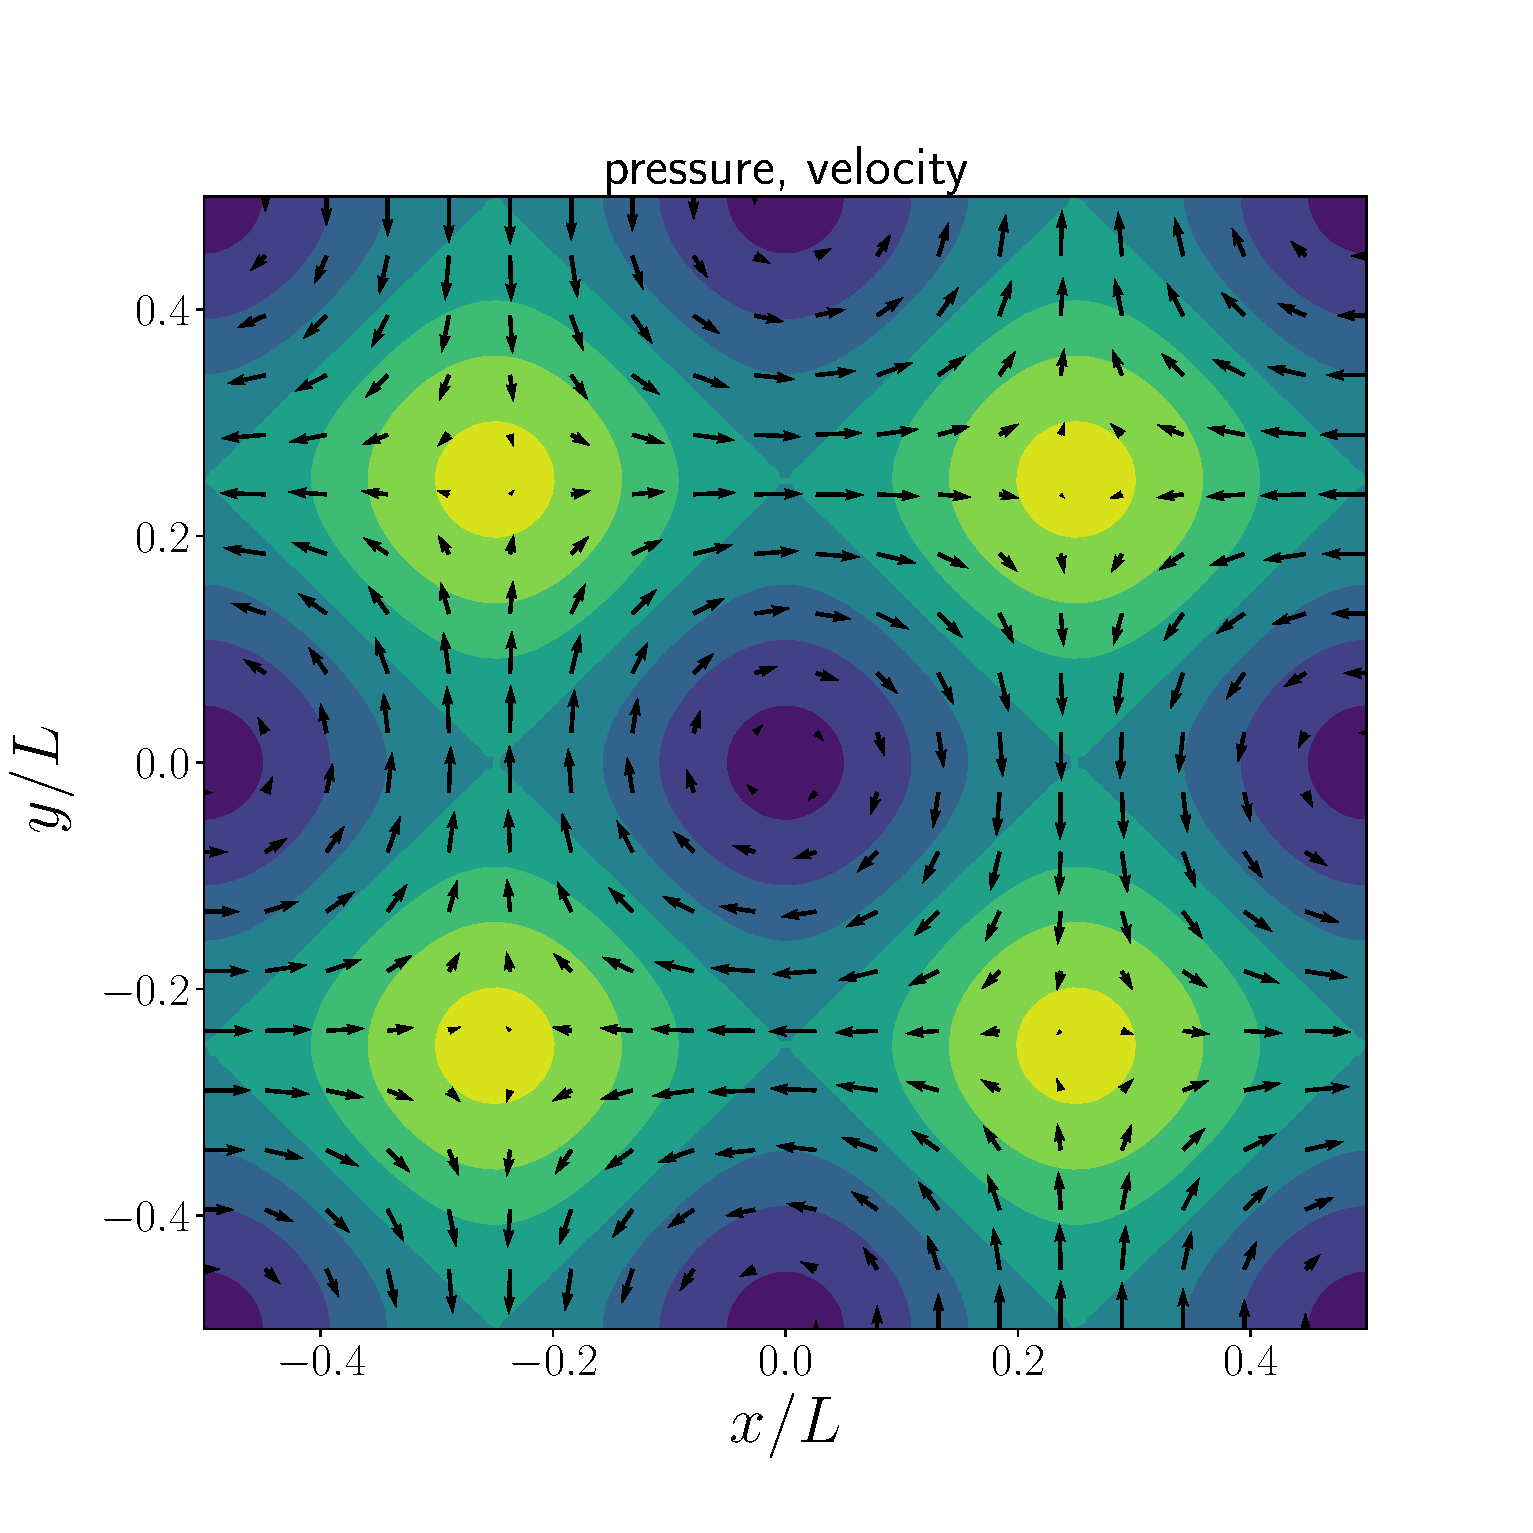
\includegraphics[width=0.4\linewidth]{figures/taylor-green_vortices}
  \caption{Taylor-Green vortices. Contour of iso-pressure (isobars),
    velocity as arrows \label{fig:taylor-green_vortices }}
\end{figure}

Insertion of these two fields into the Navier-Stokes equation shows
that indeed this is a solution. It is interesting that the pressure
gradient term exactly cancels the convective one, while the viscosity
term cancels the partial derivative. That means that in the inviscid
limit the vortices will never decay.

The vorticity field is given by
\[
  \omega = 2 f(t) \sin (kx) \sin (ky)
\]
and the stream function is just $ \psi=\omega /2$. Notice the
vorticity satisfies the convection-diffusion equation
\[
  \frac{d \omega}{d t}= \nu \nabla^2 \omega.
\]



\subsection{Reduced units}

Let us introduce the dimensionless time, built from time, maximum
initial velocity, and typical length $L$ (another choice would be
$L/2$, which is the actual length of a vortex)
\[
  t^*= t u_0 / L.
\]
Notice that $ t^*=1$ is the time a fluid particle would need to travel
a distance $L$.

Function $f$ can be written as
\[
  f(t)= \exp(-2\nu (2\pi/L)^2 (L t^* / L) ) = \exp(-8 \pi^2 t^* / \mathrm{Re}) ,
\]
%
where the Reynolds number appears naturally:
%
\[
  \mathrm{Re} := L u_0 / \nu .
\]

The decay time is then seen to be $ \tau^*=\mathrm{Re}/(8\pi^2)$ in
reduced units.




\section{Attenuation of sound waves*}
\label{sec:sound_waves_att}

This section contains a simple discussion of the role of viscosity in
the attenuation of sound waves. Original work is by Stokes, 1845.

Let us start with the Navier-Stokes momentum equation, which will be
linearized by disregarding high-order deviations from equilibrium
values. The two viscosity coefficients always multiply the velocity
terms. Therefore, they are at to be taken at their equilibrium values,
since any departure would entail higher order terms. This points out
\ref{eq:NS_const_viscs} as our starting point --- even if this case
is not athermal, the fact that the variation of the viscosity
coefficients is neglected leads to the same equation.


After linearizing, the two relevant equations are continuity and
momentum:
\begin{align}
  & \frac{\partial\rho' }{\partial t}  + \rho_0 \divu =0 \\
  & \label{eq:NS_Newtonian_const_visc}
    \rho_0 \frac{\partial \bfu }{\partial t} =
    - c^2 \nabla \rho' + \mu \nabla^2 \bfu
    + ( \mu + \lambda ) \nabla ( \divu ) .
\end{align}
The same assumptions as those in
Eqs. \ref{eq:sound_small_u}-\ref{eq:sound_small_p} have been made.
Also, we write $\kappa = c^2$ for the proportinality of pressure
modulations with density modulations, where $c$ is the sound speed
when viscosity is neglected. The subscript ``$_0$'' is not written for
the viscosity coefficients for simplicity.

Eq. \ref{eq:NS_Newtonian_const_visc} may seem different from previous
expressions, but it is the correct one when $\mu$ is constant, but
incompressibility does not hold. In this case, the term in
\ref{eq:NS_Newtonian} is not zero, but rather gives rise to a
$(\mu + \lambda) \nabla ( \divu )$ term.

Our systems is not as simple as the one in Section
\ref{sec:sound_waves}, where the continuity and momentum equations
where equally simple. There, we could easily eliminate either the
velocity or the density from our equations in order to get a single
equation for the other field. Now, the continuity equation is the
same, but the one for momentum one is much more involved. This leaves
us with eliminating the density as the only viable scheme.

If we apply the gradient operator to continuity, and differentiate
with respect to space in momentum, we arrive to this equation for
the velocity only:
\begin{equation}
  \label{eq:sound_att_Fourier}
  \frac{\partial^2 }{\partial t^2 } \mathbf{u} =
  c^2\nabla \cdot (\divu) + \nu \nabla^2\frac{\partial\bfu}{\partial t} +
  (\zeta - \nu) \nabla (\nabla\cdot \frac{\partial\bfu}{\partial t} ) ,
\end{equation}
where $\nu=\mu/\rho_0$, the usual kinematic viscosity, and we define,
for future convenience, an additional kinematic viscosity
$\zeta=2 \nu+\lambda/\rho_0$.

Clearly, this reduces to our previous sound wave equation if there was
no viscosity.

Let us try a harmonic wave solution of the form
\begin{equation}
  \label{eq:wave_form_visc}
  \bfu = \Re\left[ \bfu_0 e^{i( \beta x - \omega t)} \right].
\end{equation}
Now $\bfu_0$ is a fixed amplitude and polarization vector, which may
be parallel to $\bhe$ in a longitudinal sound wave, but may also be
perpendicular to it, for a traverse wave. In general, of course, a
wave may be a combination of both.

Notice the usage of complex exponentials, which is common in wave
physics. Of course, the actual solution is real, so usually the real
part of the complex solution is kept (sometimes it is the imaginary,
which is equally valid). The flexibility comes partly from the fact
that $\mathbf{u}_0$ could be complex, which would represent a phase.
In our case, this is not important, but rather the possibility that
$\beta$ may be complex. In this case, its values encapsulates both a
real wave number and an spatial decay. Indeed, if
\[
  \beta = k + \alpha i ,
\]
then
\[
  \bfu = \bfu_0e^{- \alpha x} e^{i(k x - \omega t )} ,
\]
which clearly identifies $ \omega=2\pi /\lambda$ as the (real)
wave-number for a wave-lenght $ \lambda$, and $ \alpha=1 /\ell $, as a
sound attenuation coefficient, with $ \ell $ the attenuation length.
\index{sound attenuation coefficient}
\index{attenuation length}

Now, the time derivative is
\[
  \frac{\partial \bfu  }{\partial t }  = -i \omega \bfu ,
\]
and the second derivative,
\[
  \frac{\partial^2 \bfu   }{\partial t^2 }  = -\omega^2 \bfu.
\]

But, it is quite interesting that the two second space derivatives are
not the same. The Laplacian is
\[
\nabla^2 \bfu = -\beta^2 \bfu,
\]
while the gradient of the divergence is
\[
\nabla (\nabla\cdot \bfu ) = -\beta^2 u_x \bhe_x,
\]
where $u_x= \bfu\cdot \bhe_x$ is the longitudinal component of the
sound wave.
%
The latter then acts only on longitudinal waves: tranverse waves are
inherently divergence-free, since depend on one coordinate but point
toward a perpendicular direction (as in Couette and Poiseuille flows).
Let us consider them separately.

\subsection{Longitudinal waves}

In this case, insertion of the wave form \ref{eq:wave_form_visc} into
Eq. \ref{eq:NS_Newtonian_const_visc} yields

\begin{equation}
  -\omega^2 = - c^2\beta^2 + i \zeta  \omega \beta^2 .
\end{equation}
The expression includes the volume bulk viscosity, as seems fitting
for a longitudinal disturbance, which involves compression.  The
appearance of the shear viscosity may come as a surprise \footnote{%
  To be precise, the fact that $\eta$, the volume viscosity, is not
  the only viscosity coefficient that appears, this beign a bit
  obscured by our usage of $\zeta$ instead of $\mu$ and $\eta$.}  The
tensor $\mu$ term in Eq. \ref{eq:pure_stress_pure_compression},
despite being traceless, nevertheless has a non-zero divergence, as
can be easily checked.  This means this wave does not consist of pure
compression, in spite of its appearance: it is also a shear wave (see
Exercises \ref{ex:shear_in_wave} and \ref{ex:div_of_traceless}.)


If viscosities were negligible, the solution is just
\[
\omega =  c \beta ,
\]
%
the usual dispersion relation for sound of
Sec. \ref{sec:sound_waves}. In general, though:
\begin{equation}
  \label{eq:waves_att_dispersion}
  \beta^2 =
  \frac{\omega^2}{c^2 - i \zeta\omega}=
  \frac{\omega^2}{c^2}\frac{1}{1 -  i\omega/\omega_\mathrm{c}},
\end{equation}
where we define the crossover angular frequency \index{crossover
  angular frequency}
\[
  \omega_\mathrm{c} := \frac{c^2}{ \zeta }.
\]

This is the frequency above which the viscosity begins to be relevant.
Numerical values can be found in Table \ref{tbl:sound_att}. The
frequency is really high for the human hearing range, which goes up to
about $\SI{20}{\kilo\hertz}$ for humans. The record in the animal
kingdom is held by porpoises (\ref{fig:porpoises}), but it is only
about $\SI{160}{\kilo\hertz}$. Ultrasonic cleaners used in dentistry
operate at $\SI{40}{\kilo\hertz}$. Medical ultrasound for imaging goes
as high as $\SI{16}{\mega\hertz}$. Only acoustic microscopy
\cite{wiki:AM} reaches a few \si{\giga\hertz}, matching our estimate
for air.


\begin{figure}
  \begin{center}
    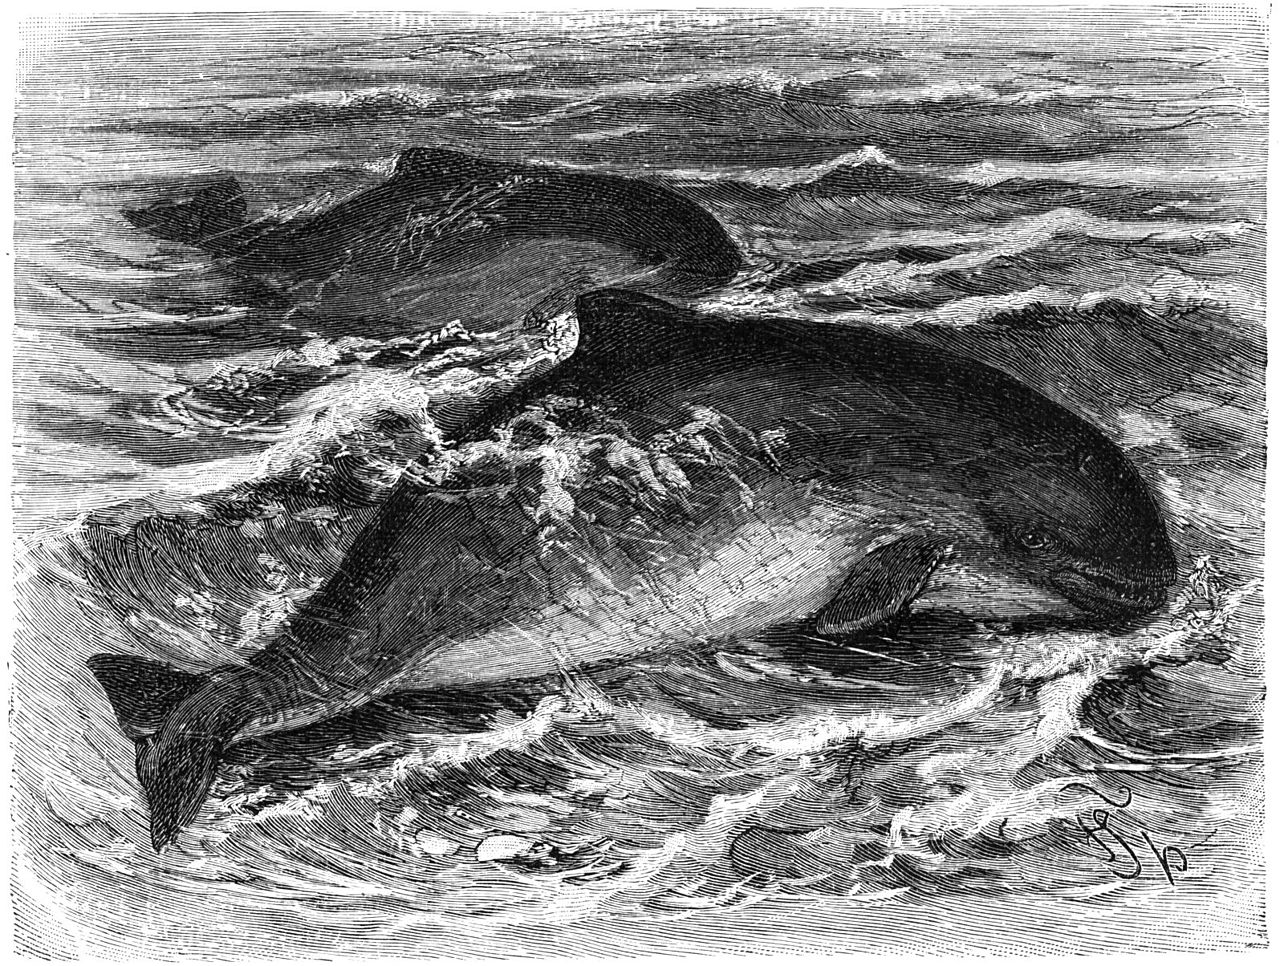
\includegraphics[width=0.7\textwidth]{figures/porpoises}
  \end{center}
  \caption{Harbor porpoises. From \cite{Brehms_Tierleben}.  \label{fig:porpoises}}
\end{figure}


\begin{table}
\begin{tabular}{|c|c|c|c|c|}
  \hline
    & $ c$ (m/s) &  $ \nu$ (m$^2$/s) & $\lambda$ (m$^2$/s) & $ f_\mathrm{c}$ (GHz)\\
  \hline
  \hline
  water (15$^\circ$C) & $1480$& $ 1.13 \times 10^{-6}$ & $ 3.1 \times 10^{-6}$ & $68$ \\
  \hline
  air & $340$   & $ 1.48\times 10^{-5}$ & $ 5 \times 10^{-6}$ ? & $0.5$ \\
  \hline
\end{tabular}
\caption{Numerical values for two important substances. Values with
  question marks are speculative, since in Cramer\cite{Cramer} air is
  said to have a negligible bulk viscosity\ldots but in a graph this
  quantity's value is seen to be about half the shear viscosity value,
  and air is mostly nitrogen.
 \label{tbl:sound_att}}
\end{table}

It is somewhat tedious to find the real and imaginary parts of $\beta$
from Eq. \ref{eq:waves_att_dispersion} (the general solution is shown
in Figure \ref{fig:sound_wave_att}.)  The resulting expressions are,
moreover, not very iluminating except at low and high frequencies
(with respect to $\omega_\mathrm{c}$). We find it better then to study
these two limits from approximations to
Eq. \ref{eq:waves_att_dispersion}, and leave the general solution as
Exercise \ref{ex:sound_att}, for the interested reader.

\begin{figure}
  \centering
  \begin{minipage}{0.7\textwidth}
      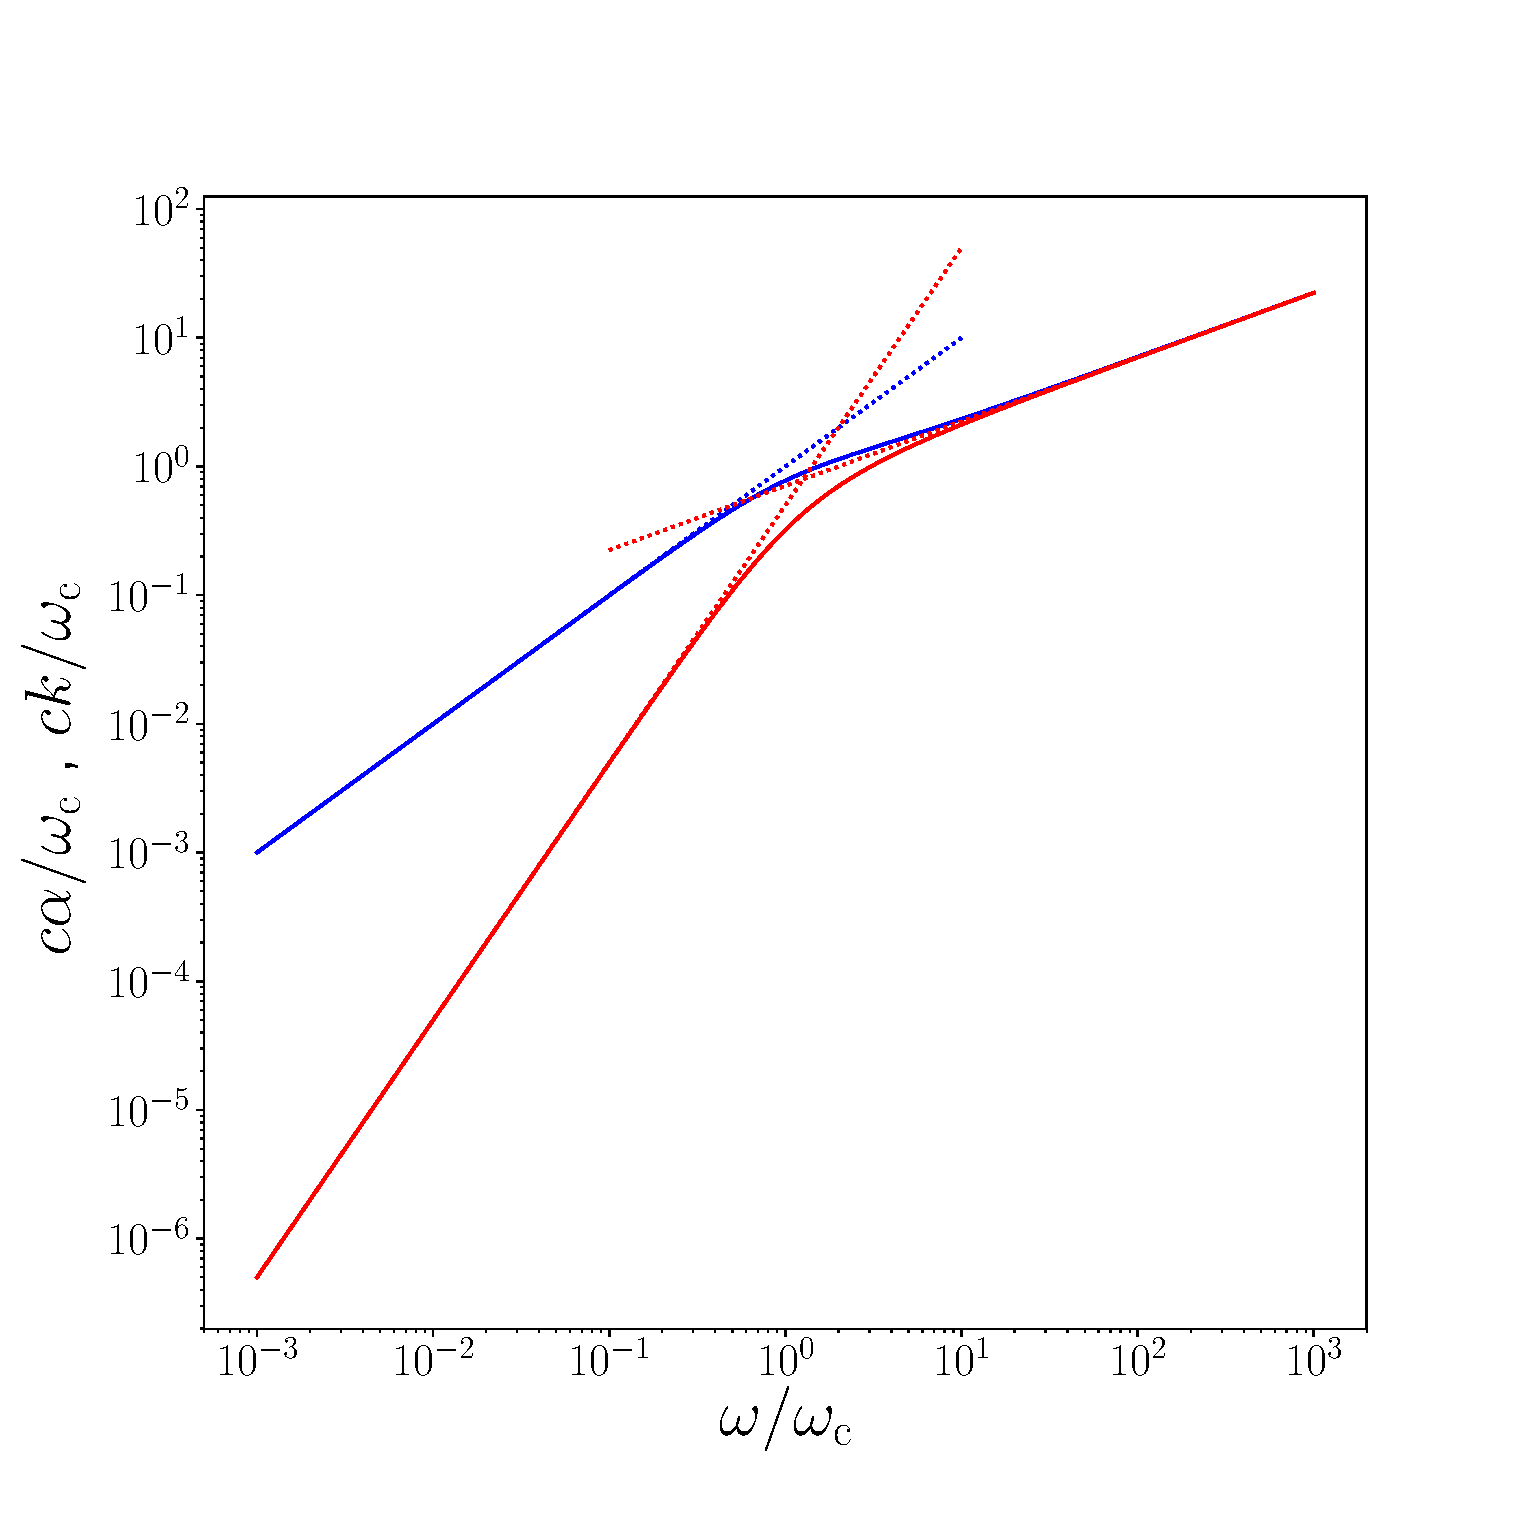
\includegraphics[width=\textwidth]{figures/sound_wave_att}
  \end{minipage}
  \caption{Plot of reduced wave-vector, $k c /\omega_\mathrm{c}$ (blue), and
    attenuation coefficient, $\alpha c /\omega_\mathrm{c}$ (red), as functions
    of reduced frecuency $\omega /\omega_\mathrm{c}$. Dotted lines are
    assymptotic regimes at low and high frequencies.
    \label{fig:sound_wave_att}}
\end{figure}


\subsubsection{Low frequencies}


At frequencies much below the crossover frequency, we may expand the
term in the denominator in a Taylor series, then again for the square
root. The end result is
\[
\beta = \frac{\omega}{c} \left(1 + i   \frac{\omega}{2 \omega_\mathrm{c}}\right).
\]
%
Therefore, the wave number is
\[
\beta = \frac{\omega}{c},
\]
as if there were no viscosity (this corresponds to the dotted blue
line at low frequencies in Figure \ref{fig:sound_wave_att}).

The attenuation coefficient is
\[ \alpha = \frac{\omega^2}{2 c\omega_\mathrm{c}}=
\frac{ \zeta \omega^2 }{2 c^3}. \]
%
It therefore grows as the square of the frequency (red dotted blue
line at low frequencies in Figure \ref{fig:sound_wave_att}).  This
agrees is called ``Stokes' law of sound'' \index{Stokes' law of
  sound}. Notice that the alternative form is often found
\cite{wiki:SLoSA}:
\[
  \alpha =  \frac{\omega^2}{\rho_0 c^3}
  \left( \frac23 \mu+ \frac12 \eta  \right),
\]
with $\eta= (2/3) \mu + \lambda$ the volume compressiblity.

This means that for that the highest sound in a porpoise's range, at
$\SI{160}{\kilo\hertz}$ the attenuation length would be about
$\SI{8}{\kilo\meter}$ (in water, of course). This may be important for
the long-range communication of these animals. For medical ultrasound
at $\SI{16}{\mega\hertz}$ this length is
$\approx\SI{80}{\centi\meter}$, with water values (a fair
approximation for the human body.) This can have an impact for human
tissues, in the sense that in a distance of some tens of centimeters
the energy of the ultrasound waves is dissipated inside the body of
the patient, and may cause unwanted heating.

\subsubsection{High frequencies}

At frequencies much higher than the crossover, we may neglect the
``1'' in the denominator of \ref{eq:waves_att_dispersion}, to obtain
\[
\beta^2 = \frac{i \omega\omega_\mathrm{c}}{c^2} .
\]
If we substitute the crossover frequency:
\[
\beta^2 = \frac{\omega}{i \zeta} =\frac{i \omega}{\zeta} 
\]
Recalling $i = e^{(pi/2)i} $, the solution is
\[
\beta =\sqrt{ \frac{\omega}{ \zeta }} e^{(\pi/4)i}.
\]

Therefore
\[
k=\alpha =\sqrt{\frac{\omega}{ 2 \zeta}}.
\]

This is an interesting result, since the attenuation coefficient is
equal to the wave number (dotted black line at high frequencies in
Figure \ref{fig:sound_wave_att}).

The attenuation length is
\[
\ell= \frac{1}{\alpha}=\sqrt{\frac{ 2 \zeta}{\omega}}
\]
The function looks therefore like a simple function
\[
g(x)= f(x/\ell) \qquad  f(x) = e^{-x}\cos(x) .
\]
In Figure \ref{fig:expcos}, it is seen to decay very fast, with just
one maximum of minimum of importance.

\begin{figure}
  \begin{center}
    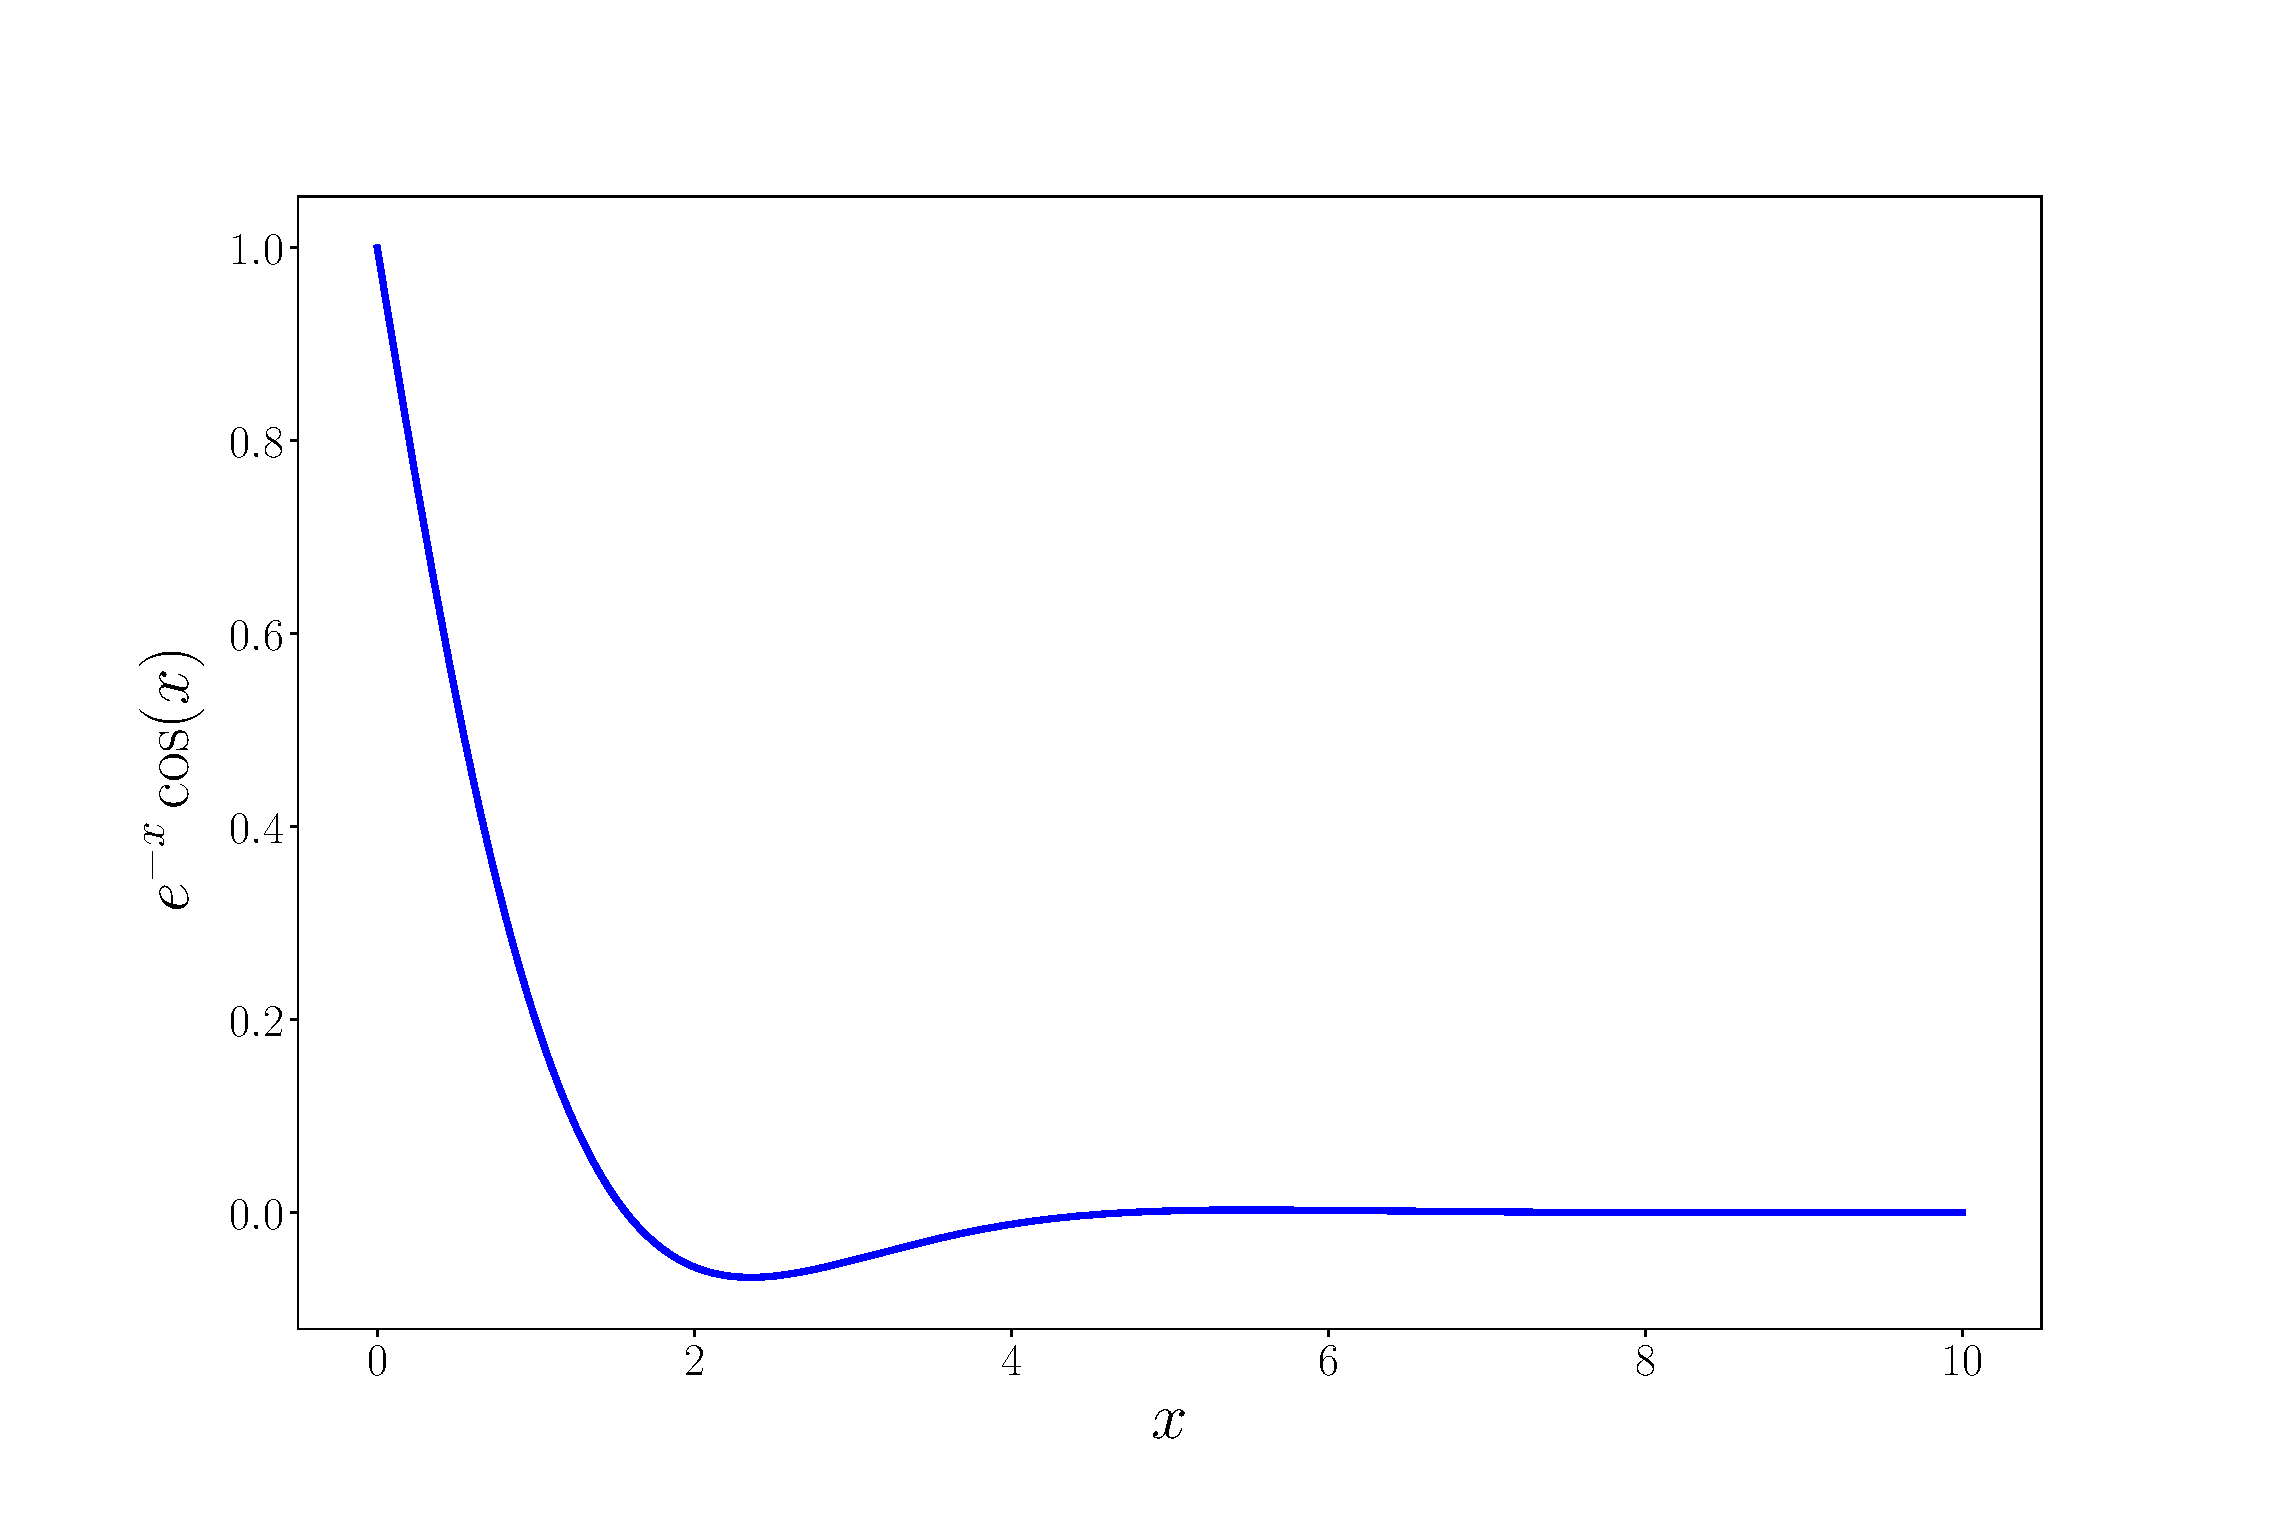
\includegraphics[width=0.7\textwidth]{figures/expcos}
  \end{center}
  \caption{Graph of the function $e^{-x}\cos(x)$ \label{fig:expcos}}
\end{figure}
 



\subsubsection{At the crossover frequency}

A fast check on the above approximations is to see what happens when
the frequency is exactly the crossover frequency. At this point, the
growth of the attenuation coefficient as the square of frequency
crosses over to a growth as the square root. This would mean a bend in
a log-log plot, between two straight lines with different slopes. This
is indeed apparent in Figure \ref{fig:sound_wave_att}.

The extrapolation of the low frequency expression yields
\[
\alpha_\mathrm{c}\approx \frac{\omega_\mathrm{c}}{2 c} ,
\]

whereas the high frequency expression yields
\[
\alpha_\mathrm{c}\approx \frac{\omega_\mathrm{c}}{\sqrt{2} c} ,
\]
which are similar.

The exact expression can be shown to be, after some involved algebra,
\[
\alpha_\mathrm{c} =\frac{ \sin(\pi/8) \omega_\mathrm{c} }{ (2^{1/4} c } ,
\]
a value just a bit below the other two. This means the approximations
remain quite fair up to the limit of their respective ranges.

By the way, for water this value corresponds to an attenuation length
of about \SI{10}{\nano\meter}, which is a really short length, in the
atomic range. For air, it is about \SI{0.3}{\micro\meter}, the size of
a very small cell.

\subsection{Transverse waves}

We tend to think sound waves are longitudinal. We here discuss how
they may have a transverse component, but it is dampened at al
frequencies.

If we write Eq. \ref{eq:sound_att_Fourier} for the $y$ or $z$
Cartesian component, we find
\[
-\omega^2 =  i \nu \omega \beta^2 ,
\]
or
\[
\beta^2 = \frac{i \omega}{\nu}.
\]
Only $\nu$ is involved, which is sensible: transverse waves do involve
only shear, not compression (at variance with longitudinal waves,
which involve both.)

The expression is very similar to the one for longitudinal waves at
high frequencies, only this one is valid at \emph{all} frequencies.
Its solution is
\[
k = \alpha = \sqrt{ \frac{\omega}{ 2 \nu}}.
\]
Figure \ref{fig:expcos} still applies to these waves, with the
difference that the decay length is
\[
\ell= \frac{1}{\alpha}=\sqrt{\frac{ 2 \nu}{\omega}}
\]

For frequencies of ordinary ``sound'', i.e. audible frequencies, that
length is quite small. With the numerical data in the Table, that
length is only about \SI{0.7}{\milli\meter} for air, at a very low
frequency of \SI{10}{\hertz} (just below the lower hearing threshold),
and will decrease further as the inverse of the square root of the
frequency.



\section{Fourier space}

In Fourier space all the fields are given as \index{Fourier transform} of their Fourier components:
\begin{equation}
	\label{eq:F_q_to_r}
	\phi(\bfr) = \frac 1{(2\pi)^d}  \int d\bfq \, \phi(\bfq) e^{ i\bfq\cdot\bfr} .
\end{equation}
In some settings, this integral may be replaced by a sum over integer-labeled Fourier components
(and is therefore termed a Fourier series.)
Notice that in this section Fourier components are indicated by their arguments taking a wave-vector. This is not too elegant, and a tilde (``wiggly'')
hat should be used for them.

The Fourier components can be obtained by the direct Fourier transform:
\begin{equation}
	\label{eq:F_r_to_q}
	\phi_\bfq =                    \int d\bfr \, \phi(\bfr) e^{-i\bfq\cdot\bfr}  
\end{equation}

In the incompressible Navier-Stokes equation \eqref{eq:NS_usual}, the viscous and force terms are trivial in Fourier space, giving
\begin{equation*}
	\frac{\partial}{\partial_t} \mathbf{u} (\mathbf{k}) + \mathbf{a}(\mathbf{k}) =
	-[\nabla p ](\mathbf{k}) - \nu k^2 \mathbf{u}(\mathbf{k}) + \mathbf{f}(\mathbf{k}) ,
\end{equation*}
where $\mathbf{a}$ stands for the convective acceleration, $ \mathbf{a} := (\mathbf{u}\cdot\nabla)\mathbf{u} $. Ignoring, and the pressure, the Fourier modes are decoupled. For example, starting from a null velocity field, the solution is
readily obtained as
\begin{equation} \label{eq:Fourier_simple_solution}
	\mathbf{u} (\mathbf{k}, t ) =
	\frac{\mathbf{f}(\mathbf{k})}{\nu k^2}
	\left[ 1-  \exp \left( - \nu k^2 t  \right)   \right]  .
\end{equation}

This shows that the final velocity is given by $\mathbf{f}(\mathbf{k}) / \nu k^2 \sim  \mathbf{f}(\mathbf{k}) \lambda^2 / \nu $, so that longer wavelengths are more affected by a force.
Also, the typical relaxation time of a mode is given by $\tau= 1/( \nu k^2 ) \sim \lambda^2 / \nu$, so longer wavelengths take longer to reach equilibrium.



\subsection{Convective acceleration in Fourier space}

From its definition \(
\mathbf{a} := (\mathbf{u}\cdot\nabla)\mathbf{u} ,
\)
%
\[
\mathbf{a} = 
\left(
\sum_\mathbf{p} \mathbf{u}(\mathbf{p} ) e^{\mathi \mathbf{p}\cdot\mathbf{r}} 
\cdot\nabla
\right)
\sum_\mathbf{q} \mathbf{u}(\mathbf{q} ) e^{\mathi \mathbf{q}\cdot\mathbf{r}} .
\]

It is clearer perhaps in Fourier component form:
\[
a_i = 
\sum_\mathbf{p} u_j(\mathbf{p} )  e^{\mathi \mathbf{p}\cdot\mathbf{r}} 
\partial_j
\sum_\mathbf{q} u_i(\mathbf{q} ) e^{\mathi \mathbf{q}\cdot\mathbf{r}} ,
\]
where Einstein's summation convention is used. Also, $\mathi$ is used
for the imaginary unit, since the letter $i$ is used as an index for
Cartesian components. Then,
\[
a_i = \mathi
\sum_{ \mathbf{p}, \mathbf{q}}
u_j(\mathbf{p} )
q_j
u_i(\mathbf{q} )
e^{\mathi ( \mathbf{p}  +  \mathbf{q} ) \cdot\mathbf{r}} ,
\]
or
\[
\mathbf{a} = \mathi
\sum_{ \mathbf{p}, \mathbf{q}}
(\mathbf{u}(\mathbf{p} )
\cdot
\mathbf{q})
\mathbf{u}(\mathbf{q} )
e^{\mathi ( \mathbf{p}  +  \mathbf{q} ) \cdot\mathbf{r}} .
\]

The Fourier components will be given by \eqref{eq:F_q_to_r}, and by orthogonality of the
complex exponential functions:
\[
\mathbf{a}(\mathbf{k})= \mathi
\sum_{ \mathbf{p} + \mathbf{q} = \mathbf{k}}
(\mathbf{u}(\mathbf{p} )
\cdot
\mathbf{q})
\mathbf{u}(\mathbf{q} ) .
\]
This is a \emph{single} sum: for a given $\mathbf{k}$ we sum over all $\mathbf{p}$,
with $\mathbf{q}$ fixed by the sum rule $\mathbf{p} + \mathbf{q} = \mathbf{k}$.

Clearly, the convective acceleration is responsible for the coupling of the different Fourier modes.


Also, since $\mathbf{p} \cdot \mathbf{u}(\mathbf{p}) = 0$ by incompressibility, we
may change $\mathbf{q}$ to $\mathbf{q} + \mathbf{p} = \mathbf{k} $,
so
\[
\mathbf{a}(\mathbf{k})=\mathi
\sum_{ \mathbf{p} + \mathbf{q} = \mathbf{k}}
(\mathbf{u}(\mathbf{p} )
\cdot
\mathbf{k})
\mathbf{u}(\mathbf{q} ).
\]
The term $\mathbf{k}$ can be taken out of the summation, but it is awkward in vector form. Not so in components:
\[
a_i(\mathbf{k})=\mathi
k_j
\sum_{ \mathbf{p} + \mathbf{q} = \mathbf{k}}
u_j (\mathbf{p} )
u_i(\mathbf{q} ) .
\]



\subsection{Pressure in Fourier space}

Taking the divergence of the Navier-Stokes equation, \eqref{eq:NS_usual}, and applying incompressibility,
\begin{equation}\label{eq:Poisson}
	\nabla\cdot \mathbf{a} = -\nabla^2 p + \nabla\cdot \mathbf{f} ,
\end{equation}
which is the \index{Poisson pressure equation} (PPE).
In principle, this equation can be solved in real space, obtaining the pressure from it. Introducing its gradient back into \eqref{eq:NS_usual} the Navier-Stokes equation this is a possible way to solve the problem. (Indeed, this is the procedure in some computational algorithms.)

In Fourier space,
\[
-k^2 p (\mathbf{k} ) = - \mathi \mathbf{k} \cdot \mathbf{a}(\mathbf{k}) + \mathi \mathbf{k} \cdot \mathbf{f}(\mathbf{k}) ,
\]
or
\[
p (\mathbf{k} ) =  \frac{\mathi}{k^2} \mathbf{k} \cdot \mathbf{a}(\mathbf{k})
- \mathi \frac{\mathbf{k} \cdot \mathbf{f}(\mathbf{k})}{k^2}  .
\]


Hence,
\begin{align*}
	p (\mathbf{k} ) & = -\frac{1}{k^2} 
	\sum_{ \mathbf{p} + \mathbf{q} = \mathbf{k}}
	(\mathbf{u}(\mathbf{p} )
	\cdot
	\mathbf{k}
	)
	(
	\mathbf{u}(\mathbf{q} ) \cdot
	\mathbf{k}
	) 
	- \mathi
	\frac{\mathbf{k} \cdot \mathbf{f}(\mathbf{k}) }{k^2}     
	%\\
	%&= -\frac{1}{k^2} 
	%\left[
	%\sum_{ \mathbf{p} + \mathbf{q} = \mathbf{k}}
	%(\mathbf{u}(\mathbf{p} )
	%\cdot
	%\mathbf{k}
	%)
	%(
	%\mathbf{u}(\mathbf{q} ) \cdot
	%\mathbf{k}
	%) 
	%+ \mathi
	%(\mathbf{k} \cdot \mathbf{f}(\mathbf{k}) )
	%\right]
\end{align*}


Or, in components,
\[
p (\mathbf{k} ) = -\frac{k_j k_m}{k^2}
\sum_{ \mathbf{p} + \mathbf{q} = \mathbf{k}}
u_j(\mathbf{p} )
u_m(\mathbf{q} )
- \mathi
\frac{k_j f_j(\mathbf{k}) }{k^2} .
\]


The NS equation features the pressure gradient, which will be given in Fourier space as:
\[
[\nabla p ](\mathbf{k}) = \mathi \mathbf{k} p(\mathbf{k}) .
\]

I.e.
\[[\nabla p ](\mathbf{k}) =
-\mathi \frac{\mathbf{k} }{k^2} 
\sum_{ \mathbf{p} + \mathbf{q} = \mathbf{k}}
(\mathbf{u}(\mathbf{p} )
\cdot
\mathbf{k}
)
(
\mathbf{u}(\mathbf{q} ) \cdot
\mathbf{k}
) 
+ \mathbf{k}
\frac{\mathbf{k} \cdot \mathbf{f}(\mathbf{k})  }{k^2} 
\]




\subsection{Assembly of the final equation}


Recalling our previous expressions for the convective acceleration and pressure,
\begin{equation*}
	\partial_t \mathbf{u} (\mathbf{k})  =
	- \mathi  
	\sum_{ \mathbf{p} + \mathbf{q} = \mathbf{k}}
	(\mathbf{u}(\mathbf{p} ) \cdot \mathbf{k} )
	\left[ 
	1 - \mathbf{k} \frac{\mathbf{k} }{k^2} \cdot 
	\right]
	\mathbf{u}(\mathbf{q} )
	%
	- \nu k^2 \mathbf{u}(\mathbf{k}) +
	\left[ 
	1 - \mathbf{k} \frac{\mathbf{k} }{k^2} \cdot 
	\right]
	\mathbf{f}(\mathbf{k}) .
\end{equation*}

In component form,
\begin{equation*}
	\partial_t u_i (\mathbf{k})  =
	- \mathi  k_m
	\left[ 
	\delta_{ij} - \frac{k_i k_j  }{k^2}
	\right]
	\sum_{ \mathbf{p} + \mathbf{q} = \mathbf{k}}
	u_j(\mathbf{p} ) u_m(\mathbf{p} ) 
	- \nu k^2 u_i(\mathbf{k}) +
	\left[ 
	\delta_{ij} - \frac{k_i k_j }{k^2} 
	\right]
	f_j(\mathbf{k}) .
\end{equation*}

Notice the appearance of the operator \(  \delta_{ij} - k_i k_j  / k^2 \) in both the
term coupling the velocities in different modes, and in the external force. In both cases,
\(  \delta_{ij} \) represents a straight correspondence, while \(  - k_i k_j  / k^2 \)
is a term brought about by the pressure.



\section{Exercises}

\begin{enumerate}

	\item Prove the expression for the unsteady Couette flow.
	
	\item \label{ex:shear_in_wave} Write down the pure-shear stress tensor
	(see also Eq. \ref{eq:pure_stress_pure_compression}):
	\[
	\tau_\mathrm{ps} :=
	\mu  \left[
	\left(
	\nabla\bfu + \nabla\bfu\tran  - \frac23 (\divu)  \eye
	\right)
	\right] 
	\]
	for our linear wave \ref{eq:wave_form_visc} in the case it is
	longitudinal. Show that it is traceless (which it must, by
	definition), but non-zero. This latter fact indicates that our wave
	is not purely compressive in nature.
	
	\item \label{ex:div_of_traceless} Show that the volumetric force due
	to the previous pure-stress is
	\[
	\mu \nabla \cdot  \tau_\mathrm{ps}  = -\frac43 \mu \beta^2 \bfu
	\]
	
	\item \label{ex:sound_att} Find the general solution of
	Eq. \ref{eq:waves_att_dispersion} for the real and imaginary parts
	of $\beta$. Hint: use reduced quantities $\beta'= c\beta/\omega $,
	$\omega'=\omega/\omega_\mathrm{c}$, in terms of which the equation
	reads simpler:
	\[
	\beta'^2 = \frac{1}{1-i \omega'} .
	\]
	Then, write $\beta'=k'+i \alpha'$, find its square, and equate real
	and complex parts on both sides of the equation.  The solution is
	\begin{align*}
		2\alpha'^2 &=\frac {1}{\sqrt{1+\omega'^{2}}} - \frac {1}{1+\omega'^{2}} \\
		2k'^2     &=\frac {1}{\sqrt{1+\omega'^{2}}} + \frac {1}{1+\omega'^{2}}
	\end{align*}
	
	
\end{enumerate}

\chapter{The overdamped limit}

The low Reynolds number is called the creeping, or over-damped
regime. Let us generalize slightly the momentum equation
Eq \ref{eq:NS_usual} to a general volumetric external force $\bff$:
\[
  \rho \frac{d\bfu }{dt} =
  - \nabla p 
  + \mu \nabla^2 \bfu
  + \bff .
\]

We may again cast the equation into reduced form, to get
\[
\rho^* \frac{d\bfu^* }{dt^* } =
-  \nabla^* p^*
+  \frac1\mathbf{Re} \nabla^{*2} \bfu^* .
+  \bff^* ,
\]
where $\bff^*= L/(\rho_0 u_0^2) \bff$. 

As $\mathbf{Re}$ is very small, the equation will tend to
\[
0 = - \mathbf{Re} \nabla^* p^* + \nabla^2 \bfu^* + \mathbf{Re} \bff^*
.
\]
All time derivatives are gone from the equation! The only time
variation that is sometimes considered is the case in which $\bff^*$
is a explicit function of time. In this case, the velocity field
addapts



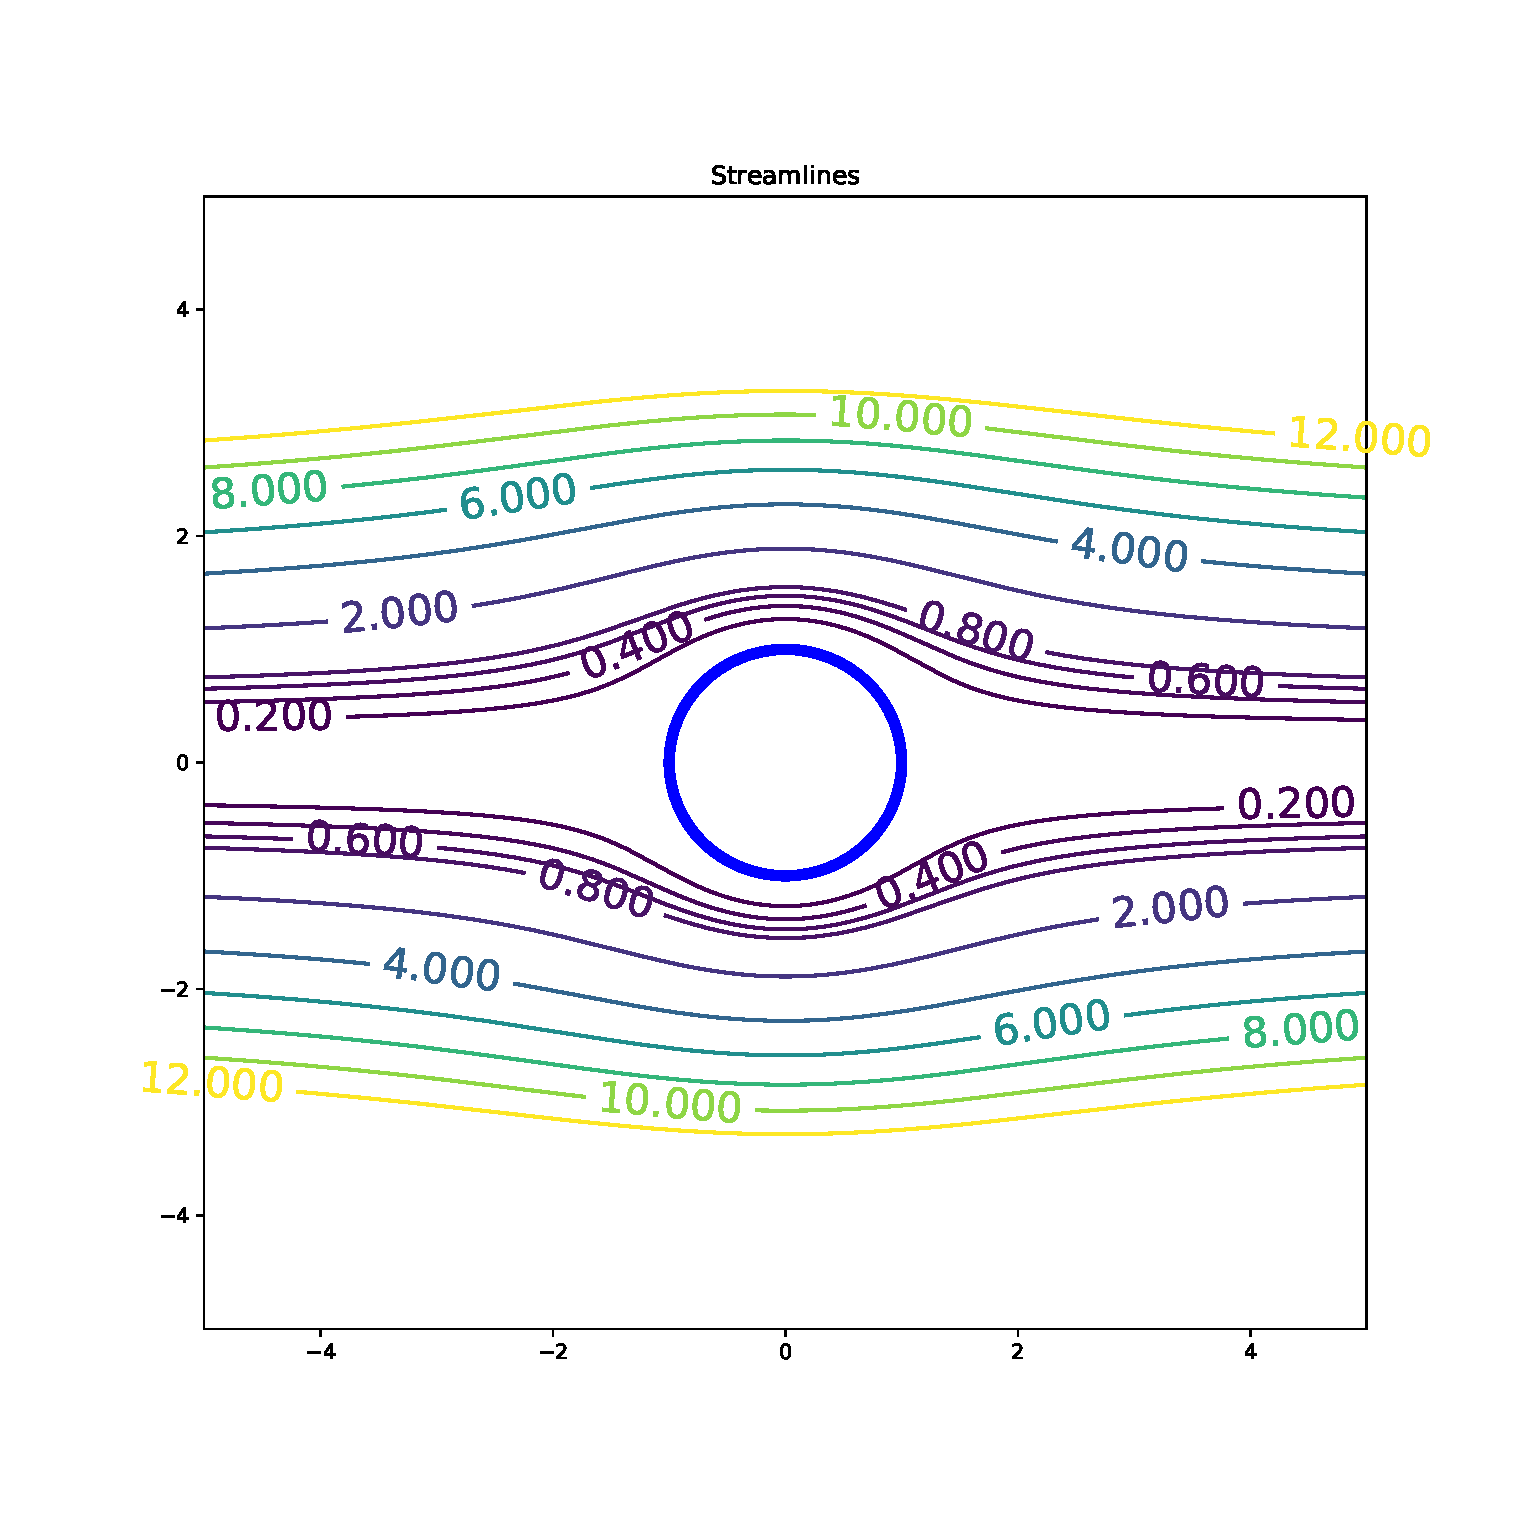
\includegraphics[width=0.8\linewidth]{figures/creeping_flow_past_sphere}

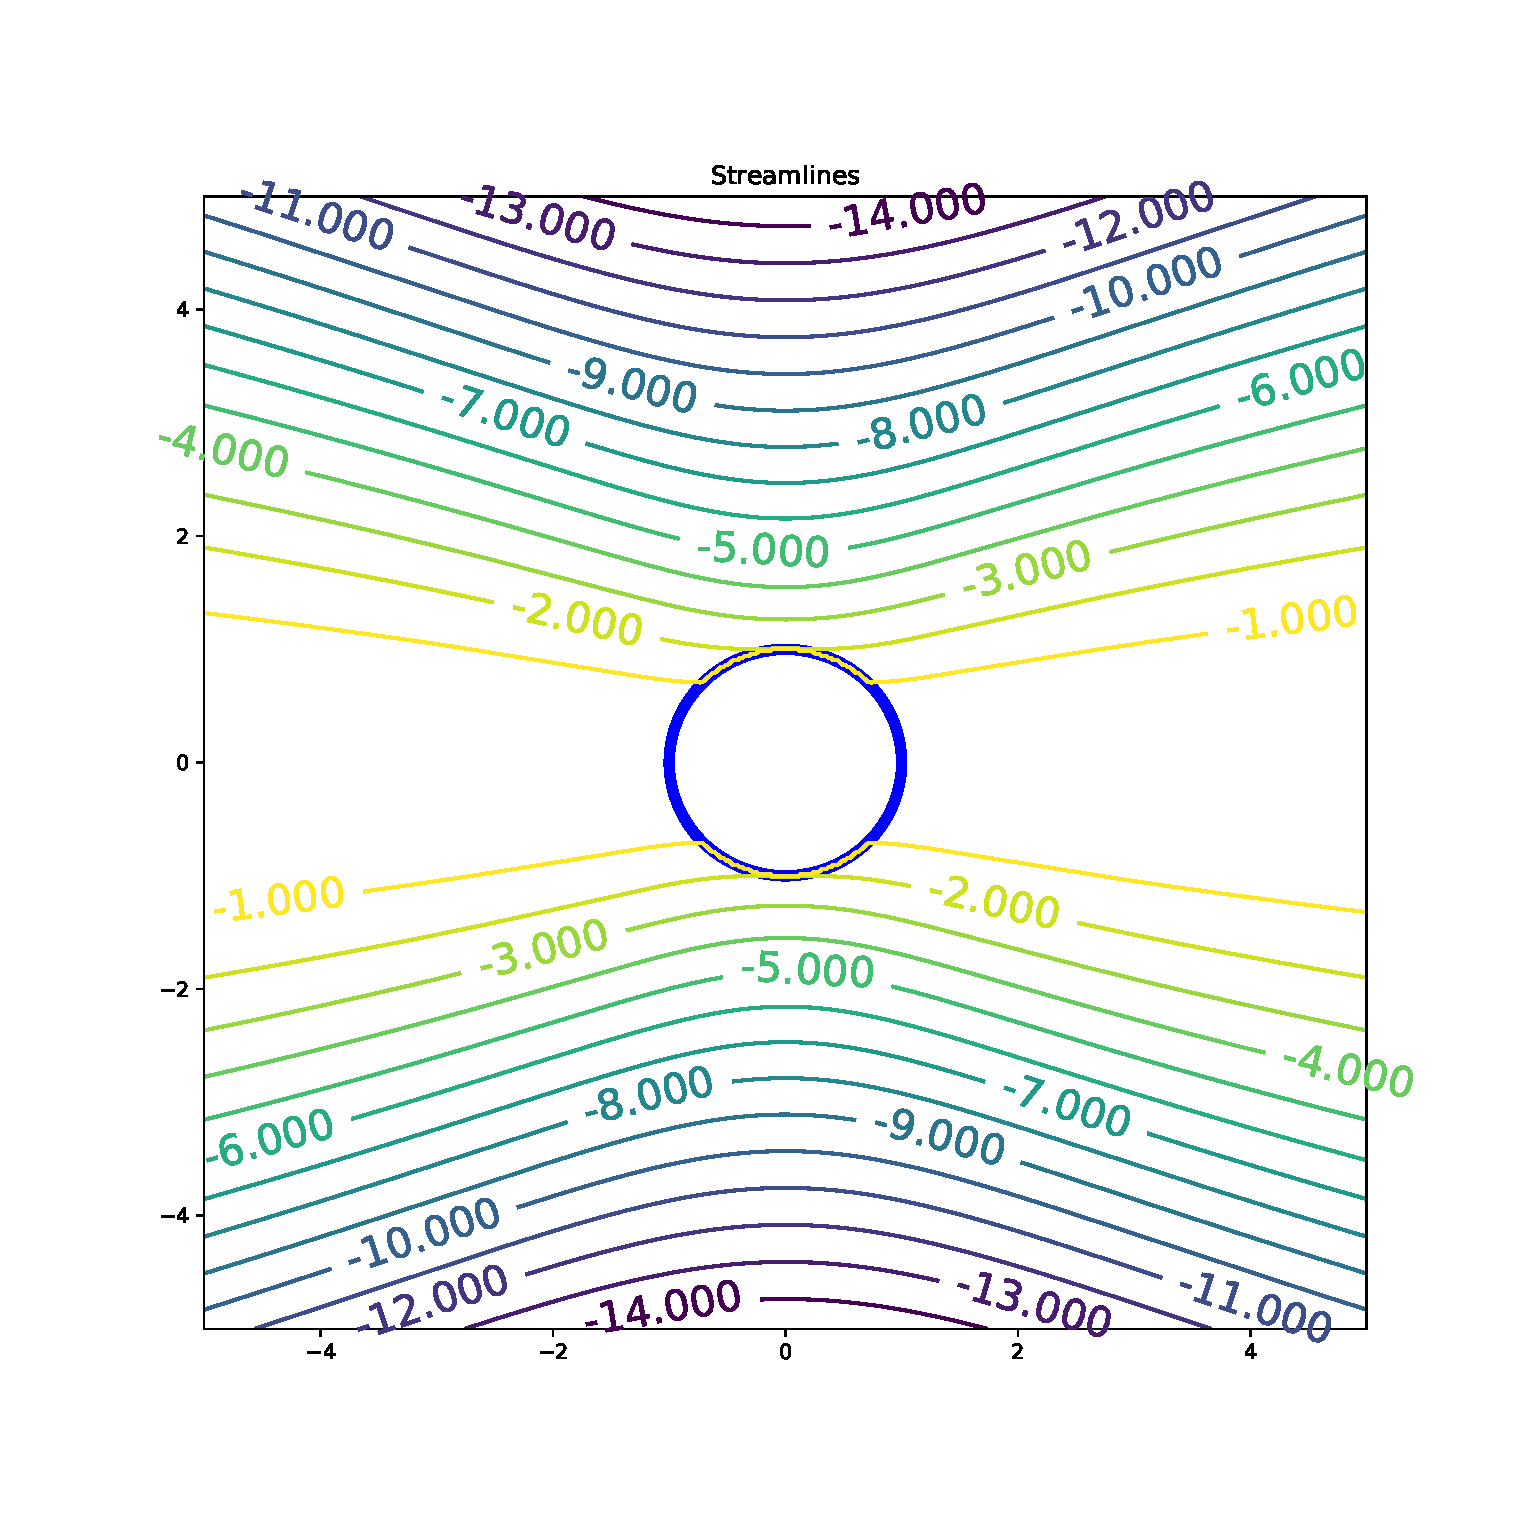
\includegraphics[width=0.8\linewidth]{figures/creeping_flow_past_sphere_moving}







\subsection{Kolmogorov flow}

In order to get an idea of the features of the flow (typical speed,
time scale, Reynolds number), we may gain some insight from the
solution from Kolmogorov flow.

This is an exact solution of the momentum equations when there is a
periodic applied force in the $x$ direction that depends on $y$ only
\[
\bff = f_0 \cos(2\pi y/L) \mathbf{e}_x .
\]

In this case, the typical lengthscale $L_0$ and velocity $u_0$ are set
by the force. The former is clearly $L_0=L$, but the velocity is
actually part of the solution. It is therefore more convenient to
introduce an alternative way to cast the momentum equation in
non-dimensional form. First, dividing by $f_0$ and going to
dimensionless spacial coordinates:
\begin{equation}
\label{eq:Navier-Stokes_nondim1}
\frac{\rho}{f_0}
\frac{d \bfu}{d t} =
\frac\eta{f_0 L^2} (\nabla^*)^2 \bfu
-\frac 1{f_0 L} \nabla^* p + \bff^*(\bfr^*) .
\end{equation}
The viscous term sets the velocity scale: $u_0 = ( f_0 L^2 ) / \eta $.
On the left hand side the total derivative limits the setting of the
time scale. Indeed, $t_0=L/u_0$, or else the two terms in the
derivative, Eq. \ref{eq:total_deriv}, have different scaling. (This
may be alright in theory, and in an Eulerian simulation, but in a
Lagrangian simulation it is not, since the advection term does not
appear explicitely.) This means the equation may be written as
\[
\frac{\rho L^3 f_0}{\eta^2}
\frac{d \bfu^*}{d t^*} =
(\nabla^*)^2 \bfu^*
-\nabla^* p^* + \bff^*(\bfr^*) ,
\]
or
\begin{equation}
\label{eq:Navier-Stokes_nondim2}
\mathrm{Re}
\frac{d \bfu^*}{d t^*} =
(\nabla^*)^2 \bfu^*
-\nabla^* p^* + \bff^*(\bfr^*) ,
\end{equation}
where we again find the Reynolds number, given as $\rho L^3 f_0 /
\eta^2$.  Notice that the reduced response time is given by the
Reynolds number: a high Reynolds number means a long reduced time to
respond, while a low Reynolds one the response is very rapid, and the
equilibrium solution is reached very fast.

To summarize, the various scales are given by:
\begin{itemize}
\item force $f_0$
\item space $L$ (therefore, the reduced del operator $\nabla^* :=
  L \nabla$),
\item velocity $u_0 = ( f_0 L^2 ) / \eta $,
\item time $t_0 = L / u_0 = \eta / (f_0 L) $,
\item pressure $p_0= f_0 L $,
\item the Reynolds number is Re=$\rho L^3 f_0 / \eta^2$
\end{itemize}


Let us apply this scaling to the Kolmogorov flow. The starting
equation for the $x$ component of the velocity, called customarily
``$u$'' is:
\begin{equation}
\label{eq:Kolmo_orig}
  \rho \frac{\partial u}{\partial t} =
  \eta \nabla^2 u - \nabla p +   f_0 \cos(2\pi y/L)  .
\end{equation}

We have supposed that the resulting velocity, as the driving force,
only has an $x$ component varying on $y$, so that the convective term
is zero. In this case, the flow is always incompressible
($\nabla\cdot\bfu =0$), so we may set the pressure to some constant
values, which thus disappears from the equation, which is just:
\[
  \rho \frac{\partial u}{\partial t} =
  \eta \nabla^2 u +   f_0 \cos(2\pi y/L)  .
\]

In reduced units (dropping the asterisks for clarity), this is
\[
  \mathrm{Re} \frac{\partial u}{\partial t} = \nabla^2 u + \cos(2\pi y) .
\]

The solution is easily found:
\[
u = \frac{1}{(2\pi)^2} \left( 1-e^{ - (2\pi)^2 t/Re } \right)  \cos(2\pi y) .
\]

Putting the scales back in, we find
\[
u = \frac{ f_0 L^2 }{(2\pi)^2 \eta}
\left( 1-e^{- (2\pi)^2 \eta  t / (\rho L^2) } \right)  \cos(2\pi y/L) ,
\]
which indeed is the solution to the original Equation
\ref{eq:Kolmo_orig}.


\section{Around Stokes paradox*}
\label{sec:creeping_cylinder}

Stokes paradox is very soon encountered. Our task is to solve the
bi-Laplace equation, Eq. \ref{eq:bi-laplacian}, for a 2D case, in
which the vector potential $\bfA$ only has a $z$ component, equal
to the stream function $\psi$. Then,
\[
  \nabla^4 \psi = 0 ,
\]
from which $u=\nabla\times\psi$. Finally, the pressure field is
obtained from Stokes equation, \ref{eq:Stokes}:
$\nabla p = \mu \nabla^2 \bfu$.

In polar coordinates,
\begin{equation}
  \label{eq:Lapl_in_polar}
  \nabla^2 \psi =
  {1 \over  r}{\partial \over \partial  r}\left(
    r {\partial f \over \partial  r}\right)
  + {1 \over  r^2}{\partial^2 f \over \partial \theta^2} .
\end{equation}

Trying a function $\psi = r^\alpha \sin\theta$, we find that
\begin{equation*}
  \nabla^2   r^\alpha \sin\theta  =
  r^{\alpha-2} \sin\theta \left( \alpha^2 -1  \right) .
\end{equation*}

This means the only two possibilities are $\alpha=\pm 1$. Indeed, the
potential solution for the flow past a cylinder was built from these
two solutions (see e.g. Eq \ref{eq:pot_phi_guess}).

The bi-Laplacian is then
\begin{equation*}
  \nabla^4   r^\alpha \sin\theta  =
  r^{\alpha-4} \sin\theta
  \left( \alpha^2 -1  \right)
  \left( (\alpha-2)^2 -1  \right) .
\end{equation*}
The ``new'' possible exponents are now $\alpha=3$ and $\alpha=1$. The
first one is of no use, since it leads to the wrong behavior away from
the cylinder. The second one is not new at all! We are therefore stuck
with the same functional set as for potential flow.

This means that the only sensible solution is the potential one, which
of course features free-slip boundary conditions on the surface of the
cylinder. The resulting pressure field will be constant, since
$\nabla p = \mu \nabla^2 \bfu$, but these two functions have null
Laplacian. This field would, however, have a non-zero shear stress on
the cylinder, as we will discuss below.

The traditional way of dealing with this situation is to reject Stokes
equation \ref{eq:Stokes} as an adecuate model of the situation. The
perturbation in the velocity field is so great that any Reynolds
number is bound to be not so small after that --- in the sense that
the relevant length in Re=$\rho L u_0 /\mu$ is surely not the radius
of the cylinder, but a much larger value.

We present here an exploration of another way past this issue, which
could be interesting, but is -- we caution the reader -- fraught with
tricks.

Let us consider the next term, $\psi = r^\alpha \sin (2 \theta)$. Then
\begin{align*}
  \nabla^2   r^\alpha \sin(2 \theta)  &=
                                        r^{\alpha-2} \sin(2\theta) \left( \alpha^2 -4  \right) \\
  \nabla^4   r^\alpha \sin(2 \theta)  &=
                                        r^{\alpha-4} \sin(2\theta) \left( (\alpha-2)^2 -4  \right) .
\end{align*}
The solutions are then: $\alpha=\pm 2$ for the Laplace equation, and
$\alpha=0$ and $4$ for the bi-Laplacian. Again, the $2$ and $4$
exponents are to be rejected, but we may combine the $0$ and $-2$ ones
(remembering the latter is a solution of Laplace equation.)

Let us write
\[
  \psi =
  R u_0 \left[ \frac{r}{R} - \frac{1}{r} \right] \sin\theta -
  R w_0 \left[ 1 - \left( \frac{R}{r}\right)^2 \right] \sin( 2\theta) ,
\]
where $w_0$ is some unknown velocity.

The second term is chosen this way because the radial velocity
component is then
\begin{equation*}
  u_r= \frac{1}{r}\frac{\partial \psi}{\partial \theta} =
  u_0 \left[ 1  - \left( \frac{R}{r}\right)^2 \right] \cos\theta -
  2 w_0 \left[ \frac{R}{r} - \left( \frac{R}{r}\right)^3 \right] \cos( 2\theta) ,
\end{equation*}
which vanishes at the cylinder surface, $r=R$.

The tangential velocity is
\begin{equation*}
  u_\theta= - \frac{\partial \psi}{\partial r} =
  - u_0 \left[ 1  + \left( \frac{R}{r}\right)^2 \right] \sin\theta +
  2 w_0 \left( \frac{R}{r}\right)^3 \sin( 2\theta) .
\end{equation*}

At the surface, then
\begin{equation*}
  u_\theta(R) =
  - 2 u_0 \sin\theta + 2 w_0 \sin( 2\theta) .
\end{equation*}

The value of $w_0$ therefore determines at which points of the
cylinder is the velocity null (these are actually lines, in the $z$
direction). Common sense dictates these points occur at angles between
$0$ and $\pi/2$. This means $w_0$ should be positive, and comparable
to $u_0$. The simplest choice will be taken here, $w_0 = u_0$,
resulting in angles $\theta=\pm \pi/3$, at which the velocity is zero.
The resulting streamlines are plotted in
\ref{fig:creeping_flow_past_cyl}. The figure is very pleasing, which
is our original motivation in exploring this matter. The streamlines
as we move with the cylinder,
Fig. \ref{fig:creeping_flow_past_cyl_moving} are equally pleasing.

\begin{figure}
  \centering
  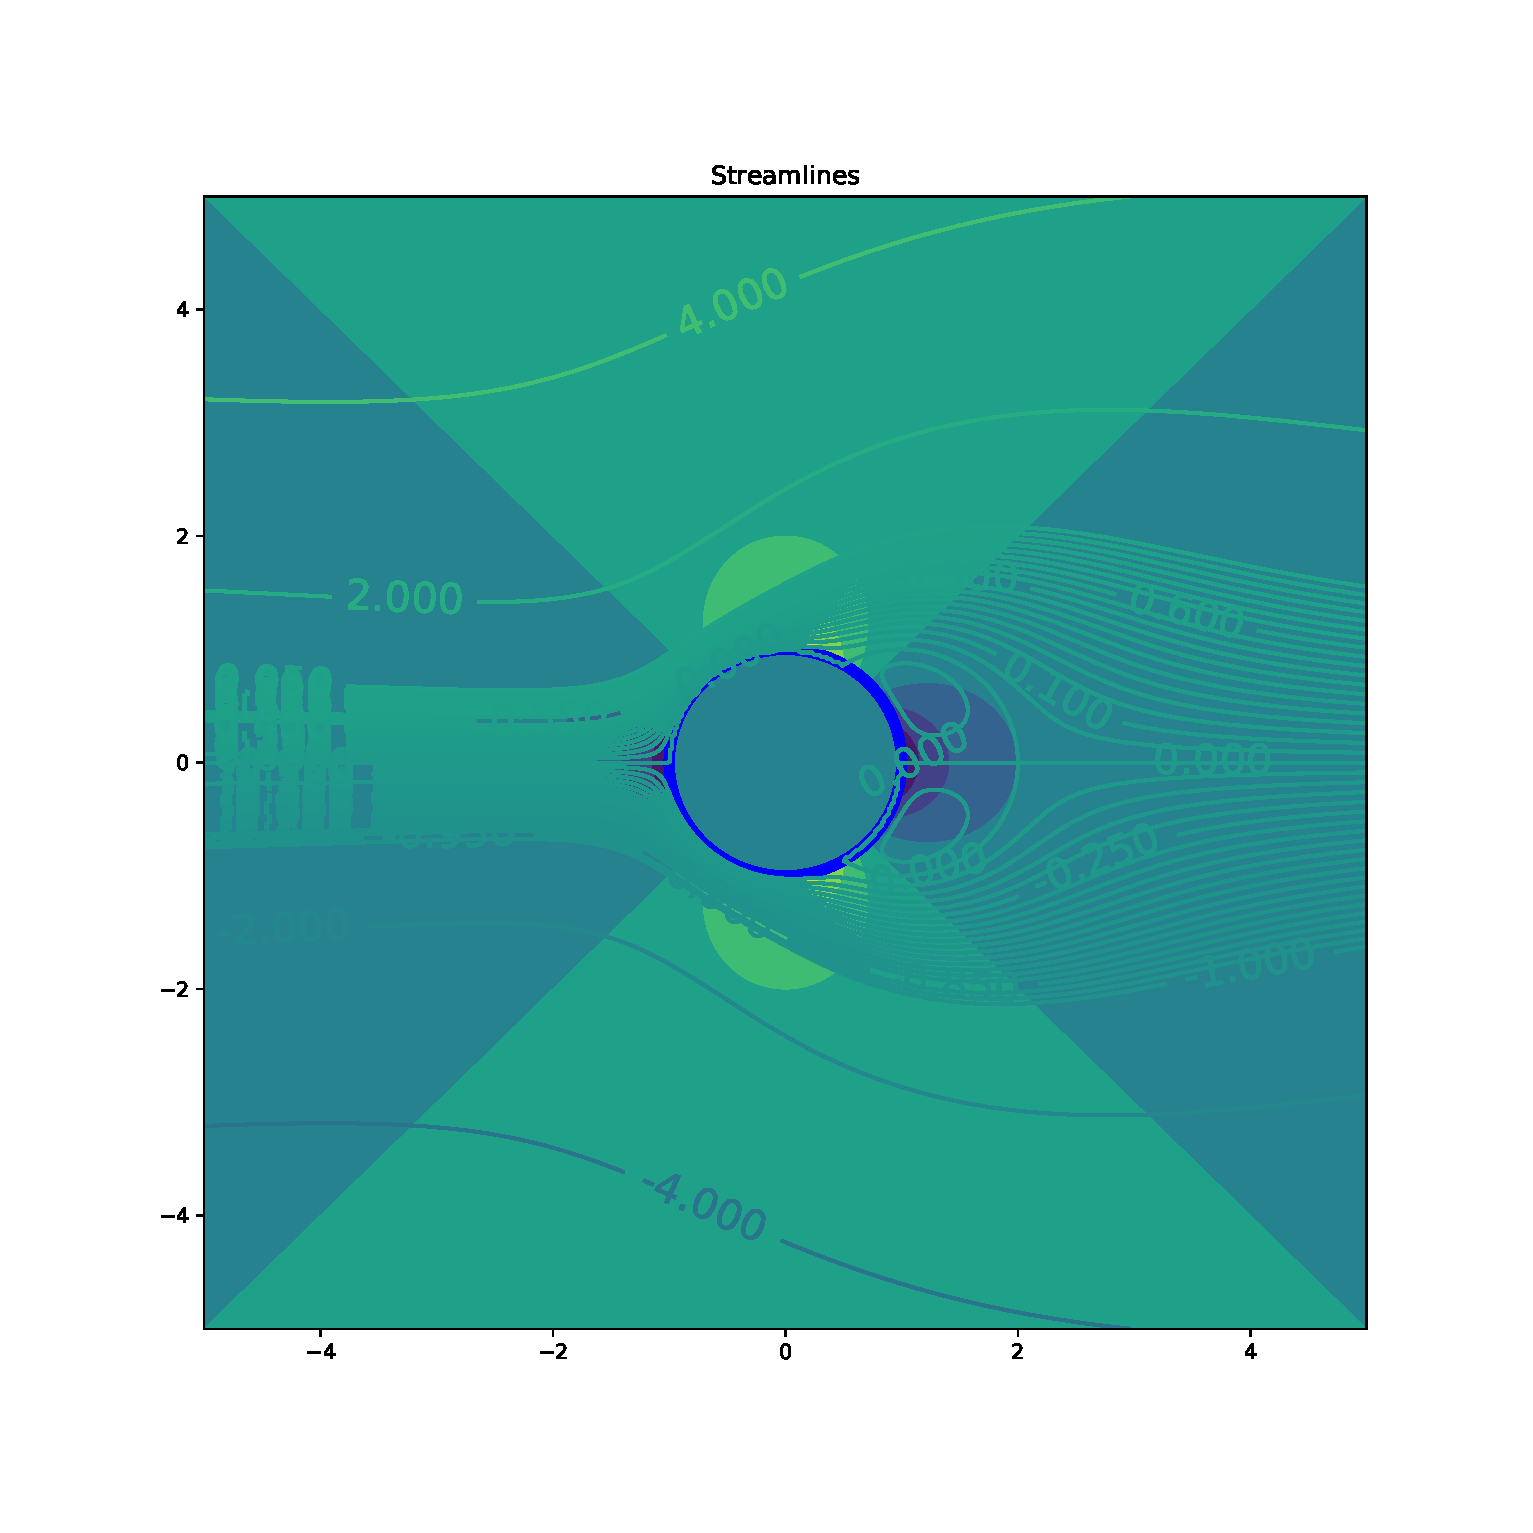
\includegraphics[width=0.8\linewidth]{figures/creeping_flow_past_cyl_slip}
  \caption{\label{fig:creeping_flow_past_cyl}}
\end{figure}


\begin{figure}
  \centering
  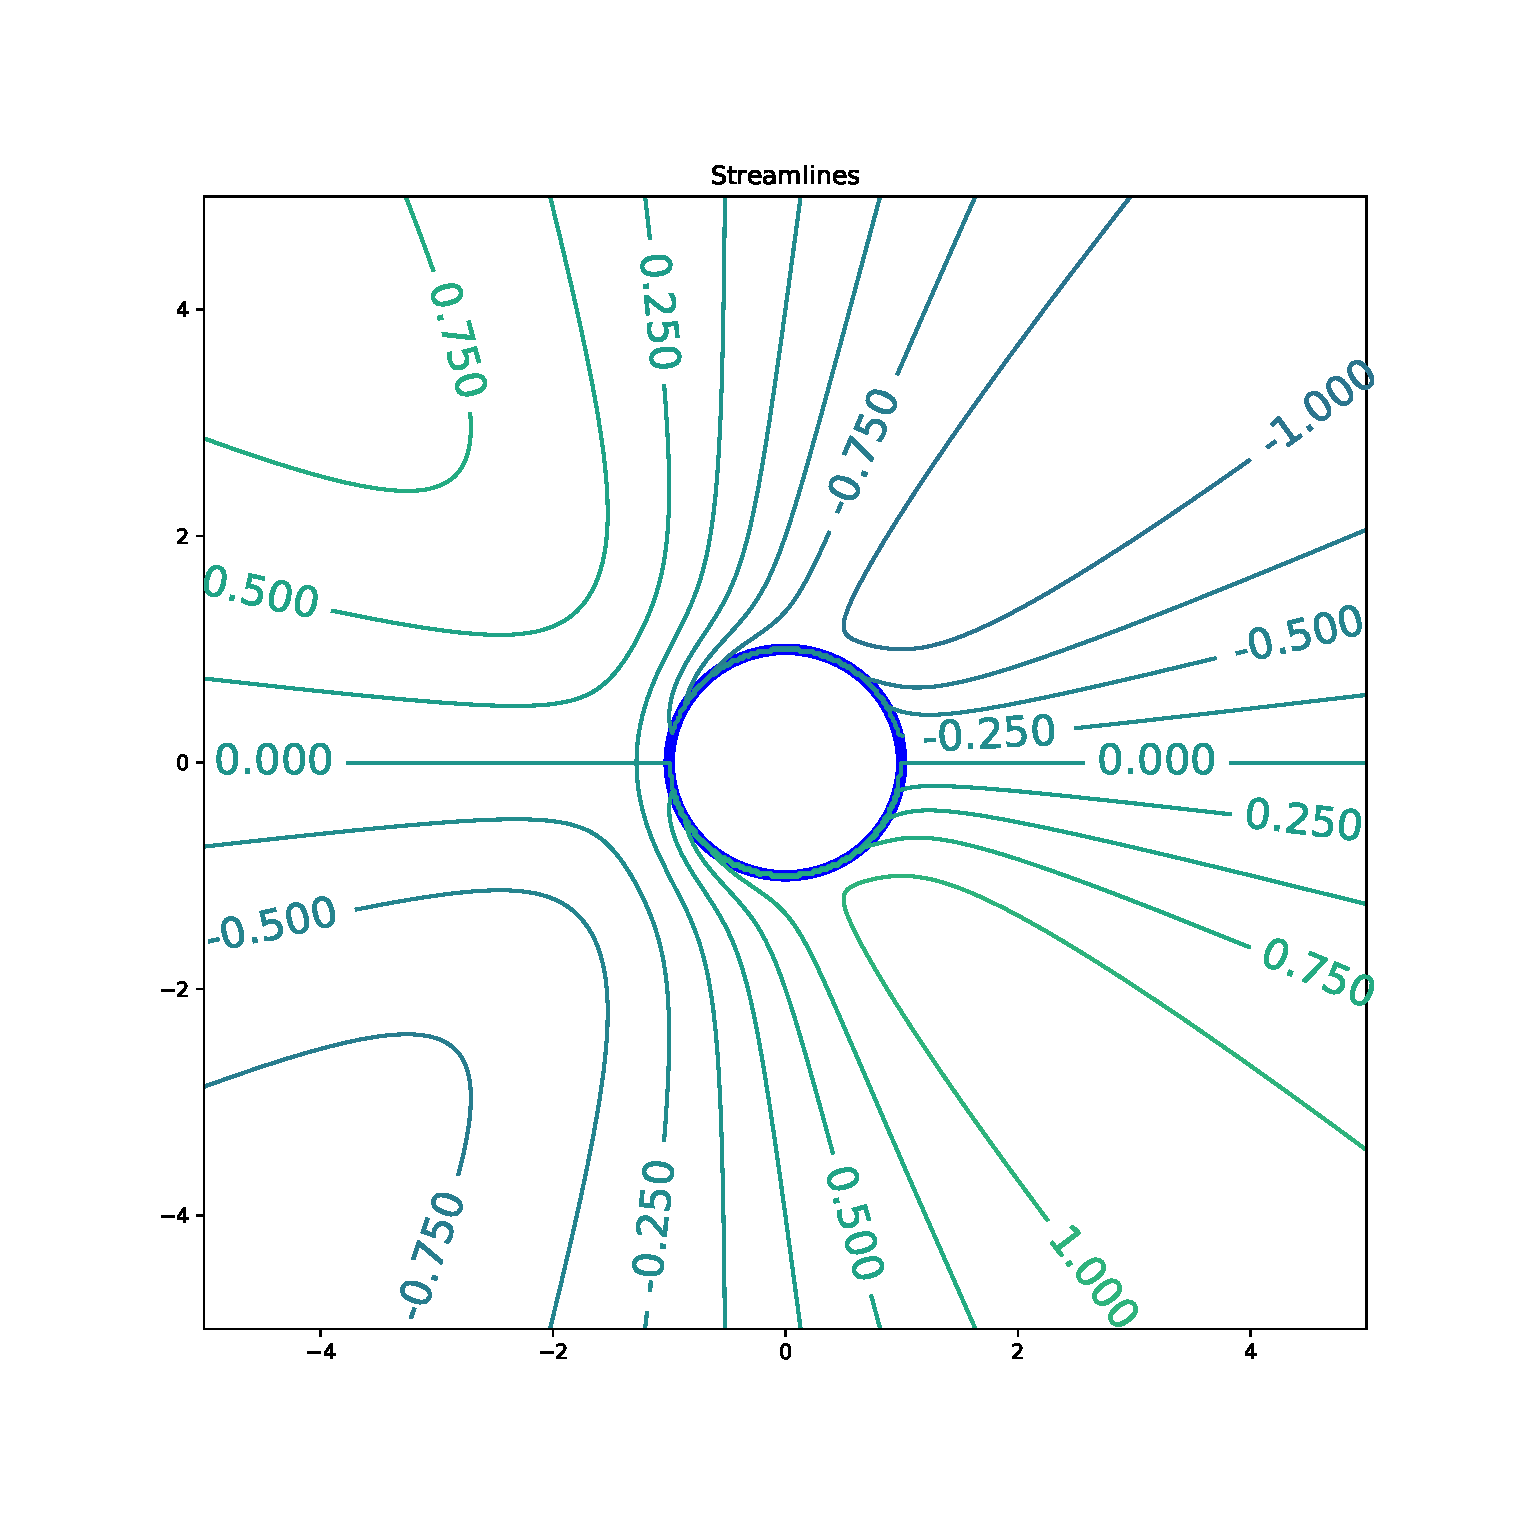
\includegraphics[width=0.8\linewidth]{figures/creeping_flow_past_cyl_slip_moving}
  \caption{\label{fig:creeping_flow_past_cyl_moving}}
\end{figure}


The resulting pressure field only has a non-trivial contribution from
the $\alpha=0$ term, since all other three are harmonic
(i.e. solutions of Laplace equation.)

The vector Laplacian is given by
\begin{align*}
(\nabla^2\bfu)_r &= \nabla^2 u_r - \frac{u_r}{r^2} - \frac{2}{r^2}
           \frac{\partial u_\theta}{\partial \theta} \\
(\nabla^2\bfu)_\theta &= \nabla^2 u_\theta - \frac{u_\theta}{r^2} + \frac{2}{r^2}
           \frac{\partial u_r}{\partial \theta} ,  
\end{align*}
with the scalar $\nabla^2$ expression as before in Eq.
\ref{eq:Lapl_in_polar}. We obtain
\begin{align*}
  (\nabla^2\bfu)_r &=   \frac{8 R u_0}{r^3} \cos(2 \theta)  \\
  (\nabla^2\bfu)_\theta &=    \frac{8 R u_0}{r^3} \sin(2 \theta)   .
\end{align*}

The pressure field is obtained from $\nabla p = \mu \nabla^2 \bfu$,
which in polar coordinates reads
\begin{align*}
  (\nabla p)_r     &=               \frac{\partial p }{  \partial r } = \mu(\nabla^2\bfu)_r  \\
  (\nabla p)_\theta &=  \frac{1}{r} \frac{\partial p }{  \partial \theta } = \mu(\nabla^2\bfu)_\theta ,
\end{align*}
whose solution is
\[
  p =
  -\frac{4 \mu u_0 R }{r^2} \cos(2\theta) =
  -\frac{4 \mu u_0}{R} \left( \frac{R }{r} \right)^2 \cos(2\theta) .
\]
In the last expression we make it clear that the pressure value is set
by $\mu u_0 / R$, and therefore the total pressure force upon the
cylinder is $D_p \sim p L R \sim \mu u_0 L$. The drag force would then
be independent of the radius, as predicted in
Eq. \ref{eq:drag_cyl_guess}. This is all consistent, if somewhat
surprising, but nevertheless moot: this pressure field, with its
$\cos(2\theta)$, has a d'Alembert's paradox! Indeed, by the same
arguments as in the classical potential solution, the net pressure
force is null. This is obvious in
Fig. \ref{fig:creeping_flow_past_cyl}, where the pressure field shows
a left-right symmetry.  Mathematically,
\begin{equation}
  \label{eq:pressure_drag_on_cyl_creeping}
  \frac{  D_p }{L} =
    R \int_0^{2\pi} d\theta   p \cos\theta  =
    4 \mu u_0 \int_0^{2\pi} d\theta  \cos\theta  \cos(2\theta)  = 0.
\end{equation}
Also, the sign of the pressure is troublesome: the low-pressure areas
are at the fore and aft of the cylinder, contrary to what may be
expected (and what is found for the potential solution,
Eq. \ref{eq:press_at_cyl_pot}.)

There is now another source of drag: shear stress on the surface. The
expression for the relevant part of the stress tensor is
\[
  \tau_{r\theta} = \mu \left(
    \frac1r
    \frac{\partial u_r}{\partial \theta} +
    r \frac{\partial }{\partial r} \left( \frac{u_\theta}{r}\right) 
  \right) 
\]
(i.e. it looks exactly as in spherical coordinates).

After some computations, at the surface we obtain
\[
  \tau_{r\theta} (R)  =  \frac{4 \mu u_0}{R} \left(
    \sin\theta - 2 \sin(2\theta) 
  \right) .
\]
The surprise is, then, that the term due to the potential solution,
$\sin\theta$, will result in a net drag force, but the new one will
not. Indeed, this force will be
\begin{equation}
  \label{eq:viscous_drag_on_cyl_creeping}
  \frac{  D_\tau }{L} =
   R \int_0^{2\pi} d\theta  (- \tau_{r\theta}) (- \sin\theta)  =
  4 \mu u_0 \int_0^{2\pi} d\theta  \sin^2\theta  =  4 \pi \mu u_0 .
\end{equation}
Notice there is a minus sign due to projection on the $x$ axis from
the tangential direction, and another due to the shear on the cylinder
being the reaction of the shear of the cylinder on the fluid.

The drag coefficient, defined as for the sphere (with an exposed area
now given by $2RL$), would be
\[
  C_\mathrm{inertial} = \frac{  2 D }{ \rho u_0^2 (2 R L) } =
  \frac{ 4 \pi \mu u_0   }{ \rho u_0^2  R L } =
  8\pi \frac{1}{\mathrm{Re}} ,
\]
with a Reynolds numberdefined in term of the diameter $2R$:
\[
  \mathrm{Re} = \frac{ \rho u_0 ( 2 R ) }{ \mu } .
\]

Notice that we have only employed two terms of what may be an
infinite expansion in terms $\sin(n\theta)$. In this way, by means of
Fourier analysis, we would be able to produce any tangencial velocity
we wished on the surface of the cylinder. The question is, of course,
which is the ``right'' distribution, since our main target, a null
velocity, is the one that is the one that is ruled out. For instance,
we could make the velocity null at the trailing edge of the cylinder
only.

Even if we did this, the potential would not be free of the
d'Alambert's paradox: all terms would ultimately be of the form
$\cos(n\theta)$, and the resulting drag would be zero for the same
reason as for $n=2$ in Eq. \ref{eq:pressure_drag_on_cyl_creeping}.

Moreover, the shear stress would also not change! Indeed, the new
terms in the stress tensor would be of the form $\sin(n\theta)$ ---
their contribution to the drag force would be null: in Eq.
\ref{eq:viscous_drag_on_cyl_creeping} it is clear that only $n=1$ may
contribute to this force. Since the only velocity contributing is the
potential solution, whose value is fixed by the up-stream velocity, it
cannot change.


\chapter{The viscous boundary layer}

\section{Stagnation flow}

In order to provide a glimse into the difficulties that are
encountered as soon as one ventures into slightly more complicated
problems, let us work out a solution of Navier-Stokes equations for a
simple stagnation situation.

The potential flow solution for a stady-state incompressible 2D
stagnation flow pattern close to a flat wall is given by the stream
function
\[
\psi = B x y ,
\]
from which,
\[
\begin{cases}
  & u_x =  \frac{\partial \psi}{\partial y} =   B x \\
  & u_y = -\frac{\partial \psi}{\partial x} = - B y .
\end{cases}
\]

The parameter $B$ has units of inverse time, and is given in practical
situations by $u_0 / L$, where $u_0$ is a relevant upstream velocity,
and $L$ a relevant size.

Recalling what we learned about potential flow and its relationship
with complex analysis, since $\psi = (B/2) \Im (z^2)$, it is easy to guess the
correct potential: $\phi=\Re( z^2) = (B/2) (x^2 + y^2)$.

This flow pattern looks roughly correct, see
Fig. \ref{fig:stagnation_streamlines} left, where the streamlines are
shown, along with the pressure. The latter follows from Bernoulli
principle:
\begin{equation}
  \label{eq:p_stag_pot}
p =
 -\frac{1}{2} \left[
  u_x ^2 +
  u_y^2
  \right] =
-\frac{1}{2} \left[
  (B x)^2 +
  (-B y)^2
  \right].  
\end{equation}


\begin{figure}
  \centering
  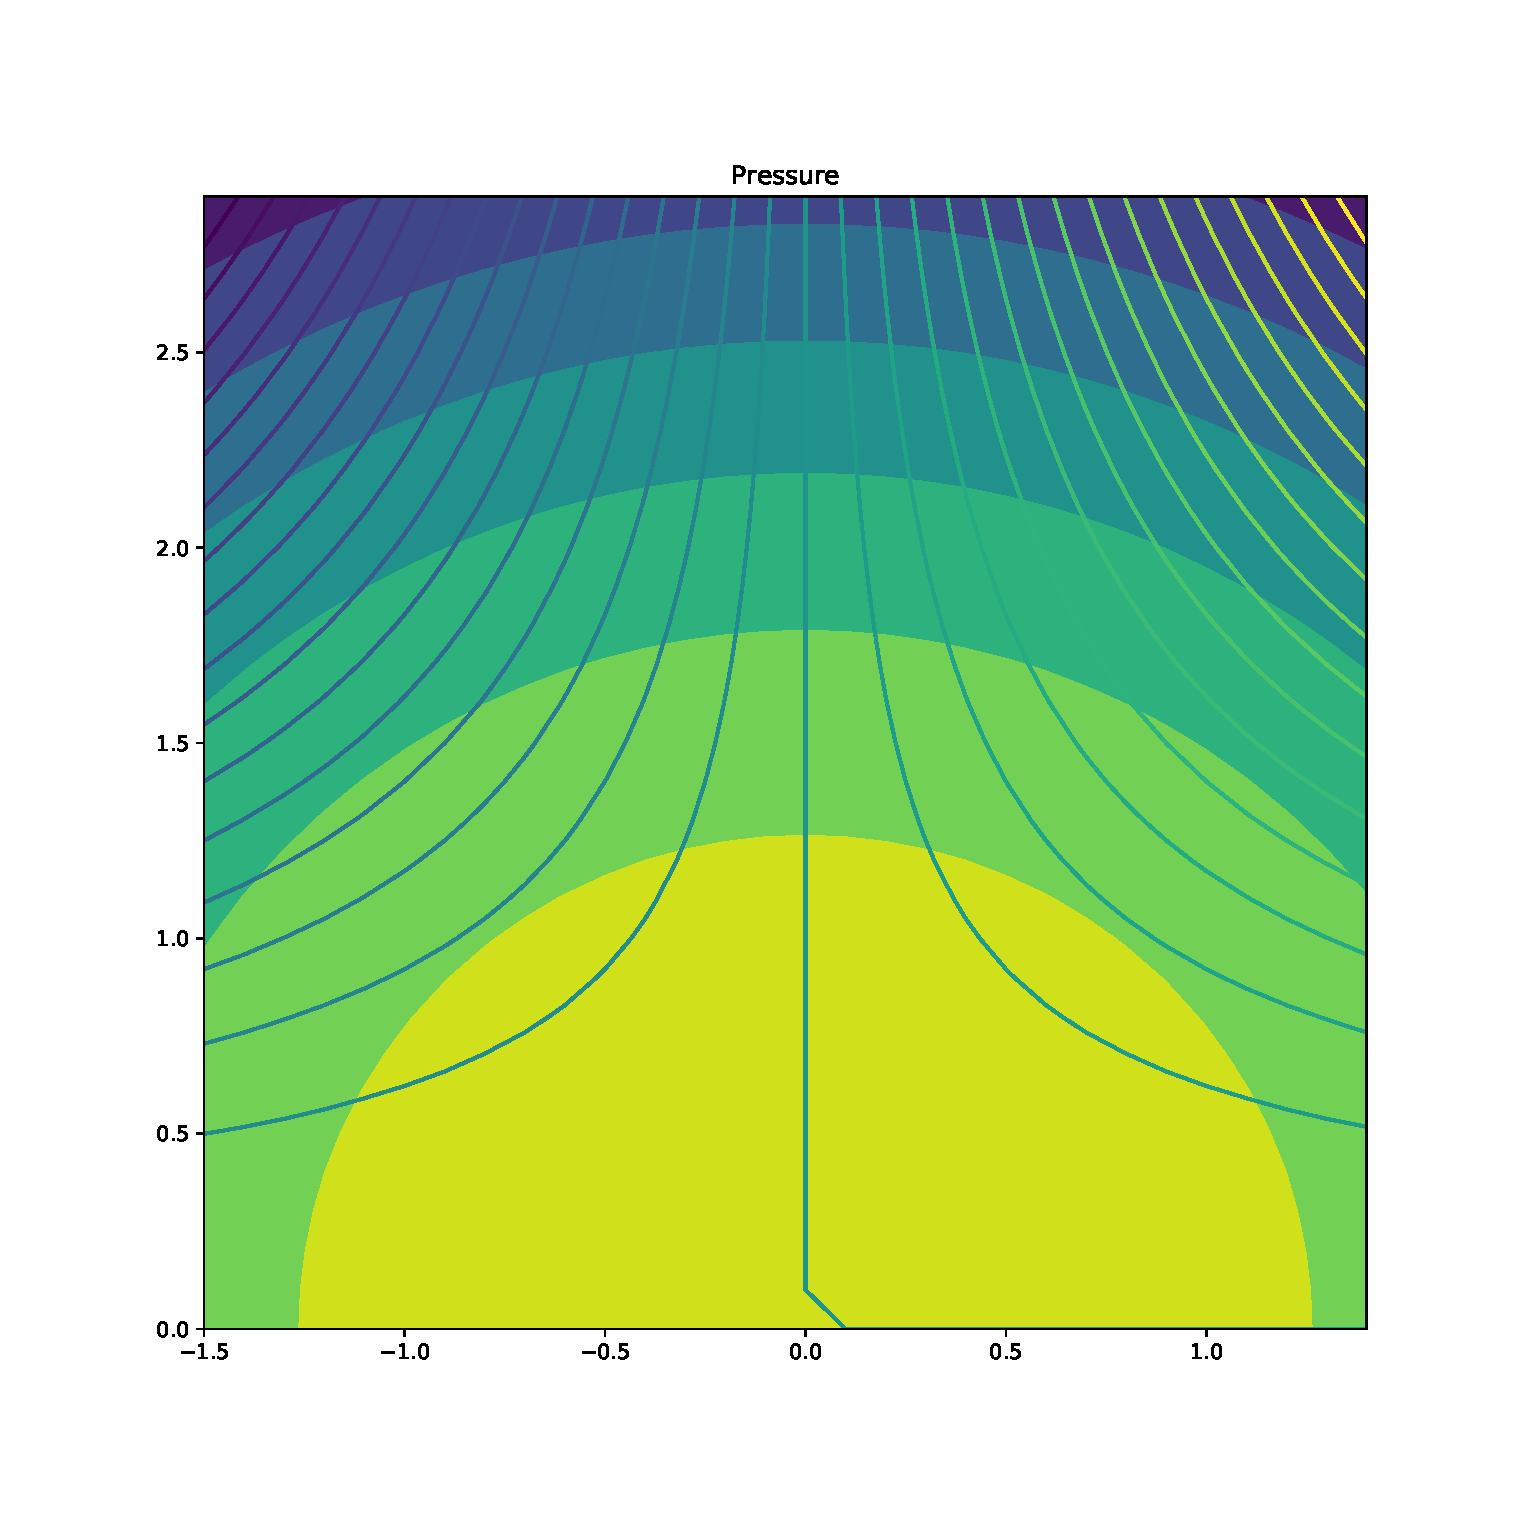
\includegraphics[width=0.4\linewidth]{figures/stagnation_potential_streamlines}
  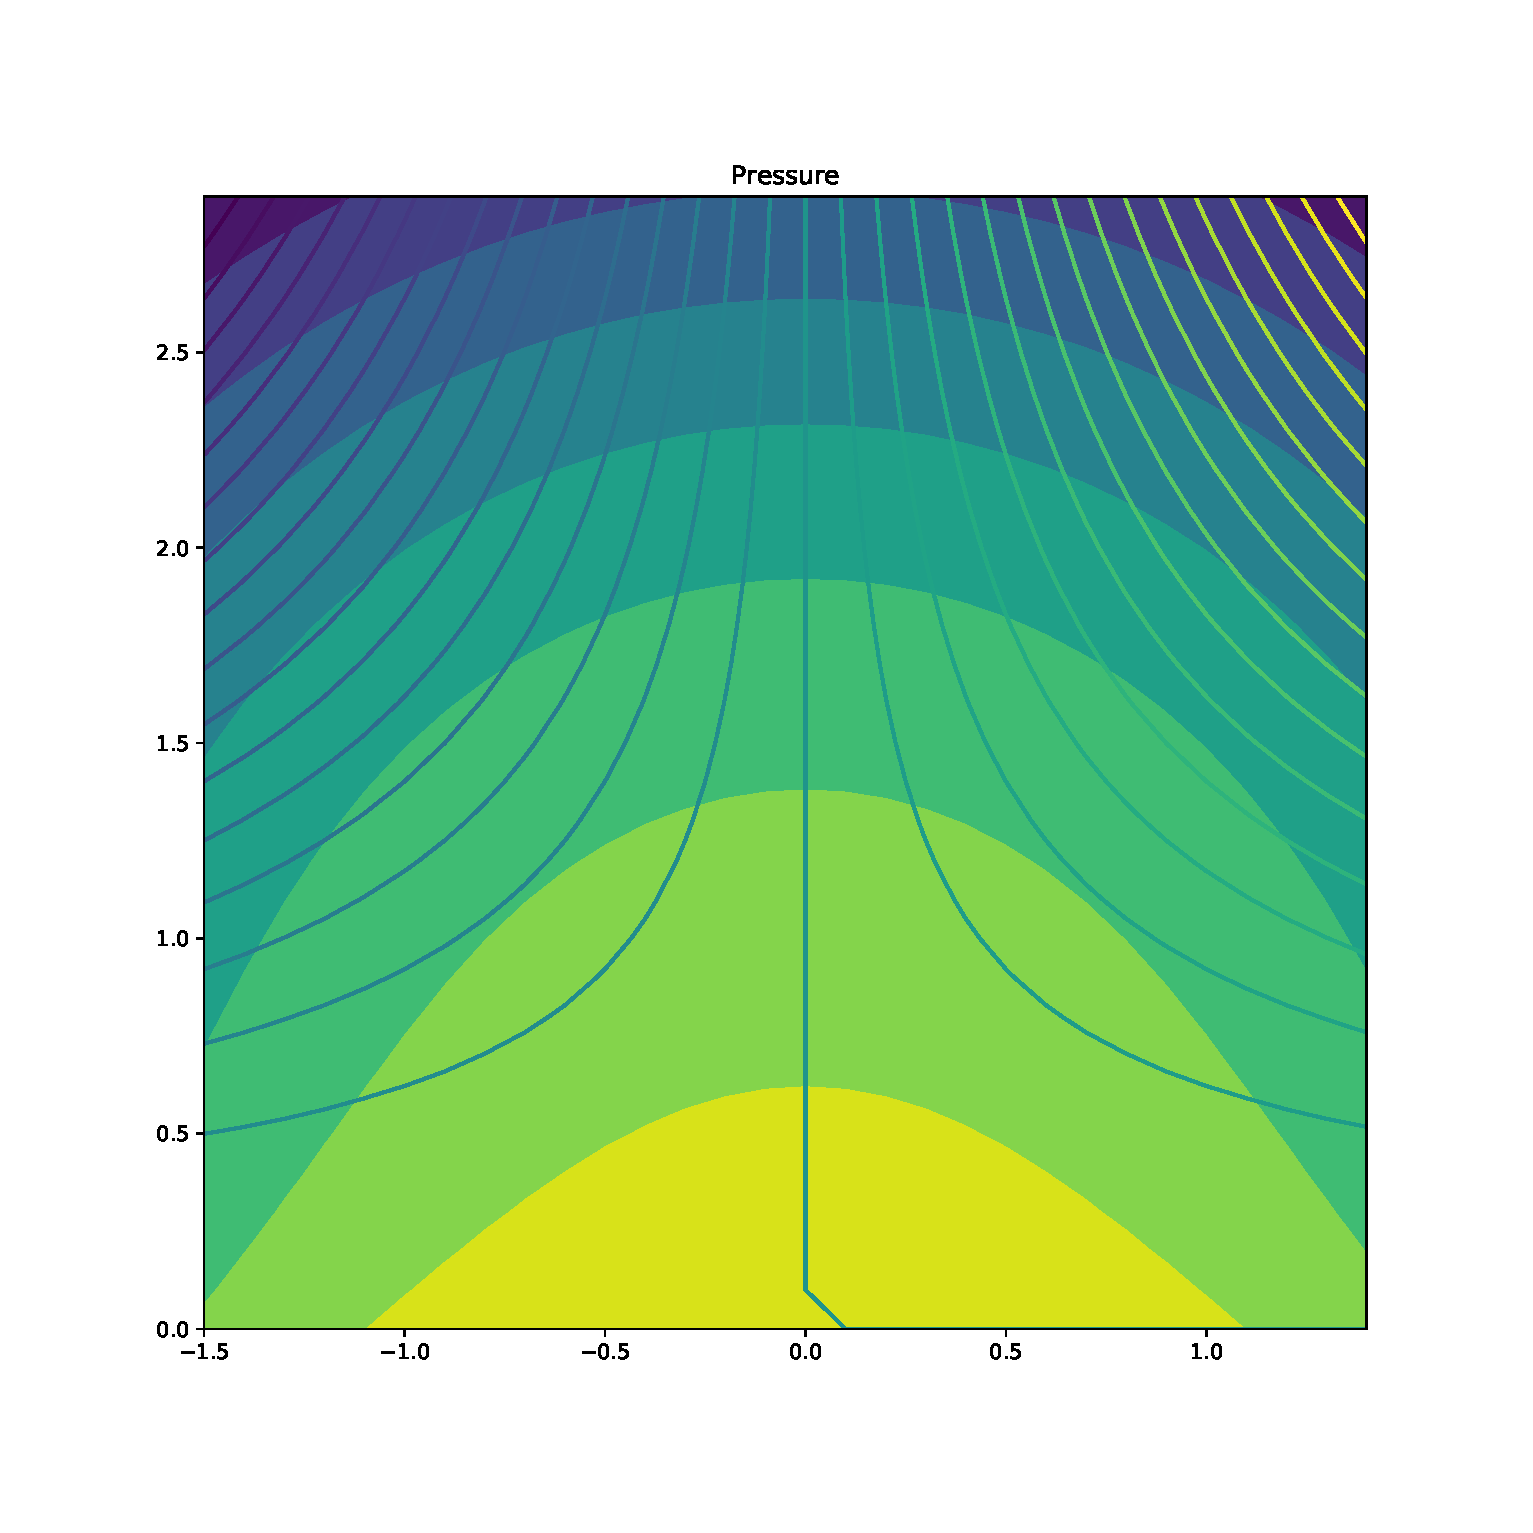
\includegraphics[width=0.4\linewidth]{figures/stagnation_viscous_streamlines}
  \caption{\label{fig:stagnation_streamlines}}
\end{figure}

But of course, at the wall ($y=0$) the fluid flows freely along the
wall. This means the boundary conditions are of the ``slip'' kind,
instead of the more realistic ``no-slip'' kind.

In order to find a correct flow, let us us the ansatz, originally
investigated by Hiemenz in 1911\footnote{%
  Hiemenz was a student of Prandtl, the founder of the theory of
  viscous boundary layers.
}.
  \[
\psi = B x f(y) ,
\]
where $f$ is a function of $y$ only. This is basically a separation of
variables, also guessing a linear dependence on $x$.

The velocity is now,
\[
\begin{cases}
  & u_x =   B x f' \\
  & u_y = - B f .
\end{cases}
\]
The correct no-slip condition then implies $f(0)=f'(0)=0$. We will
also require $f'(\infty)\to 1$ in order to recover our previous,
potential flow, solution.

Now, the steady 2D Navier-Stokes equations read
\begin{align}
  u_x  \frac{\partial u_x}{\partial x} +
  u_y  \frac{\partial u_x}{\partial y} 
  & =   - \frac{\partial p}{\partial x} +
  \nu
  \left(
  \frac{\partial^2 u_x}{\partial x^2} +
  \frac{\partial^2 u_x}{\partial y^2}
  \right) \\
  u_x  \frac{\partial u_y}{\partial x} +
  u_y  \frac{\partial u_y}{\partial y} 
  & =   - \frac{\partial p}{\partial y} +
  \nu
  \left(
  \frac{\partial^2 u_y}{\partial x^2} +
  \frac{\partial^2 u_y}{\partial y^2}
  \right) .
\end{align}
(Here, $p$ is not the true pressure, but the ``kinematic pressure'',
$p/\rho$. For convenience, a $\rho$ factor is assimilated into it, in
the same way that $\nu=\mu/\rho$.)

The $x$ equation is then reduced to
\[
 (B x f') (B f') + (-B f) B x f'' =  - \frac{\partial p}{\partial x} +
\nu B x f''' ,
\]
which may be written as
\[
B f f'' - B (f')^2 + \nu f''' = \frac{1}{B x} \frac{\partial
  p}{\partial x}  .
\]
Now, the left part of the equation is a function of $y$ only. This
means the pressure can only have this form:
\[
p(x,y) = C x^2 + h(y) ,
\]
with a constant $C$ and a function of $h$ to be determined later. Moreover,
as $y$ gets large we want to recover the potential solution. In this limit,
\[
f \to a + y \qquad f' \to 1 \qquad f'' \to 0 \qquad f'''\to 0 ,
\]
so the equation in this limit is
\[
- B \to  \frac{2 C x }{B x} ,
\]
which means $C =-B/2$, to be used later when solving for the pressure.

We must then solve
\[
 B \left(  f f'' + 1-  (f')^2 \right) + \nu f''' = 0 .
\]

Now, a lot may be learned from the shape of an equation without even
solving it. Let us look for a similarity transformation of the
form
\[
f(y) = b g(a y) ,
\]
so that equation for $f$ may be cast as an equation for $g$ with no
parameters. With this prescription,
\[
f' = ba g' \qquad f''=b a^2 g'' \qquad f'''= b a^3 g''' ,
\]
So then the equation reads
\[
 B \left(  b^2 a^2 g g'' + 1-  b^2 a^2 (g')^2 \right) + \nu b a^3  g''' = 0 .
\]
Because of the ``$1$'' in the parenthesis, it is clear $b=1/a$, so then,
\[
 B \left(  g g'' + 1-  (g')^2 \right) + \nu  a^2  g''' = 0 .
\]
Therefore, if $a=\sqrt{B/\nu}$,
\begin{equation}
  \label{eq:Z_ode}
  g g'' + 1-  (g')^2  +  g''' = 0 ,
\end{equation}
with no parameters, as we wanted. This means that, whichever solution
we find, our $f$ is going to be given by
\[
f(y) = \sqrt{\frac{\nu}{B}} g\left(\sqrt{\frac{B}{\nu}}  y  \right) =
\sqrt{\frac{\nu}{B}} g\left(\frac{y}{ \sqrt{\nu/B} } \right) =
 \ell g\left(\frac{y}{ \ell } \right) .
\]
Clearly, $\ell = \sqrt{\nu/B} $ sets the scale of variation of the
flow away from its potential solution.

Notice that the velocities will be
\[
\begin{cases}
  & u_x =   B x g'(y/\ell) = B\ell \frac{x}{\ell} g'(y/\ell)  \\
  & u_y = - B \ell g(y/\ell)  ,
\end{cases}
\]
so that the velocity scale is set by $B\ell=\sqrt{B\nu}$.


%The $y$ equation reduces, with our velocities, to
%\[
%B^2 f f' = - \frac{\partial p}{\partial y} - B\nu f'' .
%\]
%This means that $\frac{\partial p}{\partial y}$ is a function of $y$
%only.



Our task is then to integrate the non-linear ODE \ref{eq:Z_ode}, subject
to these boundary conditions:
\[
g(0)=0 \qquad g'(0)=0 \qquad g''(x\to \infty) \to 0 .
\]
If we had a condition on $g''(0)$, the problem would be a
straight-forward exercise in integration. However, we have instead a
condition on the other side of the integration domain, which makes
this problem somewhat harder. The technique should then be a
``shooting method'', in which $g''(0)$ is adjusted until a vanishing
small of $g''$ far away is found. The procedure may be made
systematic, but we can also fiddle a bit with the parameters in order
to find a reasoable approach. It is quite easy to arrive at
$g''(0)\approx 1.234$, as in the jupyter python notebook at
Supplementary Material.

%How far is far away may be again estimated from the equation.


\begin{figure}
  \centering
  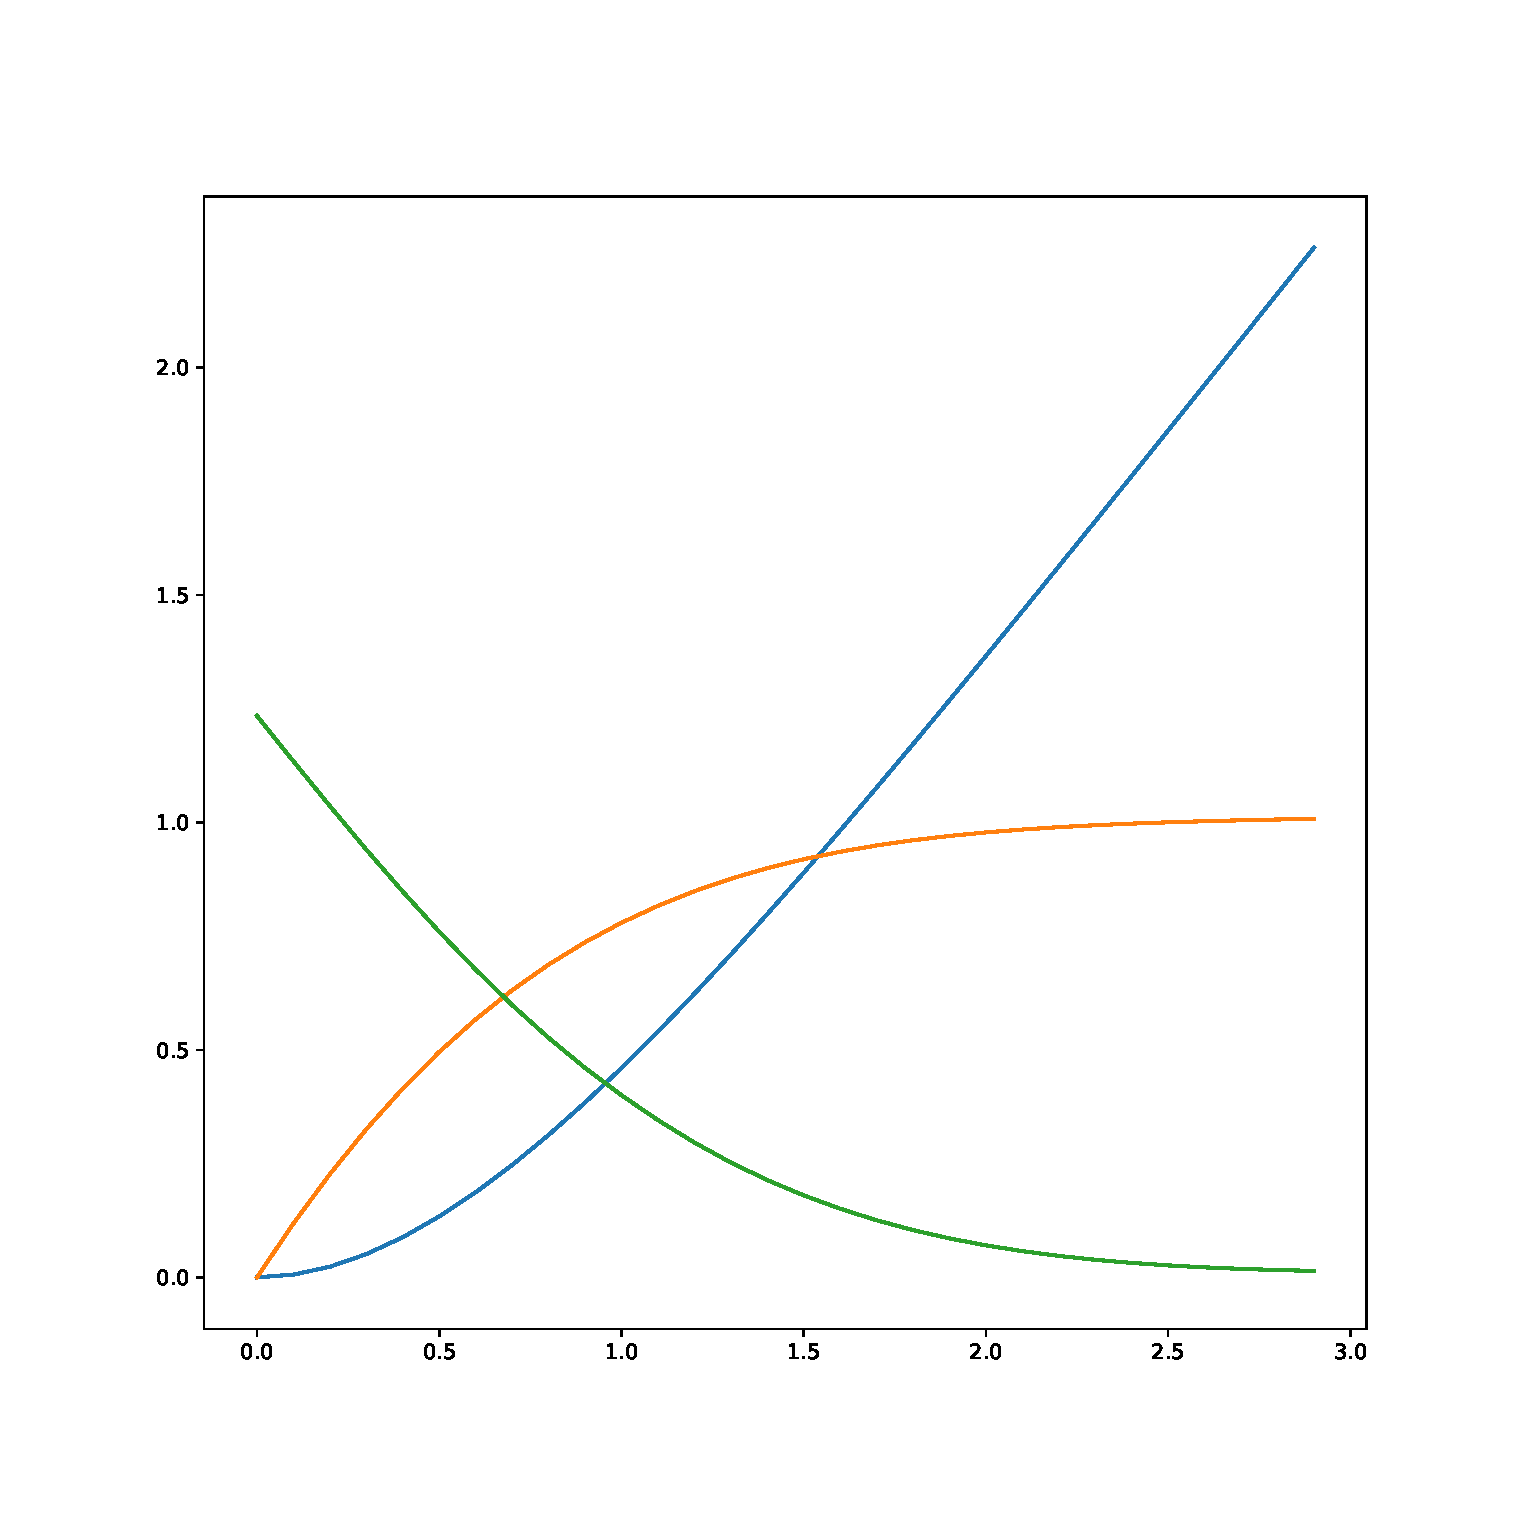
\includegraphics[width=0.4\linewidth]{figures/stagnation_functions}
    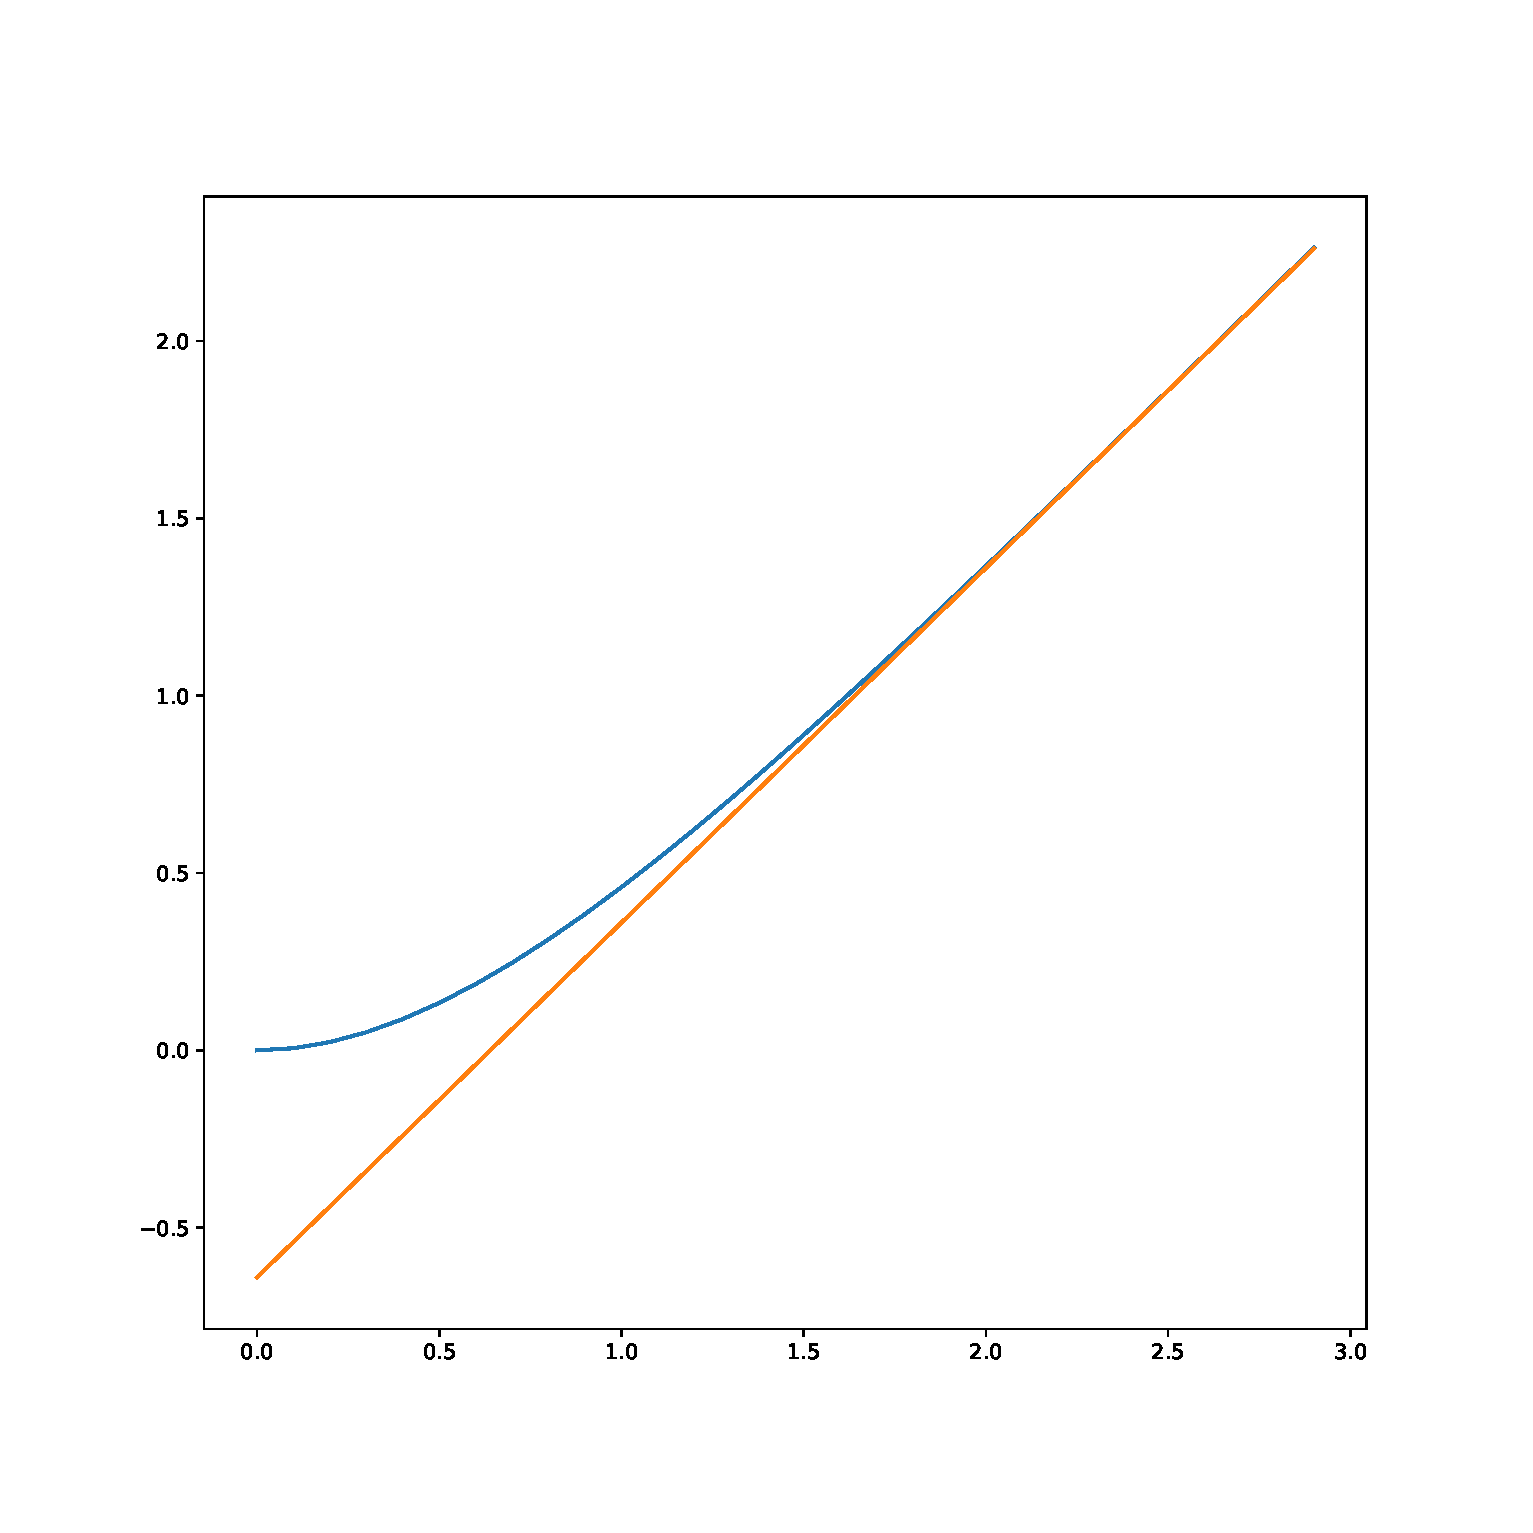
\includegraphics[width=0.4\linewidth]{figures/stagnation_function_disp}
  \caption{\label{fig:stagnation_functions}}
\end{figure}


In Figure \ref{fig:stagnation_functions} left, the function $g$ and
its first and second derivatives are plotted. With these, it is easy
to plot the resulting streamlines, Figure
\ref{fig:stagnation_streamlines} right. In the latter, the potential
streamlines are shown in the left. It is apparent how the flow is
``moved upwards'' due to viscous effects near the wall. This
displacement is readily quanfified by the asympotic behavour of $g$,
as shown in Figure \ref{fig:stagnation_functions} left. A reasonable
approximation is
\[
g(y) \approx -0.64 + y .
\]
This provides an estimate of the boundary layer thickness as given
by
\[
\delta = 0.64 \ell =  0.64 \sqrt{\nu/B} ,
\]
which then increases as the root square of $\nu$, and decreases as,
basically, the root square of the velocity far away from the wall
(through $B$).

To get some numbers, if air approaches a \SI{10}{\centi\meter}
diameter cylinder at $u_0=\SI{10}{\meter\per\second}$, then
$B = 4u_0/D =\SI{400}{\per\second}$ (there is a factor of $4$
involved, see \cite{white1991viscous} \S 7.3 ). With
$\nu\approx\SI{1.5e-5}{\meter\squared\per\second}$, we get
$\delta = \SI{0.12}{\milli\meter}$, a very thin layer. The thickness
of the layer can be defined in other ways, for example as the distance
at which $f'(y) \approx 0.99 $ (so that the value of $u_x = B x f'$ is
$99\%$ its potential solution value, $B x$.) This yields
$\approx 2.4 \ell$, which is about $3.7$ times larger than
$\delta$. Still, only approximately $ \SI{0.44}{\milli\meter}$, beyond
which the effect of the wall is quite neglibible.

This fact is a blessing, since it restores our faith in
potential-based solutions: many flows look potential flows when viewed
at some distance from obstacles (indeed, away from any region that may
generate vorticity and involve shear, such as jets, wakes \ldots). It
also solves d'Alembert's paradox, since the velocity field can still
comply with the no-slip boundary condition and exert drag forces on
obstacles (in general, they will be due both to pressure and to wall
shear stress). It is also a curse mathematically: the details of a
proper matching between it the layer and the flow around it must be
worked out carefully. Also computationally, the fact that the boundary
layer is so thin compared with other dimensions of the problem leads
to prohibitively large simulation meshes, or the necessity to refine
the meshes close to surfaces. The latter fact favours methods such as
the finite element method, or the finite volume method, in which
refinement is easier, over other ones like finite differences.

The pressure was partly known already, $p=-(B^2/2) x^2 + h(y)$. The other
Navier-Stokes equation, which we have still not used, reads
\[
B f B f'  =  - \frac{\partial p}{\partial y} -
\nu B  f'' .
\]
This means
\[
h' = - B^2 f f' - \nu B f'' ,
\]
which may be easily integrated :
\[
h = -B^2 \frac12 f^2  - \nu B f' .
\]
So, finally:
\[
p = -\frac{1}{2} \left[
  (B x)^2 +
  (B f)^2
  \right]  - \nu B f' =
 -\frac{1}{2} \left[
  (u_x / f' )^2 +
  u_y^2
  \right]  - \nu B f' ,
 \]
 where the last equality shows that the pressure is not so different
 from the potential solution, Eq. \ref{eq:p_stag_pot}.
%
 Notice it is not $u_X$ which features, but rather $u_x/f'$, which
 does tend to the $u_x$ away from the wall. An additional, viscous
 term appears, which makes the pressure have a constant offset
 $-\nu B$ with respect to its potential counterpart, as we move
 away from the wall.

 Pressures are also included in Fig.
 \ref{fig:stagnation_streamlines}. To make a more quantitative
 comparison, isobars are plotted in
 Fig. \ref{fig:stagnation_pressures}. It is interesting that viscosity
 causes pressure to be ``pushed'' against the wall, flattening the
 isobars (and, interestingly, making them not normal to the
 wall). While, far away from the wall, they approach the same circular
 shape, but with a constant offset. In these figures, pressures are
 plotted in their reduced form. It is easy to check that the pressure
 scale is given by $B \nu$ (units of velocity squared --- remember this
 is the dynamic pressure).

\begin{figure}
  \centering
  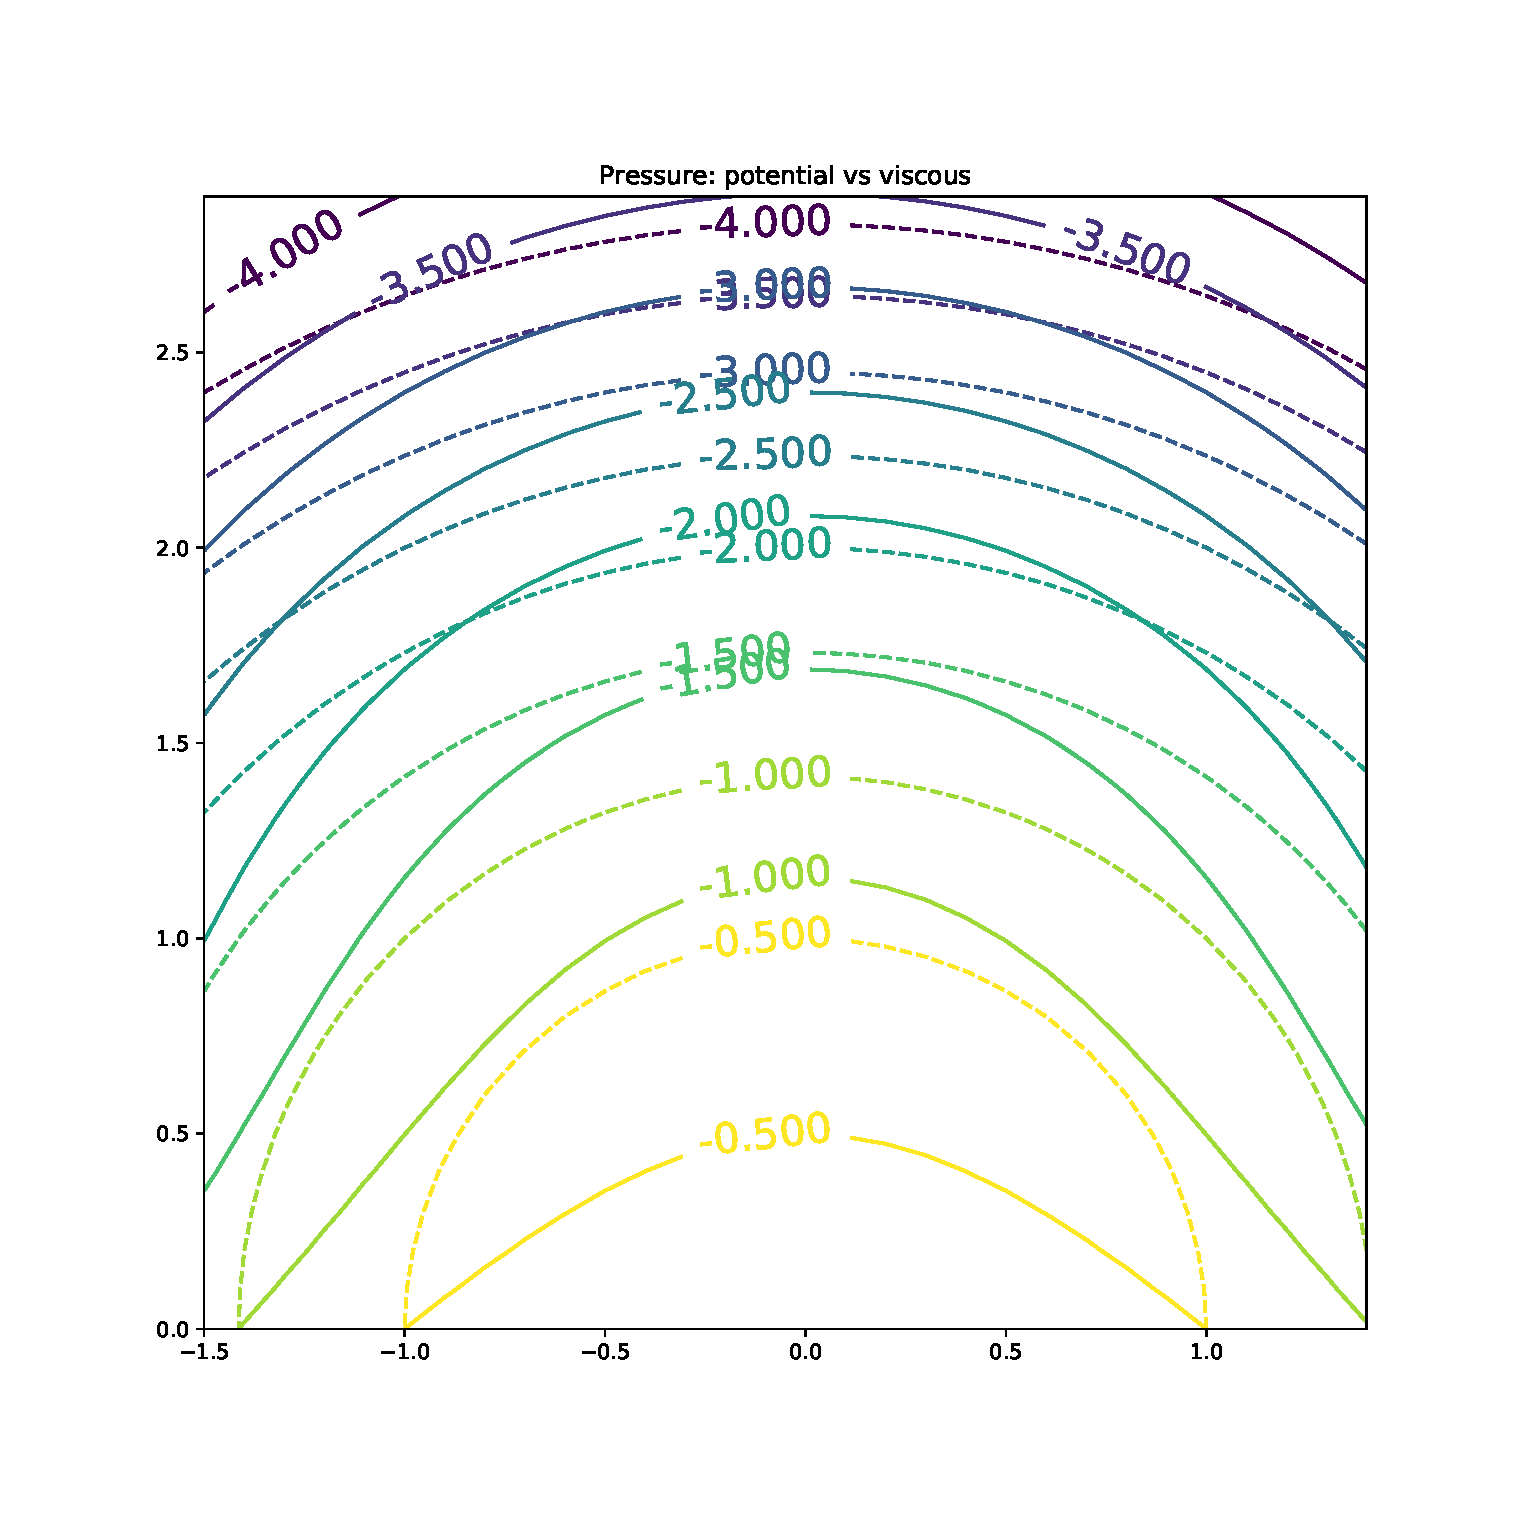
\includegraphics[width=0.6\linewidth]{figures/stagnation_potential_viscous_pressures}
  \caption{\label{fig:stagnation_pressures}}
\end{figure}

Another interesting feature of the flow is its vorticity, which is
readily computed from
\[
\omega_z =
\frac{\partial u_y}{\partial x} -
\frac{\partial u_x}{\partial y} =
0 - B x f''(y)  = - B x^* g''(y^*) .
\]
Hence the wall is seen to induce vorticity close to it, with a sign change
on both sides on the $x=0$ symmetry plane. The shear stress is given by a
similar expression,
\[
\tau_{xy}= \mu
\left(
\frac{\partial u_y}{\partial x} +
\frac{\partial u_x}{\partial y}
\right)
 =  \mu B  x f''(y)  = \mu B x^* g''(y^*) .
 \]

 In particular, the wall stress is
 \[
 \tau_\mathrm{w}:=\tau_{xy}(y=0) = \mu B x^* g''(0)
 \approx 1.234 \mu B x^*
 \]

 The (horizontal) skin friction coefficient may be defined, for this problem,
 as
 \[
 C_\mathrm{f} := \frac{2 \tau_\mathrm{w} }{ \rho (B x)^2 } .
 \]
 The denominator features the horizontal velocity away from the wall,
 $B x$. Then,
 \[
 C_\mathrm{f} := \frac{2 \sqrt{B\nu}  g''(0) }{ B x } =:
 \frac{2   g''(0) }{\sqrt{ \mathrm{Re}_x} } ,
 \]
 where the local Reynolds number is defined as
 \[
 \mathrm{Re}_x = \frac{(Bx) x}{\nu} .
 \]
 I.e. a Reynolds number where the typical velocity is the horizontal
 velocity far from the wall, $Bx$, and the distance is that to the
 impact point, $x$. A dependence of the friction coefficient with the
 inverse square root of a local Reynolds number is a common feature of
 laminar boundary layers.
 


%\chapter{Turbulence}

%\input{etc}

\printindex

\begin{appendix}
   \listoffigures
   \listoftables
\end{appendix}



\end{document}
